The following section aims to investigate the performance of techno-economically optimised single flash \ac{DSC} and binary \ac{ORC} geothermal power plants for two-phase geothermal heat sources.

\subsection{Plant Configurations}
    The power plant configurations used for the techno-economic optimisation are the same as those used for the thermodynamic optimisation, see Section~\ref{sec:prosim_plant_configurations}.

\subsection{Boundary Conditions}
    The boundary conditions used for the techno-economic optimisation are the same as those used for the thermodynamic optimisation, see Section~\ref{sec:prosim_thermo_BCs}.

\subsection{Optimisation Configuration}
    The performance of the power plants is optimised based on the specific plant cost, by adjusting the process variables. For the \ac{DSC} plant, the flash pressure and the condensation pressure, as well as the minimum temperature in the condenser are adjusted; for the binary \ac{ORC} plant, the evaporation pressure, the degree of super-heating and the condensation temperature, as well as the minimum approach temperature differences in the pre-heater, evaporator, super-heater and condenser are adjusted,  Table~\ref{table:prosim_pure_water_techno_opt_params}, .

    \begin{table}[H]
        \centering
        \caption{The optimisation parameters used for the single flash \ac{DSC} and the binary \ac{ORC} geothermal power plants.}
        \label{table:prosim_pure_water_techno_opt_params}
        \begin{tabular}{|c | c c |}
    \hline
    \rowcolor{bluepoli!40} % comment this line to remove the color
      & \textbf{Single Flash DSC} & \textbf{Binary ORC} \T\B \\
    \hline \hline
    Objective Function & \(c_{plant}\) & \(c_{plant}\) \T\B \\
    \hline
    \multicolumn{1}{|l|}{\multirow{7}{*}{Controls}} & \qty{0.1}{\bar}\(\leq P_{cond}\leq\)\qty{5.0}{\bar} & \qty{303}{\K}\(\leq T_{cond}\leq\)\qty{400}{\K} \T\B \\
    \multicolumn{1}{|l|}{} & \num{0.3}\(\leq \frac{P_{flash]}}{P_{in}}\leq\)\num{1.0} & \num{0.2}\(\leq \frac{P_{evap}}{P_{crit}}\leq\)\num{0.8} \T\B \\
    \multicolumn{1}{|l|}{} & \qty{2}{\K}\(\leq \Delta T_{cond}^{min}\leq\)\qty{30}{\K} & \qty{3}{\K}\(\leq \Delta T_{sh}\leq\)\qty{15}{\K} \T\B \\
    \multicolumn{1}{|l|}{} &  & \qty{2}{\K}\(\leq \Delta T_{preh}^{min}\leq\)\qty{30}{\K} \T\B \\
    \multicolumn{1}{|l|}{} &  & \qty{2}{\K}\(\leq \Delta T_{evap}^{min}\leq\)\qty{30}{\K} \T\B \\
    \multicolumn{1}{|l|}{} &  & \qty{2}{\K}\(\leq \Delta T_{suph}^{min}\leq\)\qty{30}{\K} \T\B \\
    \multicolumn{1}{|l|}{} &  & \qty{2}{\K}\(\leq \Delta T_{cond}^{min}\leq\)\qty{30}{\K} \T\B \\
    \hline
\end{tabular}        
    \end{table}

\subsection{Performance Analysis: DSC}

    The techno-economic optimisation of the \ac{DSC} geothermal power plant reduces the specific plant costs by between \qty{7}{\percent} and \qty{10}{\percent},  Figure~\ref{fig:prosim_purewater_DeltaSpecCost_DSC_thermo_vs_techno}, at the expense of between \qty{10}{\percent} to \qty{35}{\percent} of net plant power, Figure~\ref{fig:prosim_purewater_DeltaWnet_DSC_thermo_vs_techno}.

    \begin{figure}[H]
        \centering
        \resizebox{\linewidth}{!}{% This file was created with tikzplotlib v0.10.1.
\begin{tikzpicture}

\definecolor{chocolate2369815}{RGB}{236,98,15}
\definecolor{crimson2143940}{RGB}{214,39,40}
\definecolor{darkgray165}{RGB}{165,165,165}
\definecolor{darkgray176}{RGB}{176,176,176}
\definecolor{darkgreen06827}{RGB}{0,68,27}
\definecolor{darkorange25512714}{RGB}{255,127,14}
\definecolor{darkseagreen133204132}{RGB}{133,204,132}
\definecolor{darkslategray45}{RGB}{45,45,45}
\definecolor{dimgray108}{RGB}{108,108,108}
\definecolor{firebrick175572}{RGB}{175,57,2}
\definecolor{forestgreen4416044}{RGB}{44,160,44}
\definecolor{forestgreen611448}{RGB}{6,114,48}
\definecolor{gainsboro216}{RGB}{216,216,216}
\definecolor{lightgray198232191}{RGB}{198,232,191}
\definecolor{lightgray204}{RGB}{204,204,204}
\definecolor{lightgreen160216154}{RGB}{160,216,154}
\definecolor{mediumpurple148103189}{RGB}{148,103,189}
\definecolor{navajowhite253207161}{RGB}{253,207,161}
\definecolor{saddlebrown127394}{RGB}{127,39,4}
\definecolor{sandybrown25315378}{RGB}{253,153,78}
\definecolor{sandybrown253173106}{RGB}{253,173,106}
\definecolor{seagreen5816488}{RGB}{58,164,88}
\definecolor{sienna1408675}{RGB}{140,86,75}
\definecolor{silver188}{RGB}{188,188,188}
\definecolor{steelblue31119180}{RGB}{31,119,180}

\begin{groupplot}[
    group style={
        group size=2 by 3, 
        vertical sep=2.5cm, 
        horizontal sep=2.5cm},
    height=6cm, 
    width=7cm, 
]
\nextgroupplot[
legend cell align={left},
legend style={
  fill opacity=0.8,
  draw opacity=1,
  text opacity=1,
  at={(1.15,-0.35)},
  anchor=north,
  draw=lightgray204
},
legend columns=3,
tick align=outside,
tick pos=left,
x grid style={darkgray176},
xlabel={Inlet Steam Quality/\unit{\percent}},
xmin=-5, xmax=105,
xtick style={color=black},
y grid style={darkgray176},
ylabel={Specific Cost/\unit{\USD\of{2023}\per\kilo\watt}},
ymin=0, ymax=5133.20005020261,
ytick style={color=black},
ytick distance=1000
]
\addplot [semithick, gainsboro216]
table {%
0 -1
1 -1
};
\addlegendentry{\(T_{geo}^{in}=\)\qty{423}{\K}}
\addplot [semithick, navajowhite253207161, forget plot]
table {%
0 4888.7143335263
10 3404.0250225565
20 2765.54563623294
30 2409.1559187536
40 2183.27858115757
50 2009.69985620321
60 1878.59416928319
70 1781.0224664262
80 1687.7740515826
90 1617.80913453152
100 1554.39592832416
};
\addplot [semithick, silver188]
table {%
0 -1
1 -1
};
\addlegendentry{\(T_{geo}^{in}=\)\qty{448}{\K}}
\addplot [semithick, sandybrown253173106, forget plot]
table {%
0 4151.52655916405
10 3093.66458210808
20 2505.74674359629
30 2179.5159627031
40 1957.18513763749
50 1799.12235928086
60 1671.81829312684
70 1573.71545917379
80 1494.37146800752
90 1427.06656072871
100 1352.99672129195
};
\addplot [semithick, darkgray165]
table {%
0 -1
1 -1
};
\addlegendentry{\(T_{geo}^{in}=\)\qty{473}{\K}}
\addplot [semithick, sandybrown25315378, forget plot]
table {%
0 3655.98032140456
10 2848.07438984096
20 2334.75521170762
30 2013.49500986261
40 1811.64639061245
50 1658.35478306289
60 1536.22860528175
70 1435.11969747933
80 1358.52998816526
90 1292.05743230332
100 1238.4966377997
};
\addplot [semithick, dimgray108]
table {%
0 -1
1 -1
};
\addlegendentry{\(T_{geo}^{in}=\)\qty{498}{\K}}
\addplot [semithick, chocolate2369815, forget plot]
table {%
0 3287.81162533514
10 2646.12175390539
20 2229.84454889565
30 1914.53283550025
40 1708.56313786346
50 1561.84904973759
60 1460.04569452233
70 1351.78587022443
80 1276.63372935777
90 1211.32101615723
100 1158.48133985561
};
\addplot [semithick, darkslategray45]
table {%
0 -1
1 -1
};
\addlegendentry{\(T_{geo}^{in}=\)\qty{523}{\K}}
\addplot [semithick, firebrick175572, forget plot]
table {%
0 2990.67224582709
10 2482.06128606799
20 2131.63812586402
30 1851.79844429968
40 1651.15991464286
50 1500.51750608008
60 1386.25897980577
70 1297.77276358557
80 1226.84937810228
90 1159.36552719218
100 1105.73508294575
};
\addplot [semithick, black]
table {%
0 -1
1 -1
};
\addlegendentry{\(T_{geo}^{in}=\)\qty{548}{\K}}
\addplot [semithick, saddlebrown127394, forget plot]
table {%
0 2759.98967849107
10 2339.78553853144
20 2056.06477249343
30 1810.13960903689
40 1612.61074215184
50 1466.83729484511
60 1357.69912260723
70 1266.77667555141
80 1194.20844445113
90 1131.04009908877
100 1078.92746231424
};

\nextgroupplot[
tick align=outside,
tick pos=left,
x grid style={darkgray176},
xlabel={Inlet Steam Quality/\unit{\percent}},
xmin=-5, xmax=105,
xtick style={color=black},
y grid style={darkgray176},
ylabel={Delta Specific Cost/\unit{\USD\of{2023}\per\kilo\watt}},
ymin=-528.607199508152, ymax=0,
ytick style={color=black},
ytick distance=100
]
\addplot [semithick, steelblue31119180, draw=none]
table {%
0 -509.164565540733
100 -144.108604753362
};
\addplot [semithick, darkorange25512714, draw=none]
table {%
0 -401.705459370786
100 -134.867368609329
};
\addplot [semithick, forestgreen4416044, draw=none]
table {%
0 -341.611015649443
100 -133.240426918982
};
\addplot [semithick, crimson2143940, draw=none]
table {%
0 -261.836472498775
100 -121.262991543959
};
\addplot [semithick, mediumpurple148103189, draw=none]
table {%
0 -236.153246849334
100 -124.014133904551
};
\addplot [semithick, sienna1408675, draw=none]
table {%
0 -198.680084978547
100 -120.311886192345
};
\end{groupplot}

\begin{groupplot}[
    group style={
        group size=2 by 3, 
        vertical sep=2.5cm, 
        horizontal sep=2.5cm},
    height=6cm, 
    width=7cm, 
]
\nextgroupplot[
axis x line= none,
axis y line=none,
xmajorticks=false,
ymajorticks=false
]
\nextgroupplot[
axis y line=right,
tick align=outside,
x grid style={darkgray176},
xmin=-5, xmax=105,
xtick pos=left,
xtick style={color=black},
y grid style={darkgray176},
ylabel={Delta specific cost/\unit{\percent}},
ymin=-10.4712697691791, ymax=0,
ytick pos=right,
ytick style={color=black},
yticklabel style={anchor=west}
]
\addplot [semithick, lightgray198232191]
table {%
0 -9.43267855877124
10 -9.66665041418657
20 -6.97092178840367
30 -7.183047837724
40 -7.36642840997197
50 -7.91739744907043
60 -8.21299291031309
70 -8.04170604213445
80 -8.51910426511487
90 -8.50469929161117
100 -8.48444039723883
};
\addplot [semithick, lightgreen160216154]
table {%
0 -8.8224245488823
10 -9.12014207516495
20 -8.88265090172837
30 -6.79495656146299
40 -7.3537480350831
50 -7.64174186316002
60 -8.23583244563439
70 -8.48179407829317
80 -8.54123863079325
90 -8.63463979340574
100 -9.80282439224453
};
\addplot [semithick, darkseagreen133204132]
table {%
0 -8.54542115105721
10 -8.94657430838011
20 -9.24267442541881
30 -7.98398157765914
40 -7.25222120182117
50 -7.75369991962051
60 -8.13207448349782
70 -9.09687700880866
80 -9.34254041706648
90 -9.65230154617713
100 -9.71326286545352
};
\addplot [semithick, seagreen5816488]
table {%
0 -7.37640648543595
10 -8.667256482833
20 -8.23281150608275
30 -8.97154626590142
40 -8.58955984680807
50 -8.1255067852301
60 -7.66852118201009
70 -9.05951726531824
80 -9.47685326939709
90 -9.91822439619652
100 -9.8940706483996
};
\addplot [semithick, forestgreen611448]
table {%
0 -7.31843873755507
10 -7.69254916621559
20 -8.34629615583095
30 -9.51575102651698
40 -9.55742850843078
50 -8.75725196762542
60 -8.78563565644909
70 -9.05386382882763
80 -9.18036002914291
90 -9.90706094771151
100 -10.2924084880118
};
\addplot [semithick, darkgreen06827]
table {%
0 -6.71518286466536
10 -7.64174173990568
20 -7.35893816796081
30 -8.86364739771983
40 -9.87451116586232
50 -9.929390210439
60 -8.55463312593488
70 -9.09898649929263
80 -9.36384250365879
90 -9.77433395827571
100 -10.0323497842336
};
\end{groupplot}

\end{tikzpicture}
}
        \caption[The specific plant cost of the techno-economically optimised single flash \ac{DSC}.]{Left: the specific plant cost of the techno-economically optimised single flash \ac{DSC}. Right: the change in specific plant cost compared to the thermodynamically optimised single flash \ac{DSC}.}
        \label{fig:prosim_purewater_DeltaSpecCost_DSC_thermo_vs_techno}
    \end{figure}

    \begin{figure}[H]
        \centering
        \resizebox{\linewidth}{!}{\input{Content/ProSim/Techno_Comp/Plots/DSC_thermo_vs_techno_opt/DeltaWnet}}
        \caption[The net electrical power of the techno-economically optimised single flash \ac{DSC}.]{Left: the net electrical power of the techno-economically optimised single flash \ac{DSC}. Right: the change in net electrical power compared to the thermodynamically optimised single flash \ac{DSC}.}
        \label{fig:prosim_purewater_DeltaWnet_DSC_thermo_vs_techno}
    \end{figure}

    \begin{figure}[H]
        \centering
        % This file was created with tikzplotlib v0.10.1.
\begin{tikzpicture}

\definecolor{crimson2143940}{RGB}{214,39,40}
\definecolor{darkgray176}{RGB}{176,176,176}
\definecolor{darkorange25512714}{RGB}{255,127,14}
\definecolor{forestgreen4416044}{RGB}{44,160,44}
\definecolor{lightgray204}{RGB}{204,204,204}
\definecolor{mediumpurple148103189}{RGB}{148,103,189}
\definecolor{sienna1408675}{RGB}{140,86,75}
\definecolor{steelblue31119180}{RGB}{31,119,180}

\begin{groupplot}[
    group style={
        group size=2 by 1, 
        vertical sep=2.5cm, 
        horizontal sep=2cm},
    height=6cm, 
    width=7cm, 
]
\nextgroupplot[
legend cell align={left},
legend style={fill opacity=0.8, draw opacity=1, text opacity=1, draw=lightgray204, at={(1.15, -0.35)}, anchor=north},
legend columns=3,
tick align=outside,
tick pos=left,
title={Binary ORC},
x grid style={darkgray176},
xlabel={Geofluid \ce{CO2} content/\unit{\mol\percent}},
xmin=0, xmax=16,
xtick style={color=black}, xtick distance=4,
y grid style={darkgray176},
ylabel={Cost/\unit{\mega\USD\of{2023}}},
ymin=0, ymax=80,
ytick style={color=black}
]
\draw[draw=none,fill=steelblue31119180] (axis cs:0.55,0) rectangle (axis cs:1.45,3.32727904879437);
\addlegendimage{ybar,area legend,draw=none,fill=steelblue31119180}
\addlegendentry{Turbine}

\draw[draw=none,fill=steelblue31119180] (axis cs:1.55,0) rectangle (axis cs:2.45,3.31506746344461);
\draw[draw=none,fill=steelblue31119180] (axis cs:2.55,0) rectangle (axis cs:3.45,3.36226651630017);
\draw[draw=none,fill=steelblue31119180] (axis cs:3.55,0) rectangle (axis cs:4.45,3.35478449081312);
\draw[draw=none,fill=steelblue31119180] (axis cs:4.55,0) rectangle (axis cs:5.45,3.35260405374644);
\draw[draw=none,fill=steelblue31119180] (axis cs:6.55,0) rectangle (axis cs:7.45,3.36705687357246);
\draw[draw=none,fill=steelblue31119180] (axis cs:8.55,0) rectangle (axis cs:9.45,3.33149983973469);
\draw[draw=none,fill=steelblue31119180] (axis cs:10.55,0) rectangle (axis cs:11.45,3.38894267582062);
\draw[draw=none,fill=steelblue31119180] (axis cs:12.55,0) rectangle (axis cs:13.45,3.38984333013471);
\draw[draw=none,fill=steelblue31119180] (axis cs:14.55,0) rectangle (axis cs:15.45,3.37829092884536);
\draw[draw=none,fill=darkorange25512714] (axis cs:0.55,3.32727904879437) rectangle (axis cs:1.45,6.01588520601527);
\addlegendimage{ybar,area legend,draw=none,fill=darkorange25512714}
\addlegendentry{Condenser}

\draw[draw=none,fill=darkorange25512714] (axis cs:1.55,3.31506746344461) rectangle (axis cs:2.45,5.94113258125354);
\draw[draw=none,fill=darkorange25512714] (axis cs:2.55,3.36226651630017) rectangle (axis cs:3.45,6.06994026468901);
\draw[draw=none,fill=darkorange25512714] (axis cs:3.55,3.35478449081312) rectangle (axis cs:4.45,6.08565724906099);
\draw[draw=none,fill=darkorange25512714] (axis cs:4.55,3.35260405374644) rectangle (axis cs:5.45,6.10543087227862);
\draw[draw=none,fill=darkorange25512714] (axis cs:6.55,3.36705687357246) rectangle (axis cs:7.45,6.12154494156857);
\draw[draw=none,fill=darkorange25512714] (axis cs:8.55,3.33149983973469) rectangle (axis cs:9.45,5.99203064415512);
\draw[draw=none,fill=darkorange25512714] (axis cs:10.55,3.38894267582062) rectangle (axis cs:11.45,6.18827656491483);
\draw[draw=none,fill=darkorange25512714] (axis cs:12.55,3.38984333013471) rectangle (axis cs:13.45,6.21578655527019);
\draw[draw=none,fill=darkorange25512714] (axis cs:14.55,3.37829092884536) rectangle (axis cs:15.45,6.15505506967462);
\draw[draw=none,fill=forestgreen4416044] (axis cs:0.55,6.01588520601527) rectangle (axis cs:1.45,9.24154697100833);
\addlegendimage{ybar,area legend,draw=none,fill=forestgreen4416044}
\addlegendentry{Other Equipment}

\draw[draw=none,fill=forestgreen4416044] (axis cs:1.55,5.94113258125354) rectangle (axis cs:2.45,9.58723577428724);
\draw[draw=none,fill=forestgreen4416044] (axis cs:2.55,6.06994026468901) rectangle (axis cs:3.45,10.1297435087752);
\draw[draw=none,fill=forestgreen4416044] (axis cs:3.55,6.08565724906099) rectangle (axis cs:4.45,10.4801966800108);
\draw[draw=none,fill=forestgreen4416044] (axis cs:4.55,6.10543087227862) rectangle (axis cs:5.45,10.8108923911147);
\draw[draw=none,fill=forestgreen4416044] (axis cs:6.55,6.12154494156857) rectangle (axis cs:7.45,11.3406510210149);
\draw[draw=none,fill=forestgreen4416044] (axis cs:8.55,5.99203064415512) rectangle (axis cs:9.45,11.6007819549027);
\draw[draw=none,fill=forestgreen4416044] (axis cs:10.55,6.18827656491483) rectangle (axis cs:11.45,12.2570779222926);
\draw[draw=none,fill=forestgreen4416044] (axis cs:12.55,6.21578655527019) rectangle (axis cs:13.45,12.6083156609361);
\draw[draw=none,fill=forestgreen4416044] (axis cs:14.55,6.15505506967462) rectangle (axis cs:15.45,12.8360852897125);
\draw[draw=none,fill=crimson2143940] (axis cs:0.55,9.24154697100833) rectangle (axis cs:1.45,9.93149525416407);
\addlegendimage{ybar,area legend,draw=none,fill=crimson2143940}
\addlegendentry{NCG Handling}

\draw[draw=none,fill=crimson2143940] (axis cs:1.55,9.58723577428724) rectangle (axis cs:2.45,11.3951118080087);
\draw[draw=none,fill=crimson2143940] (axis cs:2.55,10.1297435087752) rectangle (axis cs:3.45,12.8498061458072);
\draw[draw=none,fill=crimson2143940] (axis cs:3.55,10.4801966800108) rectangle (axis cs:4.45,13.9945653937189);
\draw[draw=none,fill=crimson2143940] (axis cs:4.55,10.8108923911147) rectangle (axis cs:5.45,15.0110638594064);
\draw[draw=none,fill=crimson2143940] (axis cs:6.55,11.3406510210149) rectangle (axis cs:7.45,16.7939432695488);
\draw[draw=none,fill=crimson2143940] (axis cs:8.55,11.6007819549027) rectangle (axis cs:9.45,18.1137420468739);
\draw[draw=none,fill=crimson2143940] (axis cs:10.55,12.2570779222926) rectangle (axis cs:11.45,19.6927010901965);
\draw[draw=none,fill=crimson2143940] (axis cs:12.55,12.6083156609361) rectangle (axis cs:13.45,20.7787517869734);
\draw[draw=none,fill=crimson2143940] (axis cs:14.55,12.8360852897125) rectangle (axis cs:15.45,21.7463683022343);
\draw[draw=none,fill=mediumpurple148103189] (axis cs:0.55,9.93149525416407) rectangle (axis cs:1.45,11.2898161774757);
\addlegendimage{ybar,area legend,draw=none,fill=mediumpurple148103189}
\addlegendentry{PHE}

\draw[draw=none,fill=mediumpurple148103189] (axis cs:1.55,11.3951118080087) rectangle (axis cs:2.45,12.7613611756179);
\draw[draw=none,fill=mediumpurple148103189] (axis cs:2.55,12.8498061458072) rectangle (axis cs:3.45,14.2093113543018);
\draw[draw=none,fill=mediumpurple148103189] (axis cs:3.55,13.9945653937189) rectangle (axis cs:4.45,15.3808880083243);
\draw[draw=none,fill=mediumpurple148103189] (axis cs:4.55,15.0110638594064) rectangle (axis cs:5.45,16.4691153159264);
\draw[draw=none,fill=mediumpurple148103189] (axis cs:6.55,16.7939432695488) rectangle (axis cs:7.45,18.2668712780623);
\draw[draw=none,fill=mediumpurple148103189] (axis cs:8.55,18.1137420468739) rectangle (axis cs:9.45,19.6306295876164);
\draw[draw=none,fill=mediumpurple148103189] (axis cs:10.55,19.6927010901965) rectangle (axis cs:11.45,21.2408047508221);
\draw[draw=none,fill=mediumpurple148103189] (axis cs:12.55,20.7787517869734) rectangle (axis cs:13.45,22.3738518698306);
\draw[draw=none,fill=mediumpurple148103189] (axis cs:14.55,21.7463683022343) rectangle (axis cs:15.45,23.3836057701325);
\draw[draw=none,fill=sienna1408675] (axis cs:0.55,11.2898161774757) rectangle (axis cs:1.45,19.1926875017087);
\addlegendimage{ybar,area legend,draw=none,fill=sienna1408675}
\addlegendentry{Construction}

\draw[draw=none,fill=sienna1408675] (axis cs:1.55,12.7613611756179) rectangle (axis cs:2.45,21.6943139985505);
\draw[draw=none,fill=sienna1408675] (axis cs:2.55,14.2093113543018) rectangle (axis cs:3.45,24.155829302313);
\draw[draw=none,fill=sienna1408675] (axis cs:3.55,15.3808880083243) rectangle (axis cs:4.45,26.1475096141514);
\draw[draw=none,fill=sienna1408675] (axis cs:4.55,16.4691153159264) rectangle (axis cs:5.45,27.9974960370749);
\draw[draw=none,fill=sienna1408675] (axis cs:6.55,18.2668712780623) rectangle (axis cs:7.45,31.0536811727059);
\draw[draw=none,fill=sienna1408675] (axis cs:8.55,19.6306295876164) rectangle (axis cs:9.45,33.3720702989479);
\draw[draw=none,fill=sienna1408675] (axis cs:10.55,21.2408047508221) rectangle (axis cs:11.45,36.1093680763976);
\draw[draw=none,fill=sienna1408675] (axis cs:12.55,22.3738518698306) rectangle (axis cs:13.45,38.035548178712);
\draw[draw=none,fill=sienna1408675] (axis cs:14.55,23.3836057701325) rectangle (axis cs:15.45,39.7521298092252);

\nextgroupplot[
tick align=outside,
tick pos=left,
title={Single flash DSC},
x grid style={darkgray176},
xlabel={Geofluid \ce{CO2} content/\unit{\mol\percent}},
xmin=0, xmax=16,
xtick style={color=black},
y grid style={darkgray176},
ylabel={Cost/\unit{\mega\USD\of{2023}}},
ymin=0, ymax=80,
ytick style={color=black}
]
\draw[draw=none,fill=steelblue31119180] (axis cs:0.55,0) rectangle (axis cs:1.45,4.8299271786291);
\draw[draw=none,fill=steelblue31119180] (axis cs:1.55,0) rectangle (axis cs:2.45,4.78966508875775);
\draw[draw=none,fill=steelblue31119180] (axis cs:2.55,0) rectangle (axis cs:3.45,4.89756629898145);
\draw[draw=none,fill=steelblue31119180] (axis cs:3.55,0) rectangle (axis cs:4.45,5.03557954169426);
\draw[draw=none,fill=steelblue31119180] (axis cs:4.55,0) rectangle (axis cs:5.45,5.33716548108707);
\draw[draw=none,fill=steelblue31119180] (axis cs:6.55,0) rectangle (axis cs:7.45,5.27049748244794);
\draw[draw=none,fill=steelblue31119180] (axis cs:8.55,0) rectangle (axis cs:9.45,5.42262752684113);
\draw[draw=none,fill=steelblue31119180] (axis cs:10.55,0) rectangle (axis cs:11.45,5.83975084530036);
\draw[draw=none,fill=steelblue31119180] (axis cs:12.55,0) rectangle (axis cs:13.45,6.07773382730978);
\draw[draw=none,fill=steelblue31119180] (axis cs:14.55,0) rectangle (axis cs:15.45,6.29970797022702);
\draw[draw=none,fill=darkorange25512714] (axis cs:0.55,4.8299271786291) rectangle (axis cs:1.45,6.38328438990831);
\draw[draw=none,fill=darkorange25512714] (axis cs:1.55,4.78966508875775) rectangle (axis cs:2.45,6.10704167963618);
\draw[draw=none,fill=darkorange25512714] (axis cs:2.55,4.89756629898145) rectangle (axis cs:3.45,6.09259749718013);
\draw[draw=none,fill=darkorange25512714] (axis cs:3.55,5.03557954169426) rectangle (axis cs:4.45,6.19594232041816);
\draw[draw=none,fill=darkorange25512714] (axis cs:4.55,5.33716548108707) rectangle (axis cs:5.45,6.50721632960603);
\draw[draw=none,fill=darkorange25512714] (axis cs:6.55,5.27049748244794) rectangle (axis cs:7.45,6.30221685156145);
\draw[draw=none,fill=darkorange25512714] (axis cs:8.55,5.42262752684113) rectangle (axis cs:9.45,6.43268223251233);
\draw[draw=none,fill=darkorange25512714] (axis cs:10.55,5.83975084530036) rectangle (axis cs:11.45,6.84654139814259);
\draw[draw=none,fill=darkorange25512714] (axis cs:12.55,6.07773382730978) rectangle (axis cs:13.45,7.07109713789424);
\draw[draw=none,fill=darkorange25512714] (axis cs:14.55,6.29970797022702) rectangle (axis cs:15.45,7.2523966792832);
\draw[draw=none,fill=forestgreen4416044] (axis cs:0.55,6.38328438990831) rectangle (axis cs:1.45,11.3667388756839);
\draw[draw=none,fill=forestgreen4416044] (axis cs:1.55,6.10704167963618) rectangle (axis cs:2.45,11.7660975083721);
\draw[draw=none,fill=forestgreen4416044] (axis cs:2.55,6.09259749718013) rectangle (axis cs:3.45,12.6301094593691);
\draw[draw=none,fill=forestgreen4416044] (axis cs:3.55,6.19594232041816) rectangle (axis cs:4.45,13.6829635356833);
\draw[draw=none,fill=forestgreen4416044] (axis cs:4.55,6.50721632960603) rectangle (axis cs:5.45,15.4120635338693);
\draw[draw=none,fill=forestgreen4416044] (axis cs:6.55,6.30221685156145) rectangle (axis cs:7.45,15.5279982790066);
\draw[draw=none,fill=forestgreen4416044] (axis cs:8.55,6.43268223251233) rectangle (axis cs:9.45,16.3707646881525);
\draw[draw=none,fill=forestgreen4416044] (axis cs:10.55,6.84654139814259) rectangle (axis cs:11.45,18.2144226907353);
\draw[draw=none,fill=forestgreen4416044] (axis cs:12.55,7.07109713789424) rectangle (axis cs:13.45,19.2663239264335);
\draw[draw=none,fill=forestgreen4416044] (axis cs:14.55,7.2523966792832) rectangle (axis cs:15.45,20.1728569847691);
\draw[draw=none,fill=crimson2143940] (axis cs:0.55,11.3667388756839) rectangle (axis cs:1.45,17.4420907002144);
\draw[draw=none,fill=crimson2143940] (axis cs:1.55,11.7660975083721) rectangle (axis cs:2.45,19.8066954005759);
\draw[draw=none,fill=crimson2143940] (axis cs:2.55,12.6301094593691) rectangle (axis cs:3.45,22.8812918676616);
\draw[draw=none,fill=crimson2143940] (axis cs:3.55,13.6829635356833) rectangle (axis cs:4.45,26.2045742534281);
\draw[draw=none,fill=crimson2143940] (axis cs:4.55,15.4120635338693) rectangle (axis cs:5.45,31.1669652149213);
\draw[draw=none,fill=crimson2143940] (axis cs:6.55,15.5279982790066) rectangle (axis cs:7.45,32.2902349960581);
\draw[draw=none,fill=crimson2143940] (axis cs:8.55,16.3707646881525) rectangle (axis cs:9.45,34.7832885947404);
\draw[draw=none,fill=crimson2143940] (axis cs:10.55,18.2144226907353) rectangle (axis cs:11.45,39.7875845240746);
\draw[draw=none,fill=crimson2143940] (axis cs:12.55,19.2663239264335) rectangle (axis cs:13.45,42.6832937598873);
\draw[draw=none,fill=crimson2143940] (axis cs:14.55,20.1728569847691) rectangle (axis cs:15.45,45.2216110692007);
\draw[draw=none,fill=mediumpurple148103189] (axis cs:0.55,17.4420907002144) rectangle (axis cs:1.45,17.4420907002144);
\draw[draw=none,fill=mediumpurple148103189] (axis cs:1.55,19.8066954005759) rectangle (axis cs:2.45,19.8066954005759);
\draw[draw=none,fill=mediumpurple148103189] (axis cs:2.55,22.8812918676616) rectangle (axis cs:3.45,22.8812918676616);
\draw[draw=none,fill=mediumpurple148103189] (axis cs:3.55,26.2045742534281) rectangle (axis cs:4.45,26.2045742534281);
\draw[draw=none,fill=mediumpurple148103189] (axis cs:4.55,31.1669652149213) rectangle (axis cs:5.45,31.1669652149213);
\draw[draw=none,fill=mediumpurple148103189] (axis cs:6.55,32.2902349960581) rectangle (axis cs:7.45,32.2902349960581);
\draw[draw=none,fill=mediumpurple148103189] (axis cs:8.55,34.7832885947404) rectangle (axis cs:9.45,34.7832885947404);
\draw[draw=none,fill=mediumpurple148103189] (axis cs:10.55,39.7875845240746) rectangle (axis cs:11.45,39.7875845240746);
\draw[draw=none,fill=mediumpurple148103189] (axis cs:12.55,42.6832937598873) rectangle (axis cs:13.45,42.6832937598873);
\draw[draw=none,fill=mediumpurple148103189] (axis cs:14.55,45.2216110692007) rectangle (axis cs:15.45,45.2216110692007);
\draw[draw=none,fill=sienna1408675] (axis cs:0.55,17.4420907002144) rectangle (axis cs:1.45,29.6515541903645);
\draw[draw=none,fill=sienna1408675] (axis cs:1.55,19.8066954005759) rectangle (axis cs:2.45,33.671382180979);
\draw[draw=none,fill=sienna1408675] (axis cs:2.55,22.8812918676616) rectangle (axis cs:3.45,38.8981961750247);
\draw[draw=none,fill=sienna1408675] (axis cs:3.55,26.2045742534281) rectangle (axis cs:4.45,44.5477762308278);
\draw[draw=none,fill=sienna1408675] (axis cs:4.55,31.1669652149213) rectangle (axis cs:5.45,52.9838408653662);
\draw[draw=none,fill=sienna1408675] (axis cs:6.55,32.2902349960581) rectangle (axis cs:7.45,54.8933994932988);
\draw[draw=none,fill=sienna1408675] (axis cs:8.55,34.7832885947404) rectangle (axis cs:9.45,59.1315906110587);
\draw[draw=none,fill=sienna1408675] (axis cs:10.55,39.7875845240746) rectangle (axis cs:11.45,67.6388936909268);
\draw[draw=none,fill=sienna1408675] (axis cs:12.55,42.6832937598873) rectangle (axis cs:13.45,72.5615993918084);
\draw[draw=none,fill=sienna1408675] (axis cs:14.55,45.2216110692007) rectangle (axis cs:15.45,76.8767388176412);
\end{groupplot}

\end{tikzpicture}

        \caption[The absolute cost of plant components for a techno-economically optimised and thermodynamically optimised single flash \ac{DSC} geothermal power plant.]{The absolute cost of plant components for techno-economically optimised (left) and thermodynamically optimised single flash \ac{DSC} geothermal power plant. The geofluid inlet temperature is \qty{523}{\K} (\qty{225}{\degreeCelsius}).}
        \label{fig:prosim_purewater_DSC_techno_opt_CostBreakdown}
    \end{figure}

    The reduction in specific cost is primarily driven by the decrease in the cost of the condenser. Compared to the thermodynamically optimised single flash \ac{DSC}, the specific cost of the condenser (relative to the net electrical power) is between \qty{40}{\percent} to \qty{60}{\percent} lower for the techno-economically optimised power plant. This is achieved by raising the minimum approach temperature difference in the condenser and the condensation pressure/temperature, Figure~\ref{fig:prosim_purewater_DSC_techno_opt_DTpinch_Pmin}, as well as reducing the degree of flashing, compared to the thermodynamically optimised case, Figure~\ref{fig:prosim_purewater_DSC_techno_opt_Xflash}.

    Raising the minimum approach temperature difference, has the effect of providing a greater driving force for the heat transfer in the condenser, thus allowing the heat transfer area to be reduced. This in turn requires the condensation temperature to be raised to allow for the greater temperature difference, but decreases the turbine power. Reducing the degree of flashing maintains a higher turbine inlet pressure, thus providing a greater driving force for the expansion, and by virtue of reducing the vapour mass rate also reduces the duty, and thus the size of the condenser. 

    \begin{figure}[H]
        \centering
        \resizebox{\linewidth}{!}{\input{Content/ProSim/Techno_Comp/Plots/DSC_thermo_vs_techno_opt/Pmin_and_DTpinchCond}}
        \caption[The minimum approach temperature in the condenser and condensation pressure for a techno-economically and a thermodynamically optimised single flash \ac{DSC} geothermal power plant.]{The minimum approach temperature in the condenser \(T_{cond}^{min}\) (left) and the condensation pressure (right) for a techno-economically and a thermodynamically optimised single flash \ac{DSC} geothermal power plant.}
        \label{fig:prosim_purewater_DSC_techno_opt_DTpinch_Pmin}
    \end{figure}
    
    % Replaced by a more compact version
    % \begin{figure}[H]
    %     \centering
    %     % This file was created with tikzplotlib v0.10.1.
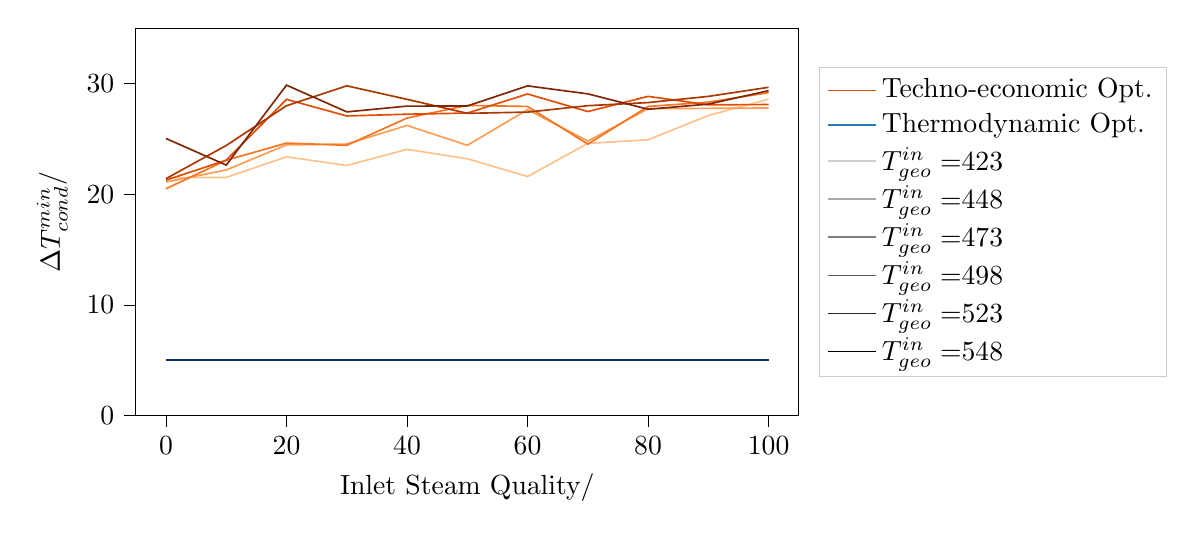
\begin{tikzpicture}

\definecolor{burlywood253194140}{RGB}{253,194,140}
\definecolor{chocolate24511733}{RGB}{245,117,33}
\definecolor{darkgray168}{RGB}{168,168,168}
\definecolor{darkgray176}{RGB}{176,176,176}
\definecolor{darkslategray41}{RGB}{41,41,41}
\definecolor{dimgray89}{RGB}{89,89,89}
\definecolor{gray127}{RGB}{127,127,127}
\definecolor{lightblue182212233}{RGB}{182,212,233}
\definecolor{lightgray204}{RGB}{204,204,204}
\definecolor{lightgray206}{RGB}{206,206,206}
\definecolor{midnightblue848107}{RGB}{8,48,107}
\definecolor{orangered222795}{RGB}{222,79,5}
\definecolor{saddlebrown127394}{RGB}{127,39,4}
\definecolor{saddlebrown171552}{RGB}{171,55,2}
\definecolor{sandybrown25315782}{RGB}{253,157,82}
\definecolor{skyblue131187219}{RGB}{131,187,219}
\definecolor{steelblue40120184}{RGB}{40,120,184}
\definecolor{steelblue80155203}{RGB}{80,155,203}
\definecolor{teal1084158}{RGB}{10,84,158}

\begin{axis}[
legend cell align={left},
legend style={
  fill opacity=0.8,
  draw opacity=1,
  text opacity=1,
  at={(1.03,0.5)},
  anchor=west,
  draw=lightgray204
},
tick align=outside,
tick pos=left,
x grid style={darkgray176},
xlabel={Inlet Steam Quality/\unit{\percent}},
xmin=-5, xmax=105,
xtick style={color=black},
y grid style={darkgray176},
ylabel={\(\Delta T_{cond}^{min}\)/\unit{\K}},
ymin=0, ymax=35,
ytick style={color=black},
width=10cm, height=6.5cm
]
\addplot [semithick, orangered222795]
table {%
0 -1
1 -1
};
\addlegendentry{Techno-economic Opt.}
\addplot [semithick, steelblue40120184]
table {%
0 -1
1 -1
};
\addlegendentry{Thermodynamic Opt.}
\addplot [semithick, lightgray206]
table {%
0 -1
1 -1
};
\addlegendentry{\(T_{geo}^{in}=\)\qty{423}{\K}}
\addplot [semithick, burlywood253194140, forget plot]
table {%
0 21.477693690657
10 21.516203103838
20 23.3776950121904
30 22.5939381327143
40 24.0531021944763
50 23.2025880174416
60 21.59941031362
70 24.5927744914032
80 24.9192024808735
90 27.1153552191322
100 28.5757311977719
};
\addplot [semithick, lightblue182212233, forget plot]
table {%
0 5
10 5
20 5
30 5
40 5
50 5
60 5
70 5
80 5
90 5
100 5
};
\addplot [semithick, darkgray168]
table {%
0 -1
1 -1
};
\addlegendentry{\(T_{geo}^{in}=\)\qty{448}{\K}}
\addplot [semithick, sandybrown25315782, forget plot]
table {%
0 21.1005872595034
10 22.1895163211857
20 24.4560746478686
30 24.5306942098682
40 26.2140837942385
50 24.4177148350573
60 27.6432915426399
70 24.8010573346589
80 27.7277120690675
90 27.7585803630629
100 27.7910844860225
};
\addplot [semithick, skyblue131187219, forget plot]
table {%
0 5
10 5
20 5
30 5
40 5
50 5
60 5
70 5
80 5
90 5
100 5
};
\addplot [semithick, gray127]
table {%
0 -1
1 -1
};
\addlegendentry{\(T_{geo}^{in}=\)\qty{473}{\K}}
\addplot [semithick, chocolate24511733, forget plot]
table {%
0 20.4899769126707
10 23.0688525352336
20 24.6197294934274
30 24.4177148350573
40 26.8809487432662
50 28.022670322494
60 27.931082697435
70 24.5241543075799
80 27.9275238192777
90 28.3209271291002
100 29.178323032567
};
\addplot [semithick, steelblue80155203, forget plot]
table {%
0 5
10 5
20 5
30 5
40 5
50 5
60 5
70 5
80 5
90 5
100 5
};
\addplot [semithick, dimgray89]
table {%
0 -1
1 -1
};
\addlegendentry{\(T_{geo}^{in}=\)\qty{498}{\K}}
\addplot [semithick, orangered222795, forget plot]
table {%
0 21.2688722310976
10 23.0719844000401
20 28.5713775512313
30 27.0703274918728
40 27.2298353506859
50 27.330702041515
60 29.056712917268
70 27.4676495547989
80 28.8407866227749
90 28.0792904190134
100 28.1017830769427
};
\addplot [semithick, steelblue40120184, forget plot]
table {%
0 5
10 5
20 5
30 5
40 5
50 5
60 5
70 5
80 5
90 5
100 5
};
\addplot [semithick, darkslategray41]
table {%
0 -1
1 -1
};
\addlegendentry{\(T_{geo}^{in}=\)\qty{523}{\K}}
\addplot [semithick, saddlebrown171552, forget plot]
table {%
0 21.4022921735182
10 24.4031776279197
20 27.9957652291495
30 29.7937737909401
40 28.5740034472093
50 27.307388008633
60 27.4188975700408
70 27.9991573926123
80 28.2806255438038
90 28.838797816093
100 29.6612520171413
};
\addplot [semithick, teal1084158, forget plot]
table {%
0 5
10 5
20 5
30 5
40 5
50 5
60 5
70 5
80 5
90 5
100 5
};
\addplot [semithick, black]
table {%
0 -1
1 -1
};
\addlegendentry{\(T_{geo}^{in}=\)\qty{548}{\K}}
\addplot [semithick, saddlebrown127394, forget plot]
table {%
0 25.035044694954
10 22.6286164997631
20 29.8554530172785
30 27.4389842257544
40 27.9613786274637
50 27.9681627613132
60 29.7893217104112
70 29.0673588298923
80 27.6780752995856
90 28.14074625524
100 29.3563569232359
};
\addplot [semithick, midnightblue848107, forget plot]
table {%
0 5
10 5
20 5
30 5
40 5
50 5
60 5
70 5
80 5
90 5
100 5
};
\end{axis}

\end{tikzpicture}

    %     \caption{The minimum approach temperature in the condenser \(T_{cond}^{min}\) for a techno-economically and a thermodynamically optimised single flash \ac{DSC} geothermal power plant.}
    %     \label{fig:prosim_purewater_DSC_techno_opt_DTpinch}
    % \end{figure}

    % \begin{figure}[H]
    %     \centering
    %     % This file was created with tikzplotlib v0.10.1.
\begin{tikzpicture}

\definecolor{burlywood253194140}{RGB}{253,194,140}
\definecolor{chocolate24511733}{RGB}{245,117,33}
\definecolor{darkgray168}{RGB}{168,168,168}
\definecolor{darkgray176}{RGB}{176,176,176}
\definecolor{darkslategray41}{RGB}{41,41,41}
\definecolor{dimgray89}{RGB}{89,89,89}
\definecolor{gray127}{RGB}{127,127,127}
\definecolor{lightblue182212233}{RGB}{182,212,233}
\definecolor{lightgray204}{RGB}{204,204,204}
\definecolor{lightgray206}{RGB}{206,206,206}
\definecolor{midnightblue848107}{RGB}{8,48,107}
\definecolor{orangered222795}{RGB}{222,79,5}
\definecolor{saddlebrown127394}{RGB}{127,39,4}
\definecolor{saddlebrown171552}{RGB}{171,55,2}
\definecolor{sandybrown25315782}{RGB}{253,157,82}
\definecolor{skyblue131187219}{RGB}{131,187,219}
\definecolor{steelblue40120184}{RGB}{40,120,184}
\definecolor{steelblue80155203}{RGB}{80,155,203}
\definecolor{teal1084158}{RGB}{10,84,158}

\begin{axis}[
legend cell align={left},
legend style={
  fill opacity=0.8,
  draw opacity=1,
  text opacity=1,
  at={(0.03,0.97)},
  anchor=north west,
  draw=lightgray204
},
log basis y={10},
tick align=outside,
tick pos=left,
x grid style={darkgray176},
xlabel={Inlet Steam Quality/\unit{\percent}},
xmin=-5, xmax=105,
xtick style={color=black},
y grid style={darkgray176},
ylabel={Condensation Pressure/\unit{\bar}},
ymin=0.08, ymax=1,
ymode=log,
ytick style={color=black},
ytick={0.001,0.01,0.1,1,10},
yticklabels={
  \(\displaystyle {10^{-3}}\),
  \(\displaystyle {10^{-2}}\),
  \(\displaystyle {10^{-1}}\),
  \(\displaystyle {10^{0}}\),
  \(\displaystyle {10^{1}}\)
}
]
\addplot [semithick, orangered222795]
table {%
0 0.01
1 0.01
};
\addlegendentry{Techno-economic Opt.}
\addplot [semithick, steelblue40120184]
table {%
0 0.01
1 0.01
};
\addlegendentry{Thermodynamic Opt.}
\addplot [semithick, lightgray206]
table {%
0 0.01
1 0.01
};
\addlegendentry{\(T_{geo}^{in}=\)\qty{423}{\K}}
\addplot [semithick, burlywood253194140, forget plot]
table {%
0 0.174087530100699
10 0.179924814092318
20 0.191028520165388
30 0.175800341628324
40 0.190242570275734
50 0.190211210886669
60 0.213592820065317
70 0.221635735978842
80 0.238725306724181
90 0.26427481641744
100 0.231780268129945
};
\addplot [semithick, lightblue182212233, forget plot]
table {%
0 0.100516491966174
10 0.10085891483133
20 0.100192045867075
30 0.100224882024193
40 0.100235163042185
50 0.100456267186974
60 0.100298468067612
70 0.100019683468695
80 0.100552445826177
90 0.100367889705308
100 0.101703752447466
};
\addplot [semithick, darkgray168]
table {%
0 0.01
1 0.01
};
\addlegendentry{\(T_{geo}^{in}=\)\qty{448}{\K}}
\addplot [semithick, sandybrown25315782, forget plot]
table {%
0 0.176247433450165
10 0.191371717927421
20 0.192756954730681
30 0.222926367856714
40 0.253958216620199
50 0.191371717927421
60 0.255801730589167
70 0.197677501032082
80 0.266807170011231
90 0.329412964191945
100 0.248176784962188
};
\addplot [semithick, skyblue131187219, forget plot]
table {%
0 0.100427505111133
10 0.100298519511268
20 0.100802699353455
30 0.100741003867798
40 0.100245627732832
50 0.100385680920635
60 0.100073305448595
70 0.10031374744751
80 0.10018924342083
90 0.100163248779866
100 0.100828199165435
};
\addplot [semithick, gray127]
table {%
0 0.01
1 0.01
};
\addlegendentry{\(T_{geo}^{in}=\)\qty{473}{\K}}
\addplot [semithick, chocolate24511733, forget plot]
table {%
0 0.168345370894104
10 0.192574965177159
20 0.235986118151431
30 0.262367931261817
40 0.228385938878899
50 0.260053708598205
60 0.30033000727183
70 0.239748996736392
80 0.285317892252238
90 0.295601392858194
100 0.350457434700946
};
\addplot [semithick, steelblue80155203, forget plot]
table {%
0 0.101777825050233
10 0.100084989109323
20 0.100275599880607
30 0.100594750538591
40 0.101191622080754
50 0.100038595400906
60 0.105528680012676
70 0.101151881995041
80 0.100594066365943
90 0.101345630716496
100 0.100464855786057
};
\addplot [semithick, dimgray89]
table {%
0 0.01
1 0.01
};
\addlegendentry{\(T_{geo}^{in}=\)\qty{498}{\K}}
\addplot [semithick, orangered222795, forget plot]
table {%
0 0.180056801692935
10 0.201970379280427
20 0.277771230742529
30 0.271324038156164
40 0.303931042880012
50 0.274186268854712
60 0.392991840098521
70 0.278637252067119
80 0.304817779923271
90 0.289948504939809
100 0.344617793309213
};
\addplot [semithick, steelblue40120184, forget plot]
table {%
0 0.100075621657955
10 0.100599011721345
20 0.100061467714184
30 0.100367682820982
40 0.100023572839883
50 0.100229732036354
60 0.100792351342826
70 0.100803498325385
80 0.100295265209646
90 0.100193863626635
100 0.102379512057631
};
\addplot [semithick, darkslategray41]
table {%
0 0.01
1 0.01
};
\addlegendentry{\(T_{geo}^{in}=\)\qty{523}{\K}}
\addplot [semithick, saddlebrown171552, forget plot]
table {%
0 0.184170191219056
10 0.191292384808462
20 0.297294679219482
30 0.345241155932278
40 0.355474241186701
50 0.262278682770742
60 0.270467807360662
70 0.313902515812438
80 0.361816384303774
90 0.294299906151366
100 0.335883059460169
};
\addplot [semithick, teal1084158, forget plot]
table {%
0 0.100664112501131
10 0.100725669665807
20 0.100490008736702
30 0.100277275370116
40 0.10045229035902
50 0.100108110826363
60 0.100141637623649
70 0.100439344052684
80 0.101215905538596
90 0.101255431363736
100 0.100186542305672
};
\addplot [semithick, black]
table {%
0 0.01
1 0.01
};
\addlegendentry{\(T_{geo}^{in}=\)\qty{548}{\K}}
\addplot [semithick, saddlebrown127394, forget plot]
table {%
0 0.20317544817479
10 0.207165598480273
20 0.281188563306618
30 0.241107217504802
40 0.26678469179397
50 0.301814539518751
60 0.319845281389624
70 0.314397413671355
80 0.314187822272418
90 0.350487430621055
100 0.38309688458165
};
\addplot [semithick, midnightblue848107, forget plot]
table {%
0 0.100456903580965
10 0.100415601521599
20 0.101440587576695
30 0.101903842312231
40 0.100941988080672
50 0.100022003475026
60 0.100269533130819
70 0.100726327650037
80 0.100655408129229
90 0.10139462330821
100 0.101648415540876
};
\end{axis}

\end{tikzpicture}

    %     \caption{The condensation pressure for a techno-economically and a thermodynamically optimised single flash \ac{DSC} geothermal power plant.}
    %     \label{fig:prosim_purewater_DSC_techno_opt_Pmin}
    % \end{figure}
    
    \begin{figure}[H]
        \centering
        \resizebox{\linewidth}{!}{% This file was created with tikzplotlib v0.10.1.
\begin{tikzpicture}

\definecolor{burlywood253194140}{RGB}{253,194,140}
\definecolor{chocolate24511733}{RGB}{245,117,33}
\definecolor{darkgray168}{RGB}{168,168,168}
\definecolor{darkgray176}{RGB}{176,176,176}
\definecolor{darkslategray41}{RGB}{41,41,41}
\definecolor{dimgray89}{RGB}{89,89,89}
\definecolor{gray127}{RGB}{127,127,127}
\definecolor{lightblue182212233}{RGB}{182,212,233}
\definecolor{lightgray204}{RGB}{204,204,204}
\definecolor{lightgray206}{RGB}{206,206,206}
\definecolor{midnightblue848107}{RGB}{8,48,107}
\definecolor{orangered222795}{RGB}{222,79,5}
\definecolor{saddlebrown127394}{RGB}{127,39,4}
\definecolor{saddlebrown171552}{RGB}{171,55,2}
\definecolor{sandybrown25315782}{RGB}{253,157,82}
\definecolor{skyblue131187219}{RGB}{131,187,219}
\definecolor{steelblue40120184}{RGB}{40,120,184}
\definecolor{steelblue80155203}{RGB}{80,155,203}
\definecolor{teal1084158}{RGB}{10,84,158}

\begin{groupplot}[
    group style={
        group size=2 by 3, 
        vertical sep=2.5cm, 
        horizontal sep=2.5cm},
    height=6cm, 
    width=7cm, 
]
\nextgroupplot[
legend cell align={left},
legend style={
  fill opacity=0.8,
  draw opacity=1,
  text opacity=1,
  at={(1.15,-0.35)},
  anchor=north,
  draw=lightgray204
},
legend columns=3
tick align=outside,
tick pos=left,
title={Techno-Economic Opt.},
x grid style={darkgray176},
xlabel={Inlet Steam Quality/\unit{\percent}},
xmin=-5, xmax=105,
xtick style={color=black},
y grid style={darkgray176},
ylabel={\(1-\frac{P_{flash}}{P_{geo}^{in}}\)/\unit{\percent}},
ymin=0, ymax=100,
ytick style={color=black}
]
\addplot [semithick, lightgray206]
table {%
0 -1
1 -1
};
\addlegendentry{\(T_{geo}^{in}=\)\qty{423}{\K}}
\addplot [semithick, burlywood253194140, forget plot]
table {%
0 48.8655923748958
10 1.27673416472691
20 2.01691736453029
30 1.14893035981736
40 1.67021018164867
50 1.87764169762544
60 2.15364683757056
70 3.4757072285431
80 1.86832437998504
90 1.1139266387809
100 1.31828855232208
};
\addplot [semithick, darkgray168]
table {%
0 -1
1 -1
};
\addlegendentry{\(T_{geo}^{in}=\)\qty{448}{\K}}
\addplot [semithick, sandybrown25315782, forget plot]
table {%
0 65.2100537980984
10 30.0004094873969
20 3.50288194229642
30 5.71800601142176
40 2.10674568068242
50 5.05862093783691
60 1.27089428796796
70 4.78287946534518
80 3.86299892483102
90 2.60897523578015
100 1.00040172795542
};
\addplot [semithick, gray127]
table {%
0 -1
1 -1
};
\addlegendentry{\(T_{geo}^{in}=\)\qty{473}{\K}}
\addplot [semithick, chocolate24511733, forget plot]
table {%
0 69.2196714410532
10 40.1575276804729
20 2.35637531392502
30 1.04514638115183
40 4.50982038531067
50 3.63903054778967
60 1.45510886558041
70 2.04827408298445
80 1.07118065877069
90 1.14886386035751
100 1.15389427038711
};
\addplot [semithick, dimgray89]
table {%
0 -1
1 -1
};
\addlegendentry{\(T_{geo}^{in}=\)\qty{498}{\K}}
\addplot [semithick, orangered222795, forget plot]
table {%
0 73.4164367124513
10 53.4655224762364
20 2.5603317643306
30 3.46105972108147
40 1.01086514943177
50 3.46597179345464
60 5.45277186224735
70 1.68609158314699
80 1.41801521528577
90 1.85543868187463
100 2.4154630844431
};
\addplot [semithick, darkslategray41]
table {%
0 -1
1 -1
};
\addlegendentry{\(T_{geo}^{in}=\)\qty{523}{\K}}
\addplot [semithick, saddlebrown171552, forget plot]
table {%
0 77.7388922969157
10 62.7776327491535
20 35.8138789516029
30 1.42892121799895
40 2.86115658776543
50 2.65855867264709
60 1.12566123351746
70 1.79764629875228
80 2.97322146606209
90 1.1517002469928
100 1.04230526139474
};
\addplot [semithick, black]
table {%
0 -1
1 -1
};
\addlegendentry{\(T_{geo}^{in}=\)\qty{548}{\K}}
\addplot [semithick, saddlebrown127394, forget plot]
table {%
0 80.6163901203627
10 69.5586428664754
20 45.7598815410276
30 10.9898990136667
40 3.75715454968593
50 1.73970607086177
60 1.93518113197584
70 1.17032279260463
80 2.92808934078091
90 1.2291493679313
100 1.40325218029683
};

\nextgroupplot[
tick align=outside,
tick pos=left,
title={Thermodynamic Opt.},
x grid style={darkgray176},
xlabel={Inlet Steam Quality/\unit{\percent}},
xmin=-5, xmax=105,
xtick style={color=black},
y grid style={darkgray176},
ylabel={\(1-\frac{P_{flash}}{P_{geo}^{in}}\)/\unit{\percent}},
ymin=0, ymax=100,
ytick style={color=black}
]
\addplot [semithick, lightblue182212233]
table {%
0 75.9553992271465
10 47.040006584378
20 6.19537876077439
30 1.23123396337197
40 1.19435940298285
50 1.26772820765488
60 1.18571701556611
70 1.0671695397221
80 1.13154959156995
90 1.33210202965343
100 1.08752011769148
};
\addplot [semithick, skyblue131187219]
table {%
0 80.7135897915828
10 62.0832098244219
20 32.850644473464
30 2.35294930171279
40 1.56013702024018
50 1.22629553228444
60 1.29572885174183
70 1.37148135928505
80 1.04227767364871
90 1.04238391278078
100 1.38946376838861
};
\addplot [semithick, steelblue80155203]
table {%
0 84.5242095937589
10 72.0402329565964
20 49.3377335134679
30 13.501848045413
40 1.5610804680803
50 1.14728241994362
60 1.73451597591555
70 1.20330128902574
80 1.04195945660294
90 1.33326235488206
100 1.03914219132547
};
\addplot [semithick, steelblue40120184]
table {%
0 85.7522101639238
10 77.7018539471498
20 60.439600051367
30 37.2873800634286
40 15.2857242748563
50 2.66582388697717
60 1.72506888865658
70 1.03761815241697
80 1.52076914113826
90 1.47881613895756
100 1.35712876596985
};
\addplot [semithick, teal1084158]
table {%
0 87.4625706053439
10 79.609433391719
20 70.6796906887176
30 57.0527181384922
40 37.9587873631251
50 10.9180989331347
60 1.97363947376031
70 1.21724721469586
80 1.45123541301602
90 1.43487511985059
100 1.22580664404766
};
\addplot [semithick, midnightblue848107]
table {%
0 88.3790988988582
10 82.4231630905649
20 74.2633407377298
30 65.8867157118041
40 51.221293652908
50 32.8154367955341
60 2.97218366096765
70 2.53237587959152
80 1.2581104957879
90 1.05331741021293
100 1.20352683086877
};
\end{groupplot}

\end{tikzpicture}
}
        \caption{The degree of flashing \(X_{flash}\) a techno-economically (left) and a thermodynamically (right) optimised single flash \ac{DSC} geothermal power plant.}
        \label{fig:prosim_purewater_DSC_techno_opt_Xflash}
    \end{figure}

\subsection{Performance Analysis: ORC}
    The techno-economic optimisation of the binary \ac{ORC} geothermal power plant reduces the specific plant cost by between about \qty{20}{\percent} to \qty{30}{\percent}, Figure~\ref{fig:prosim_purewater_Wnet_ORC_thermo_vs_techno}, at the expense of \qty{40}{\percent} to \qty{65}{\percent} of net electrical power, Figure~\ref{fig:prosim_purewater_SpecCost_ORC_thermo_vs_techno}. 
    \begin{figure}[H]
        \centering
        \resizebox{\linewidth}{!}{% This file was created with tikzplotlib v0.10.1.
\begin{tikzpicture}

\definecolor{chocolate2369815}{RGB}{236,98,15}
\definecolor{crimson2143940}{RGB}{214,39,40}
\definecolor{darkgray165}{RGB}{165,165,165}
\definecolor{darkgray176}{RGB}{176,176,176}
\definecolor{darkgreen06827}{RGB}{0,68,27}
\definecolor{darkorange25512714}{RGB}{255,127,14}
\definecolor{darkseagreen133204132}{RGB}{133,204,132}
\definecolor{darkslategray45}{RGB}{45,45,45}
\definecolor{dimgray108}{RGB}{108,108,108}
\definecolor{firebrick175572}{RGB}{175,57,2}
\definecolor{forestgreen4416044}{RGB}{44,160,44}
\definecolor{forestgreen611448}{RGB}{6,114,48}
\definecolor{gainsboro216}{RGB}{216,216,216}
\definecolor{lightgray198232191}{RGB}{198,232,191}
\definecolor{lightgray204}{RGB}{204,204,204}
\definecolor{lightgreen160216154}{RGB}{160,216,154}
\definecolor{mediumpurple148103189}{RGB}{148,103,189}
\definecolor{navajowhite253207161}{RGB}{253,207,161}
\definecolor{saddlebrown127394}{RGB}{127,39,4}
\definecolor{sandybrown25315378}{RGB}{253,153,78}
\definecolor{sandybrown253173106}{RGB}{253,173,106}
\definecolor{seagreen5816488}{RGB}{58,164,88}
\definecolor{sienna1408675}{RGB}{140,86,75}
\definecolor{silver188}{RGB}{188,188,188}
\definecolor{steelblue31119180}{RGB}{31,119,180}

\begin{groupplot}[
    group style={
        group size=2 by 3, 
        vertical sep=2.5cm, 
        horizontal sep=2.5cm},
    height=6cm, 
    width=7cm, 
]
\nextgroupplot[
legend cell align={left},
legend style={
  fill opacity=0.8,
  draw opacity=1,
  text opacity=1,
  at={(1.15,-0.35)},
  anchor=north,
  draw=lightgray204
},
legend columns=3,
tick align=outside,
tick pos=left,
x grid style={darkgray176},
xlabel={Inlet Steam Quality/\unit{\percent}},
xmin=-5, xmax=105,
xtick style={color=black},
y grid style={darkgray176},
ylabel={Specific Cost/\unit{\USD\of{2023}\per\kilo\watt}},
ymin=0, ymax=4121.03620848401,
ytick style={color=black}
]
\addplot [semithick, gainsboro216]
table {%
0 -1
1 -1
};
\addlegendentry{\(T_{geo}^{in}=\)\qty{423}{\K}}
\addplot [semithick, navajowhite253207161, forget plot]
table {%
0 3924.74876998477
10 2864.45589931569
20 2505.38785686709
30 2269.89381335059
40 2141.99269420881
50 2042.09967285358
60 1946.27753464857
70 1899.51219909746
80 1827.22934978168
100 1739.19911462868
};
\addplot [semithick, silver188]
table {%
0 -1
1 -1
};
\addlegendentry{\(T_{geo}^{in}=\)\qty{448}{\K}}
\addplot [semithick, sandybrown253173106, forget plot]
table {%
0 3121.71117657015
10 2406.06809173759
20 2107.01784237964
30 1929.20092397943
40 1819.42216592799
50 1718.7121447071
60 1657.84149154046
70 1596.26295036253
80 1542.8292558676
100 1463.56809441349
};
\addplot [semithick, darkgray165]
table {%
0 -1
1 -1
};
\addlegendentry{\(T_{geo}^{in}=\)\qty{473}{\K}}
\addplot [semithick, sandybrown25315378, forget plot]
table {%
0 2625.2265999825
10 2145.05130794449
20 1893.74166250286
30 1782.13037671762
40 1674.71105037335
50 1587.89848380553
60 1487.75793090714
70 1441.39829920263
80 1427.97710681161
100 1325.36906819417
};
\addplot [semithick, dimgray108]
table {%
0 -1
1 -1
};
\addlegendentry{\(T_{geo}^{in}=\)\qty{498}{\K}}
\addplot [semithick, chocolate2369815, forget plot]
table {%
0 2262.03270107405
10 2020.58462764707
20 1816.3157104373
30 1742.05751609993
40 1564.73764758435
50 1522.07798250182
60 1434.53880608932
70 1379.31503816859
80 1334.71528741857
100 1288.80327344859
};
\addplot [semithick, darkslategray45]
table {%
0 -1
1 -1
};
\addlegendentry{\(T_{geo}^{in}=\)\qty{523}{\K}}
\addplot [semithick, firebrick175572, forget plot]
table {%
0 2090.08535835198
10 1892.68127999503
20 1742.17921155996
30 1622.83845995606
40 1514.16724155544
50 1452.06053559895
60 1383.3251196894
70 1335.35027058075
80 1294.98002490666
100 1220.93724373735
};
\addplot [semithick, black]
table {%
0 -1
1 -1
};
\addlegendentry{\(T_{geo}^{in}=\)\qty{548}{\K}}
\addplot [semithick, saddlebrown127394, forget plot]
table {%
0 1957.04090182849
10 1738.82345776563
20 1616.26252861641
30 1542.81948667963
40 1455.43757331271
50 1392.0701307236
60 1330.19220729471
70 1285.26488993122
80 1241.74951039109
100 1173.97094076806
};

\nextgroupplot[
tick align=outside,
tick pos=left,
x grid style={darkgray176},
xlabel={Inlet Steam Quality/\unit{\percent}},
xmin=-5, xmax=105,
xtick style={color=black},
y grid style={darkgray176},
ylabel={Delta Specific Cost/\unit{\USD\of{2023}\per\kilo\watt}},
ymin=-1288.80024602716, ymax=0,
ytick style={color=black},
ytick distance=250
]
\addplot [semithick, steelblue31119180, draw=none]
table {%
0 -919.337171956103
100 -192.262687922356
};
\addplot [semithick, darkorange25512714, draw=none]
table {%
0 -1236.5841718317
100 -414.749228956379
};
\addplot [semithick, forestgreen4416044, draw=none]
table {%
0 -959.82246526439
100 -452.182515436185
};
\addplot [semithick, crimson2143940, draw=none]
table {%
0 -1229.65582471511
100 -457.145808852914
};
\addplot [semithick, mediumpurple148103189, draw=none]
table {%
0 -837.290068554075
100 -509.398947897534
};
\addplot [semithick, sienna1408675, draw=none]
table {%
0 -673.964514822544
100 -499.230358259416
};
\end{groupplot}

\begin{groupplot}[
    group style={
        group size=2 by 3, 
        vertical sep=2.5cm, 
        horizontal sep=2.5cm},
    height=6cm, 
    width=7cm, 
]
\nextgroupplot[
axis x line= none,
axis y line=none,
xmajorticks=false,
ymajorticks=false
]
\nextgroupplot[
axis y line=right,
tick align=outside,
x grid style={darkgray176},
xmin=-5, xmax=105,
xtick pos=left,
xtick style={color=black},
y grid style={darkgray176},
ylabel={Delta Specific Cost/\unit{\percent}},
ymin=-36.743987553777, ymax=0,
ytick pos=right,
ytick style={color=black},
yticklabel style={anchor=west}
]
\addplot [semithick, lightgray198232191]
table {%
0 -4.66995756237445
10 -24.2967084784871
20 -23.5524779552772
30 -21.3434838119786
40 -19.3795511382771
50 -19.5067115994913
60 -18.9024086245842
70 -18.1010405388953
80 -19.0262474428587
100 -19.3235130189168
};
\addplot [semithick, lightgreen160216154]
table {%
0 -22.5274630188885
10 -33.9473571001811
20 -26.5573344300375
30 -22.5020725409645
40 -21.1014335865908
50 -21.6726604154279
60 -21.3024558062308
70 -21.7292947270982
80 -22.2221124468358
100 -22.0808924986265
};
\addplot [semithick, darkseagreen133204132]
table {%
0 -26.7729241021779
10 -29.967816794459
20 -27.1966187191474
30 -24.7873448903543
40 -23.29876649331
50 -23.9576013727118
60 -25.2304830507662
70 -25.592022476806
80 -24.0502194646424
100 -25.7254721675003
};
\addplot [semithick, seagreen5816488]
table {%
0 -35.2166527922817
10 -27.9995226174436
20 -25.5909181461337
30 -22.8647404011439
40 -27.2469500725241
50 -25.1852301922399
60 -26.6362065160344
70 -28.5063532959662
80 -27.7734772106816
100 -26.1832268470457
};
\addplot [semithick, forestgreen611448]
table {%
0 -28.6020734087738
10 -25.7206515234946
20 -25.7174693858864
30 -26.0896885917308
40 -26.6668283747315
50 -26.9361660521047
60 -27.6867087731992
70 -28.0932343128763
80 -28.5948352481351
100 -29.4393049373969
};
\addplot [semithick, darkgreen06827]
table {%
0 -25.6162344082295
10 -27.4013437437694
20 -26.8633004238702
30 -27.9443548450381
40 -29.645857051911
50 -29.6094391888003
60 -29.7999837151933
70 -29.6046621548943
80 -30.2164224635348
100 -29.8368378359248
};
\end{groupplot}

\end{tikzpicture}
}
        \caption[The minimum specific cost of the techno-economically optimised  binary \ac{ORC}.]{Left: the minimum specific cost of the techno-economically optimised  binary \ac{ORC}. Right: the difference to the minimum specific cost obtained for the thermodynamically optimised binary \ac{ORC}.}
        \label{fig:prosim_purewater_Wnet_ORC_thermo_vs_techno}
    \end{figure}

    \begin{figure}[H]
        \centering
        \resizebox{\linewidth}{!}{% This file was created with tikzplotlib v0.10.1.
\begin{tikzpicture}

\definecolor{chocolate2369815}{RGB}{236,98,15}
\definecolor{crimson2143940}{RGB}{214,39,40}
\definecolor{darkgray165}{RGB}{165,165,165}
\definecolor{darkgray176}{RGB}{176,176,176}
\definecolor{darkgreen06827}{RGB}{0,68,27}
\definecolor{darkorange25512714}{RGB}{255,127,14}
\definecolor{darkseagreen133204132}{RGB}{133,204,132}
\definecolor{darkslategray45}{RGB}{45,45,45}
\definecolor{dimgray108}{RGB}{108,108,108}
\definecolor{firebrick175572}{RGB}{175,57,2}
\definecolor{forestgreen4416044}{RGB}{44,160,44}
\definecolor{forestgreen611448}{RGB}{6,114,48}
\definecolor{gainsboro216}{RGB}{216,216,216}
\definecolor{lightgray198232191}{RGB}{198,232,191}
\definecolor{lightgray204}{RGB}{204,204,204}
\definecolor{lightgreen160216154}{RGB}{160,216,154}
\definecolor{mediumpurple148103189}{RGB}{148,103,189}
\definecolor{navajowhite253207161}{RGB}{253,207,161}
\definecolor{saddlebrown127394}{RGB}{127,39,4}
\definecolor{sandybrown25315378}{RGB}{253,153,78}
\definecolor{sandybrown253173106}{RGB}{253,173,106}
\definecolor{seagreen5816488}{RGB}{58,164,88}
\definecolor{sienna1408675}{RGB}{140,86,75}
\definecolor{silver188}{RGB}{188,188,188}
\definecolor{steelblue31119180}{RGB}{31,119,180}

\begin{groupplot}[group style={group size=1 by 2}]
\nextgroupplot[
legend cell align={left},
legend style={
  fill opacity=0.8,
  draw opacity=1,
  text opacity=1,
  at={(0.03,0.97)},
  anchor=north west,
  draw=lightgray204
},
tick align=outside,
tick pos=left,
x grid style={darkgray176},
xlabel={Inlet Steam Quality/\unit{\percent}},
xmin=-5, xmax=105,
xtick style={color=black},
y grid style={darkgray176},
ylabel={Net electric power/\unit{\mega\watt}},
ymin=0, ymax=27.5872839351855,
ytick style={color=black}
]
\addplot [semithick, gainsboro216]
table {%
0 -1
1 -1
};
\addlegendentry{\(T_{geo}^{in}=\)\qty{423}{\K}}
\addplot [semithick, navajowhite253207161, forget plot]
table {%
0 0.557114149477613
10 1.638809379093
20 3.21412473778287
30 4.88993046912543
40 6.40119018667188
50 8.01183196896339
60 9.44767830676006
70 10.8199603723257
80 12.2488536362307
90 13.4670866211045
100 15.2483801805043
};
\addplot [semithick, silver188]
table {%
0 -1
1 -1
};
\addlegendentry{\(T_{geo}^{in}=\)\qty{448}{\K}}
\addplot [semithick, sandybrown253173106, forget plot]
table {%
0 1.08066458863151
10 2.2510134932247
20 3.92997004383771
30 5.74272006643475
40 7.49889052798885
50 9.71407527195079
60 11.2066841203576
70 13.5069457281367
80 14.7331560417993
90 16.0484312745728
100 18.7500172587311
};
\addplot [semithick, darkgray165]
table {%
0 -1
1 -1
};
\addlegendentry{\(T_{geo}^{in}=\)\qty{473}{\K}}
\addplot [semithick, sandybrown25315378, forget plot]
table {%
0 1.64052050679576
10 2.87437434461262
20 4.43651027514178
30 6.54064816254777
40 8.79912360916101
50 10.7969730793877
60 12.751824036599
70 15.3704403856425
80 17.1222600178921
90 19.1540821291431
100 20.7412826958224
};
\addplot [semithick, dimgray108]
table {%
0 -1
1 -1
};
\addlegendentry{\(T_{geo}^{in}=\)\qty{498}{\K}}
\addplot [semithick, chocolate2369815, forget plot]
table {%
0 2.30555058647817
10 3.65977973139912
20 4.83127169874635
30 7.24894705666434
40 9.50696724488665
50 11.9924728626009
60 13.6748087725596
70 16.757977411243
80 18.9233907014631
90 21.4106157835453
100 23.2626803222292
};
\addplot [semithick, darkslategray45]
table {%
0 -1
1 -1
};
\addlegendentry{\(T_{geo}^{in}=\)\qty{523}{\K}}
\addplot [semithick, firebrick175572, forget plot]
table {%
0 3.14394468871166
10 4.57715473188939
20 5.88207130807426
30 7.59483919695904
40 10.0956998814759
50 13.0154460785487
60 15.5655359107965
70 17.8582574715776
80 20.0412390531391
90 23.0908760896533
100 25.2823359007929
};
\addplot [semithick, black]
table {%
0 -1
1 -1
};
\addlegendentry{\(T_{geo}^{in}=\)\qty{548}{\K}}
\addplot [semithick, saddlebrown127394, forget plot]
table {%
0 4.04694608432612
10 5.56385477936918
20 6.78431620199085
30 8.51801675553119
40 10.9574501504885
50 13.4872385647876
60 16.0443522656724
70 18.7578315602252
80 21.4234178239481
90 23.8643640354297
100 26.2259847001766
};

\nextgroupplot[
tick align=outside,
tick pos=left,
x grid style={darkgray176},
xlabel={Inlet Steam Quality/\unit{\percent}},
xmin=-5, xmax=105,
xtick style={color=black},
y grid style={darkgray176},
ylabel={Delta net electric power/\unit{\mega\watt}},
ymin=-3.93280791519094, ymax=0,
ytick style={color=black}
]
\addplot [semithick, steelblue31119180]
table {%
0 -2.84601047168316
100 -0.291652185834188
};
\addplot [semithick, darkorange25512714]
table {%
0 -3.40523806870981
100 -0.292324648561037
};
\addplot [semithick, forestgreen4416044]
table {%
0 -3.75941954712633
100 -0.366529256377018
};
\addplot [semithick, crimson2143940]
table {%
0 -3.52764411093916
100 -0.466485654722207
};
\addplot [semithick, mediumpurple148103189]
table {%
0 -3.32980391887508
100 -0.508783358156812
};
\addplot [semithick, sienna1408675]
table {%
0 -3.53077922930065
100 -0.633244379239026
};
\end{groupplot}

\begin{groupplot}[group style={group size=1 by 2}]
\nextgroupplot[
axis y line=right,
tick align=outside,
x grid style={darkgray176},
xmin=-5, xmax=105,
xtick pos=left,
xtick style={color=black},
y grid style={darkgray176},
ylabel={Delta net electric power/\unit{\percent}},
ymin=-35.6182209348513, ymax=0,
ytick pos=right,
ytick style={color=black},
yticklabel style={anchor=west}
]
\addplot [semithick, lightgray198232191]
table {%
0 -34.3618936921016
10 -19.2569173809202
20 -11.6216920007034
30 -10.2490740191813
40 -11.820915657089
50 -11.630320421425
60 -13.1672336069283
70 -14.7978453432296
80 -15.5228106473986
90 -17.401388022819
100 -15.7286892186065
};
\addplot [semithick, lightgreen160216154]
table {%
0 -21.2911099841375
10 -17.1173479495208
20 -11.3311559613124
30 -11.5406631013656
40 -13.327295275599
50 -10.1492879249782
60 -13.6026127687655
70 -10.6867976092452
80 -14.8075212120392
90 -17.5043484528313
100 -13.0978235075709
};
\addplot [semithick, darkseagreen133204132]
table {%
0 -18.2620911101678
10 -17.5504322631739
20 -16.1451651140697
30 -11.6848274317958
40 -10.3105790534007
50 -11.99598401952
60 -12.9152958426412
70 -10.3653226264698
80 -12.6725511672419
90 -13.0532984177156
100 -15.3441297716611
};
\addplot [semithick, seagreen5816488]
table {%
0 -16.8282668093908
10 -15.6657199688942
20 -22.1288501541303
30 -13.1185294481165
40 -11.813057618197
50 -10.7187913626876
60 -15.0985074125849
70 -10.8406409235639
80 -11.8569508668125
90 -11.3404091870634
100 -13.1676050424073
};
\addplot [semithick, forestgreen611448]
table {%
0 -13.9288595161909
10 -13.4355100879494
20 -18.0032839138904
30 -18.3850473478656
40 -13.6149567902455
50 -9.235348837108
60 -9.42134569740691
70 -10.8960102511941
80 -12.4105780522798
90 -10.2666944072584
100 -11.6377311863483
};
\addplot [semithick, darkgreen06827]
table {%
0 -13.5303121564982
10 -12.2125205692685
20 -17.230366623561
30 -17.0311661493831
40 -12.8006228058856
50 -10.6783537777951
60 -10.3476267051903
70 -10.029630596816
80 -10.1052381371849
90 -10.9413072817334
100 -11.8654677560655
};
\end{groupplot}

\end{tikzpicture}
}
        \caption[The maximum net electrical power of the techno-economically optimised  binary \ac{ORC}.]{Left: the maximum net electrical power of the techno-economically optimised  binary \ac{ORC}. Right: the difference to the maximum net electrical power obtained for the thermodynamically optimised binary \ac{ORC}.}
        \label{fig:prosim_purewater_SpecCost_ORC_thermo_vs_techno}
    \end{figure}

    The reduction in specific plant cost is primarily driven by the miniaturisation of the turbine and the condenser, Figure~\ref{fig:prosim_purewater_ORC_techno_Costbreakdown}. The cost of the condenser is reduced irrespective of working fluid, while the cost of the turbine is only reduced for heavier more complex working fluids like Isopentane or n-Heptane.

    \begin{figure}[H]
        \centering
        % This file was created with tikzplotlib v0.10.1.
\begin{tikzpicture}

\definecolor{crimson2143940}{RGB}{214,39,40}
\definecolor{darkgray176}{RGB}{176,176,176}
\definecolor{darkorange25512714}{RGB}{255,127,14}
\definecolor{forestgreen4416044}{RGB}{44,160,44}
\definecolor{lightgray204}{RGB}{204,204,204}
\definecolor{mediumpurple148103189}{RGB}{148,103,189}
\definecolor{sienna1408675}{RGB}{140,86,75}
\definecolor{steelblue31119180}{RGB}{31,119,180}

\begin{groupplot}[
    group style={
        group size=2 by 3, 
        vertical sep=2.5cm, 
        horizontal sep=2.5cm},
    height=6cm, 
    width=6.5cm, 
    legend cell align={left},
    legend style={
        fill opacity=0.8,
        draw opacity=1,
        text opacity=1,
        draw=lightgray204,
        at={(1.25, 1.3)},
        anchor= south},
    legend columns=3
]
\nextgroupplot[
legend cell align={left},
tick align=outside,
tick pos=left,
title={n-Propane: Techno-Economic Opt.},
x grid style={darkgray176},
xlabel={Steam Quality/\unit{\percent}},
xmin=-7.75, xmax=107.75,
xtick style={color=black},
y grid style={darkgray176},
ylabel={Cost/\unit{\mega\USD\of{2023}}},
ymin=0, ymax=25,
ytick style={color=black},
ytick distance=5
]
\draw[draw=none,fill=steelblue31119180] (axis cs:-2.5,0) rectangle (axis cs:2.5,1.09806963284397);
\addlegendimage{ybar,area legend,draw=none,fill=steelblue31119180}
\addlegendentry{Turbine}

\draw[draw=none,fill=steelblue31119180] (axis cs:7.5,0) rectangle (axis cs:12.5,1.26530378524128);
\draw[draw=none,fill=steelblue31119180] (axis cs:17.5,0) rectangle (axis cs:22.5,1.40028192728012);
\draw[draw=none,fill=steelblue31119180] (axis cs:27.5,0) rectangle (axis cs:32.5,1.54827553312375);
\draw[draw=none,fill=steelblue31119180] (axis cs:37.5,0) rectangle (axis cs:42.5,1.66600683645384);
\draw[draw=none,fill=steelblue31119180] (axis cs:47.5,0) rectangle (axis cs:52.5,1.80586427313009);
\draw[draw=none,fill=steelblue31119180] (axis cs:57.5,0) rectangle (axis cs:62.5,1.9323981589596);
\draw[draw=none,fill=steelblue31119180] (axis cs:67.5,0) rectangle (axis cs:72.5,2.02107190036164);
\draw[draw=none,fill=steelblue31119180] (axis cs:77.5,0) rectangle (axis cs:82.5,2.12142629923048);
\draw[draw=none,fill=steelblue31119180] (axis cs:97.5,0) rectangle (axis cs:102.5,2.34999603027922);
\draw[draw=none,fill=darkorange25512714] (axis cs:-2.5,1.09806963284397) rectangle (axis cs:2.5,2.45857315348023);
\addlegendimage{ybar,area legend,draw=none,fill=darkorange25512714}
\addlegendentry{Condenser}

\draw[draw=none,fill=darkorange25512714] (axis cs:7.5,1.26530378524128) rectangle (axis cs:12.5,2.93581071720844);
\draw[draw=none,fill=darkorange25512714] (axis cs:17.5,1.40028192728012) rectangle (axis cs:22.5,3.3503555383725);
\draw[draw=none,fill=darkorange25512714] (axis cs:27.5,1.54827553312375) rectangle (axis cs:32.5,3.84049998355439);
\draw[draw=none,fill=darkorange25512714] (axis cs:37.5,1.66600683645384) rectangle (axis cs:42.5,4.03208447550348);
\draw[draw=none,fill=darkorange25512714] (axis cs:47.5,1.80586427313009) rectangle (axis cs:52.5,4.85947624598491);
\draw[draw=none,fill=darkorange25512714] (axis cs:57.5,1.9323981589596) rectangle (axis cs:62.5,5.20482863078829);
\draw[draw=none,fill=darkorange25512714] (axis cs:67.5,2.02107190036164) rectangle (axis cs:72.5,5.23476197725251);
\draw[draw=none,fill=darkorange25512714] (axis cs:77.5,2.12142629923048) rectangle (axis cs:82.5,5.51153531025739);
\draw[draw=none,fill=darkorange25512714] (axis cs:97.5,2.34999603027922) rectangle (axis cs:102.5,6.4593372311355);
\draw[draw=none,fill=forestgreen4416044] (axis cs:-2.5,2.45857315348023) rectangle (axis cs:2.5,3.64430621960449);
\addlegendimage{ybar,area legend,draw=none,fill=forestgreen4416044}
\addlegendentry{Other Equipment}

\draw[draw=none,fill=forestgreen4416044] (axis cs:7.5,2.93581071720844) rectangle (axis cs:12.5,4.32195201636134);
\draw[draw=none,fill=forestgreen4416044] (axis cs:17.5,3.3503555383725) rectangle (axis cs:22.5,4.90514560677214);
\draw[draw=none,fill=forestgreen4416044] (axis cs:27.5,3.84049998355439) rectangle (axis cs:32.5,5.60722864983634);
\draw[draw=none,fill=forestgreen4416044] (axis cs:37.5,4.03208447550348) rectangle (axis cs:42.5,5.89280657829721);
\draw[draw=none,fill=forestgreen4416044] (axis cs:47.5,4.85947624598491) rectangle (axis cs:52.5,7.06673325018463);
\draw[draw=none,fill=forestgreen4416044] (axis cs:57.5,5.20482863078829) rectangle (axis cs:62.5,7.57143647401275);
\draw[draw=none,fill=forestgreen4416044] (axis cs:67.5,5.23476197725251) rectangle (axis cs:72.5,7.62475183786065);
\draw[draw=none,fill=forestgreen4416044] (axis cs:77.5,5.51153531025739) rectangle (axis cs:82.5,8.02440830566714);
\draw[draw=none,fill=forestgreen4416044] (axis cs:97.5,6.4593372311355) rectangle (axis cs:102.5,9.39613635765176);
\draw[draw=none,fill=crimson2143940] (axis cs:-2.5,3.64430621960449) rectangle (axis cs:2.5,4.09917174724593);
\addlegendimage{ybar,area legend,draw=none,fill=crimson2143940}
\addlegendentry{PHE}

\draw[draw=none,fill=crimson2143940] (axis cs:7.5,4.32195201636134) rectangle (axis cs:12.5,4.79143763487817);
\draw[draw=none,fill=crimson2143940] (axis cs:17.5,4.90514560677214) rectangle (axis cs:22.5,5.3743596254263);
\draw[draw=none,fill=crimson2143940] (axis cs:27.5,5.60722864983634) rectangle (axis cs:32.5,6.10777136685818);
\draw[draw=none,fill=crimson2143940] (axis cs:37.5,5.89280657829721) rectangle (axis cs:42.5,6.42981651628164);
\draw[draw=none,fill=crimson2143940] (axis cs:47.5,7.06673325018463) rectangle (axis cs:52.5,7.63463688935893);
\draw[draw=none,fill=crimson2143940] (axis cs:57.5,7.57143647401275) rectangle (axis cs:62.5,8.18470258375979);
\draw[draw=none,fill=crimson2143940] (axis cs:67.5,7.62475183786065) rectangle (axis cs:72.5,8.26145243998036);
\draw[draw=none,fill=crimson2143940] (axis cs:77.5,8.02440830566714) rectangle (axis cs:82.5,8.68558529509994);
\draw[draw=none,fill=crimson2143940] (axis cs:97.5,9.39613635765176) rectangle (axis cs:102.5,10.1555349388163);
\draw[draw=none,fill=mediumpurple148103189] (axis cs:-2.5,4.09917174724593) rectangle (axis cs:2.5,4.15006573143491);
\addlegendimage{ybar,area legend,draw=none,fill=mediumpurple148103189}
\addlegendentry{Pump}

\draw[draw=none,fill=mediumpurple148103189] (axis cs:7.5,4.79143763487817) rectangle (axis cs:12.5,4.85149454703514);
\draw[draw=none,fill=mediumpurple148103189] (axis cs:17.5,5.3743596254263) rectangle (axis cs:22.5,5.44176523939873);
\draw[draw=none,fill=mediumpurple148103189] (axis cs:27.5,6.10777136685818) rectangle (axis cs:32.5,6.18355033198683);
\draw[draw=none,fill=mediumpurple148103189] (axis cs:37.5,6.42981651628164) rectangle (axis cs:42.5,6.51252735977806);
\draw[draw=none,fill=mediumpurple148103189] (axis cs:47.5,7.63463688935893) rectangle (axis cs:52.5,7.72539951469903);
\draw[draw=none,fill=mediumpurple148103189] (axis cs:57.5,8.18470258375979) rectangle (axis cs:62.5,8.28312745128564);
\draw[draw=none,fill=mediumpurple148103189] (axis cs:67.5,8.26145243998036) rectangle (axis cs:72.5,8.36496451212848);
\draw[draw=none,fill=mediumpurple148103189] (axis cs:77.5,8.68558529509994) rectangle (axis cs:82.5,8.79505548393412);
\draw[draw=none,fill=mediumpurple148103189] (axis cs:97.5,10.1555349388163) rectangle (axis cs:102.5,10.2787969428069);
\draw[draw=none,fill=sienna1408675] (axis cs:-2.5,4.15006573143491) rectangle (axis cs:2.5,7.05511174343934);
\addlegendimage{ybar,area legend,draw=none,fill=sienna1408675}
\addlegendentry{Construction}

\draw[draw=none,fill=sienna1408675] (axis cs:7.5,4.85149454703514) rectangle (axis cs:12.5,8.24754072995973);
\draw[draw=none,fill=sienna1408675] (axis cs:17.5,5.44176523939873) rectangle (axis cs:22.5,9.25100090697785);
\draw[draw=none,fill=sienna1408675] (axis cs:27.5,6.18355033198683) rectangle (axis cs:32.5,10.5120355643776);
\draw[draw=none,fill=sienna1408675] (axis cs:37.5,6.51252735977806) rectangle (axis cs:42.5,11.0712965116227);
\draw[draw=none,fill=sienna1408675] (axis cs:47.5,7.72539951469903) rectangle (axis cs:52.5,13.1331791749883);
\draw[draw=none,fill=sienna1408675] (axis cs:57.5,8.28312745128564) rectangle (axis cs:62.5,14.0813166671856);
\draw[draw=none,fill=sienna1408675] (axis cs:67.5,8.36496451212848) rectangle (axis cs:72.5,14.2204396706184);
\draw[draw=none,fill=sienna1408675] (axis cs:77.5,8.79505548393412) rectangle (axis cs:82.5,14.951594322688);
\draw[draw=none,fill=sienna1408675] (axis cs:97.5,10.2787969428069) rectangle (axis cs:102.5,17.4739548027718);

\nextgroupplot[
tick align=outside,
tick pos=left,
title={n-Propane: Thermodynamic Opt.},
x grid style={darkgray176},
xlabel={Steam Quality/\unit{\percent}},
xmin=-7.75, xmax=107.75,
xtick style={color=black},
y grid style={darkgray176},
ylabel={Cost/\unit{\mega\USD\of{2023}}},
ymin=0, ymax=25,
ytick style={color=black},
ytick distance=5
]
\draw[draw=none,fill=steelblue31119180] (axis cs:-2.5,0) rectangle (axis cs:2.5,1.23411541695185);
\draw[draw=none,fill=steelblue31119180] (axis cs:7.5,0) rectangle (axis cs:12.5,1.3864814498535);
\draw[draw=none,fill=steelblue31119180] (axis cs:17.5,0) rectangle (axis cs:22.5,1.52938044726175);
\draw[draw=none,fill=steelblue31119180] (axis cs:27.5,0) rectangle (axis cs:32.5,1.66583302812863);
\draw[draw=none,fill=steelblue31119180] (axis cs:37.5,0) rectangle (axis cs:42.5,1.79400584882137);
\draw[draw=none,fill=steelblue31119180] (axis cs:47.5,0) rectangle (axis cs:52.5,1.91748933410088);
\draw[draw=none,fill=steelblue31119180] (axis cs:57.5,0) rectangle (axis cs:62.5,2.03254339641068);
\draw[draw=none,fill=steelblue31119180] (axis cs:67.5,0) rectangle (axis cs:72.5,2.14179745195344);
\draw[draw=none,fill=steelblue31119180] (axis cs:77.5,0) rectangle (axis cs:82.5,2.25335327021377);
\draw[draw=none,fill=steelblue31119180] (axis cs:87.5,0) rectangle (axis cs:92.5,2.3631911957944);
\draw[draw=none,fill=steelblue31119180] (axis cs:97.5,0) rectangle (axis cs:102.5,2.4575976272655);
\draw[draw=none,fill=darkorange25512714] (axis cs:-2.5,1.23411541695185) rectangle (axis cs:2.5,3.47533273022563);
\draw[draw=none,fill=darkorange25512714] (axis cs:7.5,1.3864814498535) rectangle (axis cs:12.5,4.0078837358027);
\draw[draw=none,fill=darkorange25512714] (axis cs:17.5,1.52938044726175) rectangle (axis cs:22.5,4.5395224379318);
\draw[draw=none,fill=darkorange25512714] (axis cs:27.5,1.66583302812863) rectangle (axis cs:32.5,5.08331686850128);
\draw[draw=none,fill=darkorange25512714] (axis cs:37.5,1.79400584882137) rectangle (axis cs:42.5,5.59885811997817);
\draw[draw=none,fill=darkorange25512714] (axis cs:47.5,1.91748933410088) rectangle (axis cs:52.5,6.11935206004068);
\draw[draw=none,fill=darkorange25512714] (axis cs:57.5,2.03254339641068) rectangle (axis cs:62.5,6.6055187888777);
\draw[draw=none,fill=darkorange25512714] (axis cs:67.5,2.14179745195344) rectangle (axis cs:72.5,7.04894295150115);
\draw[draw=none,fill=darkorange25512714] (axis cs:77.5,2.25335327021377) rectangle (axis cs:82.5,7.5911085332406);
\draw[draw=none,fill=darkorange25512714] (axis cs:87.5,2.3631911957944) rectangle (axis cs:92.5,8.15017716733619);
\draw[draw=none,fill=darkorange25512714] (axis cs:97.5,2.4575976272655) rectangle (axis cs:102.5,8.50378831540512);
\draw[draw=none,fill=forestgreen4416044] (axis cs:-2.5,3.47533273022563) rectangle (axis cs:2.5,5.26832693037256);
\draw[draw=none,fill=forestgreen4416044] (axis cs:7.5,4.0078837358027) rectangle (axis cs:12.5,5.98575970144018);
\draw[draw=none,fill=forestgreen4416044] (axis cs:17.5,4.5395224379318) rectangle (axis cs:22.5,6.72335045014837);
\draw[draw=none,fill=forestgreen4416044] (axis cs:27.5,5.08331686850128) rectangle (axis cs:32.5,7.48700477918955);
\draw[draw=none,fill=forestgreen4416044] (axis cs:37.5,5.59885811997818) rectangle (axis cs:42.5,8.21531969375626);
\draw[draw=none,fill=forestgreen4416044] (axis cs:47.5,6.11935206004068) rectangle (axis cs:52.5,8.95338993354969);
\draw[draw=none,fill=forestgreen4416044] (axis cs:57.5,6.6055187888777) rectangle (axis cs:62.5,9.64554864160387);
\draw[draw=none,fill=forestgreen4416044] (axis cs:67.5,7.04894295150115) rectangle (axis cs:72.5,10.2784235232394);
\draw[draw=none,fill=forestgreen4416044] (axis cs:77.5,7.5911085332406) rectangle (axis cs:82.5,11.0513157724679);
\draw[draw=none,fill=forestgreen4416044] (axis cs:87.5,8.15017716733619) rectangle (axis cs:92.5,11.8483165184431);
\draw[draw=none,fill=forestgreen4416044] (axis cs:97.5,8.50378831540512) rectangle (axis cs:102.5,12.3570972428124);
\draw[draw=none,fill=crimson2143940] (axis cs:-2.5,5.26832693037256) rectangle (axis cs:2.5,6.21739789058035);
\draw[draw=none,fill=crimson2143940] (axis cs:7.5,5.98575970144018) rectangle (axis cs:12.5,6.85598675939002);
\draw[draw=none,fill=crimson2143940] (axis cs:17.5,6.72335045014837) rectangle (axis cs:22.5,7.56875764700185);
\draw[draw=none,fill=crimson2143940] (axis cs:27.5,7.48700477918955) rectangle (axis cs:32.5,8.3304665836589);
\draw[draw=none,fill=crimson2143940] (axis cs:37.5,8.21531969375626) rectangle (axis cs:42.5,9.06776847095174);
\draw[draw=none,fill=crimson2143940] (axis cs:47.5,8.95338993354969) rectangle (axis cs:52.5,9.82192011489636);
\draw[draw=none,fill=crimson2143940] (axis cs:57.5,9.64554864160387) rectangle (axis cs:62.5,10.5362489506295);
\draw[draw=none,fill=crimson2143940] (axis cs:67.5,10.2784235232394) rectangle (axis cs:72.5,11.1929776443361);
\draw[draw=none,fill=crimson2143940] (axis cs:77.5,11.0513157724679) rectangle (axis cs:82.5,11.9936187679885);
\draw[draw=none,fill=crimson2143940] (axis cs:87.5,11.8483165184431) rectangle (axis cs:92.5,12.8198346713061);
\draw[draw=none,fill=crimson2143940] (axis cs:97.5,12.3570972428124) rectangle (axis cs:102.5,13.3571856325186);
\draw[draw=none,fill=mediumpurple148103189] (axis cs:-2.5,6.21739789058035) rectangle (axis cs:2.5,6.27547970051428);
\draw[draw=none,fill=mediumpurple148103189] (axis cs:7.5,6.85598675939002) rectangle (axis cs:12.5,6.92256587973117);
\draw[draw=none,fill=mediumpurple148103189] (axis cs:17.5,7.56875764700185) rectangle (axis cs:22.5,7.64339804275798);
\draw[draw=none,fill=mediumpurple148103189] (axis cs:27.5,8.3304665836589) rectangle (axis cs:32.5,8.41290768740894);
\draw[draw=none,fill=mediumpurple148103189] (axis cs:37.5,9.06776847095174) rectangle (axis cs:42.5,9.1576155082233);
\draw[draw=none,fill=mediumpurple148103189] (axis cs:47.5,9.82192011489636) rectangle (axis cs:52.5,9.91913255728151);
\draw[draw=none,fill=mediumpurple148103189] (axis cs:57.5,10.5362489506295) rectangle (axis cs:62.5,10.6401044845416);
\draw[draw=none,fill=mediumpurple148103189] (axis cs:67.5,11.1929776443361) rectangle (axis cs:72.5,11.3031820010839);
\draw[draw=none,fill=mediumpurple148103189] (axis cs:77.5,11.9936187679885) rectangle (axis cs:82.5,12.1107253372956);
\draw[draw=none,fill=mediumpurple148103189] (axis cs:87.5,12.8198346713061) rectangle (axis cs:92.5,12.9434877288742);
\draw[draw=none,fill=mediumpurple148103189] (axis cs:97.5,13.3571856325186) rectangle (axis cs:102.5,13.4865812459253);
\draw[draw=none,fill=sienna1408675] (axis cs:-2.5,6.27547970051428) rectangle (axis cs:2.5,10.6683154908743);
\draw[draw=none,fill=sienna1408675] (axis cs:7.5,6.92256587973117) rectangle (axis cs:12.5,11.768361995543);
\draw[draw=none,fill=sienna1408675] (axis cs:17.5,7.64339804275798) rectangle (axis cs:22.5,12.9937766726886);
\draw[draw=none,fill=sienna1408675] (axis cs:27.5,8.41290768740894) rectangle (axis cs:32.5,14.3019430685952);
\draw[draw=none,fill=sienna1408675] (axis cs:37.5,9.1576155082233) rectangle (axis cs:42.5,15.5679463639796);
\draw[draw=none,fill=sienna1408675] (axis cs:47.5,9.91913255728151) rectangle (axis cs:52.5,16.8625253473786);
\draw[draw=none,fill=sienna1408675] (axis cs:57.5,10.6401044845416) rectangle (axis cs:62.5,18.0881776237207);
\draw[draw=none,fill=sienna1408675] (axis cs:67.5,11.3031820010839) rectangle (axis cs:72.5,19.2154094018426);
\draw[draw=none,fill=sienna1408675] (axis cs:77.5,12.1107253372956) rectangle (axis cs:82.5,20.5882330734025);
\draw[draw=none,fill=sienna1408675] (axis cs:87.5,12.9434877288742) rectangle (axis cs:92.5,22.0039291390861);
\draw[draw=none,fill=sienna1408675] (axis cs:97.5,13.4865812459253) rectangle (axis cs:102.5,22.9271881180731);

\nextgroupplot[
tick align=outside,
tick pos=left,
title={Isopentane: Techno-Economic Opt.},
x grid style={darkgray176},
xlabel={Steam Quality/\unit{\percent}},
xmin=-7.75, xmax=107.75,
xtick style={color=black},
y grid style={darkgray176},
ylabel={Cost/\unit{\mega\USD\of{2023}}},
ymin=0, ymax=40,
ytick style={color=black}
]
\draw[draw=none,fill=steelblue31119180] (axis cs:-2.5,0) rectangle (axis cs:2.5,1.38671486720846);
\draw[draw=none,fill=steelblue31119180] (axis cs:7.5,0) rectangle (axis cs:12.5,1.50553902635262);
\draw[draw=none,fill=steelblue31119180] (axis cs:17.5,0) rectangle (axis cs:22.5,1.73516557320737);
\draw[draw=none,fill=steelblue31119180] (axis cs:27.5,0) rectangle (axis cs:32.5,1.95528035432266);
\draw[draw=none,fill=steelblue31119180] (axis cs:37.5,0) rectangle (axis cs:42.5,2.02008620379634);
\draw[draw=none,fill=steelblue31119180] (axis cs:47.5,0) rectangle (axis cs:52.5,2.26980023338207);
\draw[draw=none,fill=steelblue31119180] (axis cs:57.5,0) rectangle (axis cs:62.5,2.5103241754765);
\draw[draw=none,fill=steelblue31119180] (axis cs:67.5,0) rectangle (axis cs:72.5,2.43006771670594);
\draw[draw=none,fill=steelblue31119180] (axis cs:77.5,0) rectangle (axis cs:82.5,2.56444356179835);
\draw[draw=none,fill=steelblue31119180] (axis cs:97.5,0) rectangle (axis cs:102.5,2.86429048483044);
\draw[draw=none,fill=darkorange25512714] (axis cs:-2.5,1.38671486720846) rectangle (axis cs:2.5,1.80385982453592);
\draw[draw=none,fill=darkorange25512714] (axis cs:7.5,1.50553902635262) rectangle (axis cs:12.5,2.00668689758469);
\draw[draw=none,fill=darkorange25512714] (axis cs:17.5,1.73516557320737) rectangle (axis cs:22.5,2.34966843175925);
\draw[draw=none,fill=darkorange25512714] (axis cs:27.5,1.95528035432266) rectangle (axis cs:32.5,2.69036123295542);
\draw[draw=none,fill=darkorange25512714] (axis cs:37.5,2.02008620379634) rectangle (axis cs:42.5,2.81616936954741);
\draw[draw=none,fill=darkorange25512714] (axis cs:47.5,2.26980023338207) rectangle (axis cs:52.5,3.19097180155558);
\draw[draw=none,fill=darkorange25512714] (axis cs:57.5,2.5103241754765) rectangle (axis cs:62.5,3.56420367018462);
\draw[draw=none,fill=darkorange25512714] (axis cs:67.5,2.43006771670594) rectangle (axis cs:72.5,3.53057316481065);
\draw[draw=none,fill=darkorange25512714] (axis cs:77.5,2.56444356179835) rectangle (axis cs:82.5,3.73336444372357);
\draw[draw=none,fill=darkorange25512714] (axis cs:97.5,2.86429048483044) rectangle (axis cs:102.5,4.21703650145611);
\draw[draw=none,fill=forestgreen4416044] (axis cs:-2.5,1.80385982453592) rectangle (axis cs:2.5,2.73976040973025);
\draw[draw=none,fill=forestgreen4416044] (axis cs:7.5,2.00668689758469) rectangle (axis cs:12.5,3.05402904835388);
\draw[draw=none,fill=forestgreen4416044] (axis cs:17.5,2.34966843175925) rectangle (axis cs:22.5,3.52950260826638);
\draw[draw=none,fill=forestgreen4416044] (axis cs:27.5,2.69036123295542) rectangle (axis cs:32.5,4.04269922475449);
\draw[draw=none,fill=forestgreen4416044] (axis cs:37.5,2.81616936954741) rectangle (axis cs:42.5,4.23362477150408);
\draw[draw=none,fill=forestgreen4416044] (axis cs:47.5,3.19097180155558) rectangle (axis cs:52.5,4.77479106437247);
\draw[draw=none,fill=forestgreen4416044] (axis cs:57.5,3.56420367018462) rectangle (axis cs:62.5,5.33222167166934);
\draw[draw=none,fill=forestgreen4416044] (axis cs:67.5,3.53057316481065) rectangle (axis cs:72.5,5.3201234401027);
\draw[draw=none,fill=forestgreen4416044] (axis cs:77.5,3.73336444372357) rectangle (axis cs:82.5,5.63505730004039);
\draw[draw=none,fill=forestgreen4416044] (axis cs:97.5,4.21703650145611) rectangle (axis cs:102.5,6.34588007675802);
\draw[draw=none,fill=crimson2143940] (axis cs:-2.5,2.73976040973025) rectangle (axis cs:2.5,3.25262300651684);
\draw[draw=none,fill=crimson2143940] (axis cs:7.5,3.05402904835388) rectangle (axis cs:12.5,3.63280125693977);
\draw[draw=none,fill=crimson2143940] (axis cs:17.5,3.52950260826638) rectangle (axis cs:22.5,4.09186166787558);
\draw[draw=none,fill=crimson2143940] (axis cs:27.5,4.04269922475449) rectangle (axis cs:32.5,4.68919809778647);
\draw[draw=none,fill=crimson2143940] (axis cs:37.5,4.23362477150408) rectangle (axis cs:42.5,4.90929319407815);
\draw[draw=none,fill=crimson2143940] (axis cs:47.5,4.77479106437247) rectangle (axis cs:52.5,5.48955251653045);
\draw[draw=none,fill=crimson2143940] (axis cs:57.5,5.33222167166934) rectangle (axis cs:62.5,6.13141191952149);
\draw[draw=none,fill=crimson2143940] (axis cs:67.5,5.3201234401027) rectangle (axis cs:72.5,6.19660575416534);
\draw[draw=none,fill=crimson2143940] (axis cs:77.5,5.63505730004039) rectangle (axis cs:82.5,6.58111628153464);
\draw[draw=none,fill=crimson2143940] (axis cs:97.5,6.34588007675802) rectangle (axis cs:102.5,7.36979282355159);
\draw[draw=none,fill=mediumpurple148103189] (axis cs:-2.5,3.25262300651684) rectangle (axis cs:2.5,3.27565204818019);
\draw[draw=none,fill=mediumpurple148103189] (axis cs:7.5,3.63280125693977) rectangle (axis cs:12.5,3.66569752769218);
\draw[draw=none,fill=mediumpurple148103189] (axis cs:17.5,4.09186166787558) rectangle (axis cs:22.5,4.12941961777495);
\draw[draw=none,fill=mediumpurple148103189] (axis cs:27.5,4.68919809778647) rectangle (axis cs:32.5,4.73318297129677);
\draw[draw=none,fill=mediumpurple148103189] (axis cs:37.5,4.90929319407815) rectangle (axis cs:42.5,4.96109390684834);
\draw[draw=none,fill=mediumpurple148103189] (axis cs:47.5,5.48955251653045) rectangle (axis cs:52.5,5.54336741985909);
\draw[draw=none,fill=mediumpurple148103189] (axis cs:57.5,6.13141191952149) rectangle (axis cs:62.5,6.18806300519652);
\draw[draw=none,fill=mediumpurple148103189] (axis cs:67.5,6.19660575416534) rectangle (axis cs:72.5,6.26342596352218);
\draw[draw=none,fill=mediumpurple148103189] (axis cs:77.5,6.58111628153464) rectangle (axis cs:82.5,6.65592499710886);
\draw[draw=none,fill=mediumpurple148103189] (axis cs:97.5,7.36979282355159) rectangle (axis cs:102.5,7.45095251355667);
\draw[draw=none,fill=sienna1408675] (axis cs:-2.5,3.27565204818019) rectangle (axis cs:2.5,5.56860848190632);
\draw[draw=none,fill=sienna1408675] (axis cs:7.5,3.66569752769218) rectangle (axis cs:12.5,6.23168579707671);
\draw[draw=none,fill=sienna1408675] (axis cs:17.5,4.12941961777495) rectangle (axis cs:22.5,7.02001335021741);
\draw[draw=none,fill=sienna1408675] (axis cs:27.5,4.73318297129677) rectangle (axis cs:32.5,8.04641105120451);
\draw[draw=none,fill=sienna1408675] (axis cs:37.5,4.96109390684834) rectangle (axis cs:42.5,8.43385964164218);
\draw[draw=none,fill=sienna1408675] (axis cs:47.5,5.54336741985909) rectangle (axis cs:52.5,9.42372461376046);
\draw[draw=none,fill=sienna1408675] (axis cs:57.5,6.18806300519652) rectangle (axis cs:62.5,10.5197071088341);
\draw[draw=none,fill=sienna1408675] (axis cs:67.5,6.26342596352218) rectangle (axis cs:72.5,10.6478241379877);
\draw[draw=none,fill=sienna1408675] (axis cs:77.5,6.65592499710886) rectangle (axis cs:82.5,11.3150724950851);
\draw[draw=none,fill=sienna1408675] (axis cs:97.5,7.45095251355667) rectangle (axis cs:102.5,12.6666192730463);

\nextgroupplot[
tick align=outside,
tick pos=left,
title={Isopentane: Thermodynamic Opt.},
x grid style={darkgray176},
xlabel={Steam Quality/\unit{\percent}},
xmin=-7.75, xmax=107.75,
xtick style={color=black},
y grid style={darkgray176},
ylabel={Cost/\unit{\mega\USD\of{2023}}},
ymin=0, ymax=40,
ytick style={color=black}
]
\draw[draw=none,fill=steelblue31119180] (axis cs:-2.5,0) rectangle (axis cs:2.5,4.49474889687567);
\draw[draw=none,fill=steelblue31119180] (axis cs:7.5,0) rectangle (axis cs:12.5,5.46268458860504);
\draw[draw=none,fill=steelblue31119180] (axis cs:17.5,0) rectangle (axis cs:22.5,5.98723358975186);
\draw[draw=none,fill=steelblue31119180] (axis cs:27.5,0) rectangle (axis cs:32.5,6.4111840285717);
\draw[draw=none,fill=steelblue31119180] (axis cs:37.5,0) rectangle (axis cs:42.5,6.96606763782149);
\draw[draw=none,fill=steelblue31119180] (axis cs:47.5,0) rectangle (axis cs:52.5,7.24363062641058);
\draw[draw=none,fill=steelblue31119180] (axis cs:57.5,0) rectangle (axis cs:62.5,7.64450732924417);
\draw[draw=none,fill=steelblue31119180] (axis cs:67.5,0) rectangle (axis cs:72.5,8.20766015167626);
\draw[draw=none,fill=steelblue31119180] (axis cs:77.5,0) rectangle (axis cs:82.5,8.66786005274812);
\draw[draw=none,fill=steelblue31119180] (axis cs:87.5,0) rectangle (axis cs:92.5,8.94859294170154);
\draw[draw=none,fill=steelblue31119180] (axis cs:97.5,0) rectangle (axis cs:102.5,9.20652789100236);
\draw[draw=none,fill=darkorange25512714] (axis cs:-2.5,4.49474889687567) rectangle (axis cs:2.5,6.14762977029736);
\draw[draw=none,fill=darkorange25512714] (axis cs:7.5,5.46268458860504) rectangle (axis cs:12.5,7.76348671488161);
\draw[draw=none,fill=darkorange25512714] (axis cs:17.5,5.98723358975186) rectangle (axis cs:22.5,8.5795430688423);
\draw[draw=none,fill=darkorange25512714] (axis cs:27.5,6.4111840285717) rectangle (axis cs:32.5,9.27656795292993);
\draw[draw=none,fill=darkorange25512714] (axis cs:37.5,6.96606763782149) rectangle (axis cs:42.5,10.2380062008393);
\draw[draw=none,fill=darkorange25512714] (axis cs:47.5,7.24363062641058) rectangle (axis cs:52.5,10.6289095804139);
\draw[draw=none,fill=darkorange25512714] (axis cs:57.5,7.64450732924417) rectangle (axis cs:62.5,11.2804843983882);
\draw[draw=none,fill=darkorange25512714] (axis cs:67.5,8.20766015167626) rectangle (axis cs:72.5,12.3482659392818);
\draw[draw=none,fill=darkorange25512714] (axis cs:77.5,8.66786005274812) rectangle (axis cs:82.5,13.2380066371274);
\draw[draw=none,fill=darkorange25512714] (axis cs:87.5,8.94859294170154) rectangle (axis cs:92.5,13.6919814731419);
\draw[draw=none,fill=darkorange25512714] (axis cs:97.5,9.20652789100236) rectangle (axis cs:102.5,14.0547831541176);
\draw[draw=none,fill=forestgreen4416044] (axis cs:-2.5,6.14762977029736) rectangle (axis cs:2.5,9.15485888139164);
\draw[draw=none,fill=forestgreen4416044] (axis cs:7.5,7.76348671488161) rectangle (axis cs:12.5,11.9107818139682);
\draw[draw=none,fill=forestgreen4416044] (axis cs:17.5,8.5795430688423) rectangle (axis cs:22.5,12.7217872579869);
\draw[draw=none,fill=forestgreen4416044] (axis cs:27.5,9.27656795292993) rectangle (axis cs:32.5,13.5892193640659);
\draw[draw=none,fill=forestgreen4416044] (axis cs:37.5,10.2380062008393) rectangle (axis cs:42.5,14.9137820570919);
\draw[draw=none,fill=forestgreen4416044] (axis cs:47.5,10.6289095804139) rectangle (axis cs:52.5,15.4564456101978);
\draw[draw=none,fill=forestgreen4416044] (axis cs:57.5,11.2804843983882) rectangle (axis cs:62.5,16.3814296230762);
\draw[draw=none,fill=forestgreen4416044] (axis cs:67.5,12.3482659392818) rectangle (axis cs:72.5,17.8896919855011);
\draw[draw=none,fill=forestgreen4416044] (axis cs:77.5,13.2380066371274) rectangle (axis cs:82.5,19.1492449438862);
\draw[draw=none,fill=forestgreen4416044] (axis cs:87.5,13.6919814731418) rectangle (axis cs:92.5,19.8056317290135);
\draw[draw=none,fill=forestgreen4416044] (axis cs:97.5,14.0547831541176) rectangle (axis cs:102.5,20.3404144740556);
\draw[draw=none,fill=crimson2143940] (axis cs:-2.5,9.15485888139164) rectangle (axis cs:2.5,10.4842713836114);
\draw[draw=none,fill=crimson2143940] (axis cs:7.5,11.9107818139682) rectangle (axis cs:12.5,14.464947162184);
\draw[draw=none,fill=crimson2143940] (axis cs:17.5,12.7217872579869) rectangle (axis cs:22.5,14.441444942172);
\draw[draw=none,fill=crimson2143940] (axis cs:27.5,13.5892193640659) rectangle (axis cs:32.5,15.0316891541905);
\draw[draw=none,fill=crimson2143940] (axis cs:37.5,14.9137820570919) rectangle (axis cs:42.5,16.2970437625586);
\draw[draw=none,fill=crimson2143940] (axis cs:47.5,15.4564456101978) rectangle (axis cs:52.5,16.822810728154);
\draw[draw=none,fill=crimson2143940] (axis cs:57.5,16.3814296230762) rectangle (axis cs:62.5,17.7748304579085);
\draw[draw=none,fill=crimson2143940] (axis cs:67.5,17.8896919855011) rectangle (axis cs:72.5,19.3112798619089);
\draw[draw=none,fill=crimson2143940] (axis cs:77.5,19.1492449438862) rectangle (axis cs:82.5,20.6002635500275);
\draw[draw=none,fill=crimson2143940] (axis cs:87.5,19.8056317290135) rectangle (axis cs:92.5,21.303767557094);
\draw[draw=none,fill=crimson2143940] (axis cs:97.5,20.3404144740556) rectangle (axis cs:102.5,21.9015792566499);
\draw[draw=none,fill=mediumpurple148103189] (axis cs:-2.5,10.4842713836114) rectangle (axis cs:2.5,10.52530188883);
\draw[draw=none,fill=mediumpurple148103189] (axis cs:7.5,14.464947162184) rectangle (axis cs:12.5,14.5155328468032);
\draw[draw=none,fill=mediumpurple148103189] (axis cs:17.5,14.441444942172) rectangle (axis cs:22.5,14.4978546620061);
\draw[draw=none,fill=mediumpurple148103189] (axis cs:27.5,15.0316891541905) rectangle (axis cs:32.5,15.0942799389759);
\draw[draw=none,fill=mediumpurple148103189] (axis cs:37.5,16.2970437625586) rectangle (axis cs:42.5,16.3652154968842);
\draw[draw=none,fill=mediumpurple148103189] (axis cs:47.5,16.822810728154) rectangle (axis cs:52.5,16.8963761042438);
\draw[draw=none,fill=mediumpurple148103189] (axis cs:57.5,17.7748304579085) rectangle (axis cs:62.5,17.8533082864078);
\draw[draw=none,fill=mediumpurple148103189] (axis cs:67.5,19.3112798619089) rectangle (axis cs:72.5,19.3949911617677);
\draw[draw=none,fill=mediumpurple148103189] (axis cs:77.5,20.6002635500275) rectangle (axis cs:82.5,20.6893340736558);
\draw[draw=none,fill=mediumpurple148103189] (axis cs:87.5,21.303767557094) rectangle (axis cs:92.5,21.3977758955508);
\draw[draw=none,fill=mediumpurple148103189] (axis cs:97.5,21.9015792566499) rectangle (axis cs:102.5,21.9997096197828);
\draw[draw=none,fill=sienna1408675] (axis cs:-2.5,10.52530188883) rectangle (axis cs:2.5,17.8930132110109);
\draw[draw=none,fill=sienna1408675] (axis cs:7.5,14.5155328468032) rectangle (axis cs:12.5,24.6764058395654);
\draw[draw=none,fill=sienna1408675] (axis cs:17.5,14.4978546620061) rectangle (axis cs:22.5,24.6463529254104);
\draw[draw=none,fill=sienna1408675] (axis cs:27.5,15.0942799389759) rectangle (axis cs:32.5,25.660275896259);
\draw[draw=none,fill=sienna1408675] (axis cs:37.5,16.3652154968842) rectangle (axis cs:42.5,27.8208663447032);
\draw[draw=none,fill=sienna1408675] (axis cs:47.5,16.8963761042438) rectangle (axis cs:52.5,28.7238393772144);
\draw[draw=none,fill=sienna1408675] (axis cs:57.5,17.8533082864078) rectangle (axis cs:62.5,30.3506240868932);
\draw[draw=none,fill=sienna1408675] (axis cs:67.5,19.3949911617677) rectangle (axis cs:72.5,32.9714849750051);
\draw[draw=none,fill=sienna1408675] (axis cs:77.5,20.6893340736558) rectangle (axis cs:82.5,35.1718679252148);
\draw[draw=none,fill=sienna1408675] (axis cs:87.5,21.3977758955508) rectangle (axis cs:92.5,36.3762190224363);
\draw[draw=none,fill=sienna1408675] (axis cs:97.5,21.9997096197828) rectangle (axis cs:102.5,37.3995063536307);

\nextgroupplot[
tick align=outside,
tick pos=left,
title={n-Heptane: Techno-Economic Opt.},
x grid style={darkgray176},
xlabel={Steam Quality/\unit{\percent}},
xmin=-7.75, xmax=107.75,
xtick style={color=black},
y grid style={darkgray176},
ylabel={Cost/\unit{\mega\USD\of{2023}}},
ymin=0, ymax=100,
ytick style={color=black}
]
\draw[draw=none,fill=steelblue31119180] (axis cs:-2.5,0) rectangle (axis cs:2.5,2.50246703235104);
\draw[draw=none,fill=steelblue31119180] (axis cs:7.5,0) rectangle (axis cs:12.5,3.56028386475884);
\draw[draw=none,fill=steelblue31119180] (axis cs:17.5,0) rectangle (axis cs:22.5,4.29483712345457);
\draw[draw=none,fill=steelblue31119180] (axis cs:27.5,0) rectangle (axis cs:32.5,4.64195642532804);
\draw[draw=none,fill=steelblue31119180] (axis cs:37.5,0) rectangle (axis cs:42.5,5.10521443326532);
\draw[draw=none,fill=steelblue31119180] (axis cs:47.5,0) rectangle (axis cs:52.5,5.18002047113234);
\draw[draw=none,fill=steelblue31119180] (axis cs:57.5,0) rectangle (axis cs:62.5,3.07661570219823);
\draw[draw=none,fill=steelblue31119180] (axis cs:67.5,0) rectangle (axis cs:72.5,6.02571807328017);
\draw[draw=none,fill=steelblue31119180] (axis cs:77.5,0) rectangle (axis cs:82.5,6.429219822965);
\draw[draw=none,fill=steelblue31119180] (axis cs:97.5,0) rectangle (axis cs:102.5,3.89912492262821);
\draw[draw=none,fill=darkorange25512714] (axis cs:-2.5,2.50246703235104) rectangle (axis cs:2.5,2.71851380437276);
\draw[draw=none,fill=darkorange25512714] (axis cs:7.5,3.56028386475884) rectangle (axis cs:12.5,3.9447638338577);
\draw[draw=none,fill=darkorange25512714] (axis cs:17.5,4.29483712345457) rectangle (axis cs:22.5,4.84435648148298);
\draw[draw=none,fill=darkorange25512714] (axis cs:27.5,4.64195642532804) rectangle (axis cs:32.5,5.26308465899218);
\draw[draw=none,fill=darkorange25512714] (axis cs:37.5,5.10521443326532) rectangle (axis cs:42.5,5.80704655558906);
\draw[draw=none,fill=darkorange25512714] (axis cs:47.5,5.18002047113234) rectangle (axis cs:52.5,5.9824162949876);
\draw[draw=none,fill=darkorange25512714] (axis cs:57.5,3.07661570219823) rectangle (axis cs:62.5,3.88564154691242);
\draw[draw=none,fill=darkorange25512714] (axis cs:67.5,6.02571807328017) rectangle (axis cs:72.5,6.99896255112661);
\draw[draw=none,fill=darkorange25512714] (axis cs:77.5,6.429219822965) rectangle (axis cs:82.5,7.53107665342968);
\draw[draw=none,fill=darkorange25512714] (axis cs:97.5,3.89912492262821) rectangle (axis cs:102.5,5.05697231078004);
\draw[draw=none,fill=forestgreen4416044] (axis cs:-2.5,2.71851380437276) rectangle (axis cs:2.5,4.06761676300039);
\draw[draw=none,fill=forestgreen4416044] (axis cs:7.5,3.9447638338577) rectangle (axis cs:12.5,5.85306946521139);
\draw[draw=none,fill=forestgreen4416044] (axis cs:17.5,4.84435648148298) rectangle (axis cs:22.5,7.15417778309689);
\draw[draw=none,fill=forestgreen4416044] (axis cs:27.5,5.26308465899218) rectangle (axis cs:32.5,7.81318219594857);
\draw[draw=none,fill=forestgreen4416044] (axis cs:37.5,5.80704655558906) rectangle (axis cs:42.5,8.6006182911631);
\draw[draw=none,fill=forestgreen4416044] (axis cs:47.5,5.9824162949876) rectangle (axis cs:52.5,8.98618522208339);
\draw[draw=none,fill=forestgreen4416044] (axis cs:57.5,3.88564154691242) rectangle (axis cs:62.5,5.93674908886162);
\draw[draw=none,fill=forestgreen4416044] (axis cs:67.5,6.99896255112661) rectangle (axis cs:72.5,10.5497809674319);
\draw[draw=none,fill=forestgreen4416044] (axis cs:77.5,7.53107665342968) rectangle (axis cs:82.5,11.3889412596251);
\draw[draw=none,fill=forestgreen4416044] (axis cs:97.5,5.05697231078004) rectangle (axis cs:102.5,7.79781239600397);
\draw[draw=none,fill=crimson2143940] (axis cs:-2.5,4.06761676300039) rectangle (axis cs:2.5,4.71144741832613);
\draw[draw=none,fill=crimson2143940] (axis cs:7.5,5.85306946521139) rectangle (axis cs:12.5,6.66235551796481);
\draw[draw=none,fill=crimson2143940] (axis cs:17.5,7.15417778309689) rectangle (axis cs:22.5,8.06364297083272);
\draw[draw=none,fill=crimson2143940] (axis cs:27.5,7.81318219594857) rectangle (axis cs:32.5,8.90003419274486);
\draw[draw=none,fill=crimson2143940] (axis cs:37.5,8.6006182911631) rectangle (axis cs:42.5,9.74948696546226);
\draw[draw=none,fill=crimson2143940] (axis cs:47.5,8.98618522208339) rectangle (axis cs:52.5,10.4796234723167);
\draw[draw=none,fill=crimson2143940] (axis cs:57.5,5.93674908886162) rectangle (axis cs:62.5,7.14882948399964);
\draw[draw=none,fill=crimson2143940] (axis cs:67.5,10.5497809674319) rectangle (axis cs:72.5,12.3884974603139);
\draw[draw=none,fill=crimson2143940] (axis cs:77.5,11.3889412596251) rectangle (axis cs:82.5,13.4598717143273);
\draw[draw=none,fill=crimson2143940] (axis cs:97.5,7.79781239600397) rectangle (axis cs:102.5,9.55305248150413);
\draw[draw=none,fill=mediumpurple148103189] (axis cs:-2.5,4.71144741832613) rectangle (axis cs:2.5,4.7218603551967);
\draw[draw=none,fill=mediumpurple148103189] (axis cs:7.5,6.66235551796481) rectangle (axis cs:12.5,6.67906970973789);
\draw[draw=none,fill=mediumpurple148103189] (axis cs:17.5,8.06364297083272) rectangle (axis cs:22.5,8.08437455564869);
\draw[draw=none,fill=mediumpurple148103189] (axis cs:27.5,8.90003419274486) rectangle (axis cs:32.5,8.92534137934733);
\draw[draw=none,fill=mediumpurple148103189] (axis cs:37.5,9.74948696546226) rectangle (axis cs:42.5,9.77750107450914);
\draw[draw=none,fill=mediumpurple148103189] (axis cs:47.5,10.4796234723167) rectangle (axis cs:52.5,10.5131912448352);
\draw[draw=none,fill=mediumpurple148103189] (axis cs:57.5,7.14882948399964) rectangle (axis cs:62.5,7.17887639682221);
\draw[draw=none,fill=mediumpurple148103189] (axis cs:67.5,12.3884974603139) rectangle (axis cs:72.5,12.4278644570686);
\draw[draw=none,fill=mediumpurple148103189] (axis cs:77.5,13.4598717143273) rectangle (axis cs:82.5,13.5025261216838);
\draw[draw=none,fill=mediumpurple148103189] (axis cs:97.5,9.55305248150413) rectangle (axis cs:102.5,9.59294029828375);
\draw[draw=none,fill=sienna1408675] (axis cs:-2.5,4.7218603551967) rectangle (axis cs:2.5,8.02716260383439);
\draw[draw=none,fill=sienna1408675] (axis cs:7.5,6.67906970973789) rectangle (axis cs:12.5,11.3544185065544);
\draw[draw=none,fill=sienna1408675] (axis cs:17.5,8.08437455564869) rectangle (axis cs:22.5,13.7434367446028);
\draw[draw=none,fill=sienna1408675] (axis cs:27.5,8.92534137934733) rectangle (axis cs:32.5,15.1730803448905);
\draw[draw=none,fill=sienna1408675] (axis cs:37.5,9.77750107450914) rectangle (axis cs:42.5,16.6217518266655);
\draw[draw=none,fill=sienna1408675] (axis cs:47.5,10.5131912448352) rectangle (axis cs:52.5,17.8724251162199);
\draw[draw=none,fill=sienna1408675] (axis cs:57.5,7.17887639682221) rectangle (axis cs:62.5,12.2040898745978);
\draw[draw=none,fill=sienna1408675] (axis cs:67.5,12.4278644570686) rectangle (axis cs:72.5,21.1273695770167);
\draw[draw=none,fill=sienna1408675] (axis cs:77.5,13.5025261216838) rectangle (axis cs:82.5,22.9542944068625);
\draw[draw=none,fill=sienna1408675] (axis cs:97.5,9.59294029828375) rectangle (axis cs:102.5,16.3079985070824);

\nextgroupplot[
tick align=outside,
tick pos=left,
title={n-Heptane: Thermodynamic Opt.},
x grid style={darkgray176},
xlabel={Steam Quality/\unit{\percent}},
xmin=-7.75, xmax=107.75,
xtick style={color=black},
y grid style={darkgray176},
ylabel={Cost/\unit{\mega\USD\of{2023}}},
ymin=0, ymax=100,
ytick style={color=black}
]
\draw[draw=none,fill=steelblue31119180] (axis cs:-2.5,0) rectangle (axis cs:2.5,10.5482166281292);
\draw[draw=none,fill=steelblue31119180] (axis cs:7.5,0) rectangle (axis cs:12.5,18.342970592654);
\draw[draw=none,fill=steelblue31119180] (axis cs:17.5,0) rectangle (axis cs:22.5,21.1920833997126);
\draw[draw=none,fill=steelblue31119180] (axis cs:27.5,0) rectangle (axis cs:32.5,22.8250622025424);
\draw[draw=none,fill=steelblue31119180] (axis cs:37.5,0) rectangle (axis cs:42.5,24.6123913180102);
\draw[draw=none,fill=steelblue31119180] (axis cs:47.5,0) rectangle (axis cs:52.5,25.6230860587628);
\draw[draw=none,fill=steelblue31119180] (axis cs:57.5,0) rectangle (axis cs:62.5,28.2722061220809);
\draw[draw=none,fill=steelblue31119180] (axis cs:67.5,0) rectangle (axis cs:72.5,29.7322715542559);
\draw[draw=none,fill=steelblue31119180] (axis cs:77.5,0) rectangle (axis cs:82.5,30.7391118163241);
\draw[draw=none,fill=steelblue31119180] (axis cs:87.5,0) rectangle (axis cs:92.5,31.0874086022326);
\draw[draw=none,fill=steelblue31119180] (axis cs:97.5,0) rectangle (axis cs:102.5,32.4496261395772);
\draw[draw=none,fill=darkorange25512714] (axis cs:-2.5,10.5482166281292) rectangle (axis cs:2.5,11.3290543006367);
\draw[draw=none,fill=darkorange25512714] (axis cs:7.5,18.342970592654) rectangle (axis cs:12.5,20.1906947599283);
\draw[draw=none,fill=darkorange25512714] (axis cs:17.5,21.1920833997126) rectangle (axis cs:22.5,23.524748652807);
\draw[draw=none,fill=darkorange25512714] (axis cs:27.5,22.8250622025424) rectangle (axis cs:32.5,25.4273941893116);
\draw[draw=none,fill=darkorange25512714] (axis cs:37.5,24.6123913180102) rectangle (axis cs:42.5,27.5435958819857);
\draw[draw=none,fill=darkorange25512714] (axis cs:47.5,25.6230860587628) rectangle (axis cs:52.5,28.73058118834);
\draw[draw=none,fill=darkorange25512714] (axis cs:57.5,28.2722061220809) rectangle (axis cs:62.5,31.9032276253697);
\draw[draw=none,fill=darkorange25512714] (axis cs:67.5,29.7322715542559) rectangle (axis cs:72.5,33.66326312497);
\draw[draw=none,fill=darkorange25512714] (axis cs:77.5,30.7391118163241) rectangle (axis cs:82.5,34.8672554747015);
\draw[draw=none,fill=darkorange25512714] (axis cs:87.5,31.0874086022326) rectangle (axis cs:92.5,35.2800821832387);
\draw[draw=none,fill=darkorange25512714] (axis cs:97.5,32.4496261395772) rectangle (axis cs:102.5,36.9266696026712);
\draw[draw=none,fill=forestgreen4416044] (axis cs:-2.5,11.3290543006367) rectangle (axis cs:2.5,16.027462933643);
\draw[draw=none,fill=forestgreen4416044] (axis cs:7.5,20.1906947599283) rectangle (axis cs:12.5,28.7324464121862);
\draw[draw=none,fill=forestgreen4416044] (axis cs:17.5,23.524748652807) rectangle (axis cs:22.5,34.4616172396593);
\draw[draw=none,fill=forestgreen4416044] (axis cs:27.5,25.4273941893116) rectangle (axis cs:32.5,36.6387415249723);
\draw[draw=none,fill=forestgreen4416044] (axis cs:37.5,27.5435958819857) rectangle (axis cs:42.5,39.4602669969264);
\draw[draw=none,fill=forestgreen4416044] (axis cs:47.5,28.73058118834) rectangle (axis cs:52.5,41.1792745397914);
\draw[draw=none,fill=forestgreen4416044] (axis cs:57.5,31.9032276253697) rectangle (axis cs:62.5,45.5252950734578);
\draw[draw=none,fill=forestgreen4416044] (axis cs:67.5,33.66326312497) rectangle (axis cs:72.5,48.0732188836759);
\draw[draw=none,fill=forestgreen4416044] (axis cs:77.5,34.8672554747015) rectangle (axis cs:82.5,49.7953831858563);
\draw[draw=none,fill=forestgreen4416044] (axis cs:87.5,35.2800821832387) rectangle (axis cs:92.5,50.5945121176278);
\draw[draw=none,fill=forestgreen4416044] (axis cs:97.5,36.9266696026712) rectangle (axis cs:102.5,52.8706872060387);
\draw[draw=none,fill=crimson2143940] (axis cs:-2.5,16.027462933643) rectangle (axis cs:2.5,16.4351129587924);
\draw[draw=none,fill=crimson2143940] (axis cs:7.5,28.7324464121862) rectangle (axis cs:12.5,29.8785470625654);
\draw[draw=none,fill=crimson2143940] (axis cs:17.5,34.4616172396593) rectangle (axis cs:22.5,38.252747030258);
\draw[draw=none,fill=crimson2143940] (axis cs:27.5,36.6387415249723) rectangle (axis cs:32.5,39.2110067701689);
\draw[draw=none,fill=crimson2143940] (axis cs:37.5,39.4602669969264) rectangle (axis cs:42.5,41.677218080787);
\draw[draw=none,fill=crimson2143940] (axis cs:47.5,41.1792745397914) rectangle (axis cs:52.5,43.5358264428027);
\draw[draw=none,fill=crimson2143940] (axis cs:57.5,45.5252950734578) rectangle (axis cs:62.5,47.6421193001478);
\draw[draw=none,fill=crimson2143940] (axis cs:67.5,48.0732188836759) rectangle (axis cs:72.5,50.3963696041391);
\draw[draw=none,fill=crimson2143940] (axis cs:77.5,49.7953831858563) rectangle (axis cs:82.5,52.2076096483015);
\draw[draw=none,fill=crimson2143940] (axis cs:87.5,50.5945121176278) rectangle (axis cs:92.5,53.5552724216557);
\draw[draw=none,fill=crimson2143940] (axis cs:97.5,52.8706872060387) rectangle (axis cs:102.5,55.7574314516592);
\draw[draw=none,fill=mediumpurple148103189] (axis cs:-2.5,16.4351129587924) rectangle (axis cs:2.5,16.4444302155218);
\draw[draw=none,fill=mediumpurple148103189] (axis cs:7.5,29.8785470625654) rectangle (axis cs:12.5,29.8961307829025);
\draw[draw=none,fill=mediumpurple148103189] (axis cs:17.5,38.252747030258) rectangle (axis cs:22.5,38.2790400539832);
\draw[draw=none,fill=mediumpurple148103189] (axis cs:27.5,39.2110067701689) rectangle (axis cs:32.5,39.2397156748123);
\draw[draw=none,fill=mediumpurple148103189] (axis cs:37.5,41.677218080787) rectangle (axis cs:42.5,41.7083489022925);
\draw[draw=none,fill=mediumpurple148103189] (axis cs:47.5,43.5358264428027) rectangle (axis cs:52.5,43.5704267300798);
\draw[draw=none,fill=mediumpurple148103189] (axis cs:57.5,47.6421193001478) rectangle (axis cs:62.5,47.6772360683081);
\draw[draw=none,fill=mediumpurple148103189] (axis cs:67.5,50.3963696041391) rectangle (axis cs:72.5,50.4348451554709);
\draw[draw=none,fill=mediumpurple148103189] (axis cs:77.5,52.2076096483015) rectangle (axis cs:82.5,52.2484469890419);
\draw[draw=none,fill=mediumpurple148103189] (axis cs:87.5,53.5552724216557) rectangle (axis cs:92.5,53.6005047703617);
\draw[draw=none,fill=mediumpurple148103189] (axis cs:97.5,55.7574314516592) rectangle (axis cs:102.5,55.804061611786);
\draw[draw=none,fill=sienna1408675] (axis cs:-2.5,16.4444302155218) rectangle (axis cs:2.5,27.955531366387);
\draw[draw=none,fill=sienna1408675] (axis cs:7.5,29.8961307829025) rectangle (axis cs:12.5,50.8234223309343);
\draw[draw=none,fill=sienna1408675] (axis cs:17.5,38.2790400539832) rectangle (axis cs:22.5,65.0743680917715);
\draw[draw=none,fill=sienna1408675] (axis cs:27.5,39.2397156748123) rectangle (axis cs:32.5,66.7075166471809);
\draw[draw=none,fill=sienna1408675] (axis cs:37.5,41.7083489022925) rectangle (axis cs:42.5,70.9041931338973);
\draw[draw=none,fill=sienna1408675] (axis cs:47.5,43.5704267300798) rectangle (axis cs:52.5,74.0697254411356);
\draw[draw=none,fill=sienna1408675] (axis cs:57.5,47.6772360683081) rectangle (axis cs:62.5,81.0513013161238);
\draw[draw=none,fill=sienna1408675] (axis cs:67.5,50.4348451554709) rectangle (axis cs:72.5,85.7392367643005);
\draw[draw=none,fill=sienna1408675] (axis cs:77.5,52.2484469890419) rectangle (axis cs:82.5,88.8223598813712);
\draw[draw=none,fill=sienna1408675] (axis cs:87.5,53.6005047703617) rectangle (axis cs:92.5,91.1208581096148);
\draw[draw=none,fill=sienna1408675] (axis cs:97.5,55.804061611786) rectangle (axis cs:102.5,94.8669047400362);
\end{groupplot}

\end{tikzpicture}

        \caption[The absolute cost of plant components for techno-economically optimised and thermodynamically optimised binary \ac{ORC} geothermal power plants by working fluid.]{The absolute cost of plant components for techno-economically optimised (left) and thermodynamically optimised binary \ac{ORC} geothermal power plants operating for different working fluids. The geofluid inlet temperature is \qty{523}{\K} (\qty{225}{\degreeCelsius}).}
        \label{fig:prosim_purewater_ORC_techno_Costbreakdown}
    \end{figure}

    Compared to the thermodynamically optimised binary \ac{ORC}, the specific cost of the turbine (relative to the net electrical plant power) is between \qtyrange{25}{55}{\percent} lower for the techno-economically optimised power plant. This can be attributed to significantly smaller turbines, both in terms of number of stages, Figure~\ref{fig:prosim_purewater_ORC_techno_opt_stages}, and the size parameter, Figure~\ref{fig:prosim_purewater_ORC_techno_opt_sp}. 

    \begin{figure}[H]
        \centering
        \input{Content/ProSim/Techno_Comp/Plots/ORC_thermo_vs_techno/Stages}
        \caption[The number of turbine stages of the techno-economically optimised binary \ac{ORC} geothermal power plant.]{Left: the number of turbine stages of the techno-economically optimised binary \ac{ORC}. Right: the change in the number of turbine stages compared to the thermodynamically optimised binary \ac{ORC}.}
        \label{fig:prosim_purewater_ORC_techno_opt_stages}
    \end{figure}

    \begin{figure}[H]
        \centering
        % This file was created with tikzplotlib v0.10.1.
\begin{tikzpicture}

\definecolor{crimson2143940}{RGB}{214,39,40}
\definecolor{darkgray176}{RGB}{176,176,176}
\definecolor{darkorange25512714}{RGB}{255,127,14}
\definecolor{forestgreen4416044}{RGB}{44,160,44}
\definecolor{gray127}{RGB}{127,127,127}
\definecolor{lightgray204}{RGB}{204,204,204}
\definecolor{mediumpurple148103189}{RGB}{148,103,189}
\definecolor{orchid227119194}{RGB}{227,119,194}
\definecolor{sienna1408675}{RGB}{140,86,75}
\definecolor{steelblue31119180}{RGB}{31,119,180}

\begin{groupplot}[
    group style={
        group size=2 by 3, 
        vertical sep=2.5cm, 
        horizontal sep=2.5cm},
    height=6cm, 
    width=7cm, 
]
\nextgroupplot[
legend cell align={left},
legend style={
  fill opacity=0.8,
  draw opacity=1,
  text opacity=1,
  at={(1.15,-0.35)},
  anchor=north,
  draw=lightgray204
},
legend columns=4,
tick align=outside,
tick pos=left,
x grid style={darkgray176},
xlabel={Inlet Steam Quality/\%},
xmin=-5, xmax=105,
xtick style={color=black},
y grid style={darkgray176},
ylabel={Size Parameter/\unit{\m}},
ymin=0.109710420697072, ymax=0.447026400329598,
ytick style={color=black}
]
\addplot [semithick, steelblue31119180]
table {%
0 0.14336174279153
10 0.154972337557237
20 0.165837670931798
30 0.175372533885006
40 0.186498521593816
50 0.194994185988233
60 0.203956311569964
70 0.212101450513384
80 0.220281808518294
100 0.235462210876791
};
\addlegendentry{n-Propane}
\addplot [semithick, darkorange25512714]
table {%
0 0.125042965225823
10 0.134771071650074
20 0.145680645014376
30 0.154935483957563
40 0.162925707907637
50 0.170210522458748
60 0.17877535049311
70 0.185804125721683
80 0.193920783107093
100 0.207180822461522
};
\addlegendentry{Cyclopropane}
\addplot [semithick, forestgreen4416044]
table {%
0 0.158220961300689
10 0.173458997591189
20 0.185441945077059
30 0.199082135085455
40 0.210029117931691
50 0.217604953656947
60 0.233042351960013
70 0.240152458315219
80 0.249656417142444
100 0.26947838269073
};
\addlegendentry{IsoButane}
\addplot [semithick, crimson2143940]
table {%
0 0.162115982608852
10 0.164528213359704
20 0.172592170224231
30 0.189919822068729
40 0.201364724560806
50 0.214188742015693
60 0.22159826261523
70 0.227501138290753
80 0.236598044276801
100 0.263114639225842
};
\addlegendentry{n-Butane}
\addplot [semithick, mediumpurple148103189]
table {%
0 0.180956038831869
10 0.199926013868413
20 0.204352791550292
30 0.215583767120403
40 0.223899311463182
50 0.260761760430858
60 0.271159127892108
70 0.261891801550747
80 0.285457279959348
100 0.304336736322257
};
\addlegendentry{Isopentane}
\addplot [semithick, sienna1408675]
table {%
0 0.236818505722569
10 0.269903699024964
20 0.294844183603007
30 0.313773435659234
40 0.333964011102714
50 0.34890460143517
60 0.368811946075403
70 0.382403034112385
80 0.405316557491518
100 0.429477863134786
};
\addlegendentry{Isohexane}
\addplot [semithick, orchid227119194]
table {%
0 0.160446042375929
10 0.171035749869421
20 0.1724366944193
30 0.187253340706997
40 0.223282691661183
50 0.236089499344365
60 0.247453035622795
70 0.259466112151906
80 0.245851323081568
100 0.289734832841294
};
\addlegendentry{Cyclopentane}
\addplot [semithick, gray127]
table ,
xmin=-5, xmax=105,
xtick style={color=black},
y grid style={darkgray176},
ylabel={Delta Size Parameter/\unit{\m}},
ymin=-1.33269211157111, ymax=0.055243951289091,
ytick style={color=black}
]
\addplot [semithick, steelblue31119180]
table {%
0 -0.00938259146396547
10 -0.00927239593733509
20 -0.00886623958927049
30 -0.00848644040196292
40 -0.00784405156819099
50 -0.00829190372707519
60 -0.00815478302469014
70 -0.00784806524324275
80 -0.0079492446745025
100 -0.00794332135608589
};
\addplot [semithick, darkorange25512714]
table {%
0 -0.0435594117088705
10 -0.0460673475811311
20 -0.0479313739864003
30 -0.0495001656913503
40 -0.0510617743517676
50 -0.0541524169833493
60 -0.0550079877954981
70 -0.0568818071726897
80 -0.0580494509478909
100 -0.0613644219522438
};
\addplot [semithick, forestgreen4416044]
table {%
0 -0.070266571431011
10 -0.0728280017603032
20 -0.0754825979966164
30 -0.0769202977489238
40 -0.0792161351733459
50 -0.0836873716417278
60 -0.0810543478187793
70 -0.0879056823449471
80 -0.0883071647874529
100 -0.0905986664960826
};
\addplot [semithick, crimson2143940]
table {%
0 -0.0814790668221888
10 -0.0962024110157694
20 -0.102048206802861
30 -0.103370588115214
40 -0.107866478169422
50 -0.10772121328787
60 -0.112806549180035
70 -0.118416767930283
80 -0.126470933919624
100 -0.119971817524037
};
\addplot [semithick, mediumpurple148103189]
table {%
0 -0.183393009423504
10 -0.201166089866201
20 -0.215788210413941
30 -0.226344258584883
40 -0.239577956305993
50 -0.219469839083317
60 -0.234250624600284
70 -0.257572628032395
80 -0.266572538869573
100 -0.277441393279993
};
\addplot [semithick, sienna1408675]
table {%
0 -0.36071146568021
10 -0.375662231100393
20 -0.374995433363968
30 -0.392514728615874
40 -0.392013764156046
50 -0.434254480226556
60 -0.442914597697356
70 -0.444277621355042
80 -0.446879369584421
100 -0.486105627048464
};
\addplot [semithick, orchid227119194]
table {%
0 -0.290623559052875
10 -0.360960274363295
20 -0.345193547246432
30 -0.403831693121877
40 -0.391504365034415
50 -0.41449681000331
60 -0.364210343466113
70 -0.374858630727784
80 -0.413520201305801
100 -0.410390799998671
};
\addplot [semithick, gray127]
table {%
0 -0.810768820814487
10 -0.904484592823739
20 -0.924283946168938
30 -0.962483590111998
40 -1.05675593811021
50 -1.04577798608668
60 -1.07765420152095
70 -1.06783470296534
80 -1.13724120548341
100 -1.26960410871383
};
\end{groupplot}

\end{tikzpicture}

        \caption[The turbine size parameter of the techno-economically optimised binary \ac{ORC}.]{Left: the turbine size parameter of the techno-economically optimised binary \ac{ORC}. Right: the change in the turbine size parameter compared to the thermodynamically optimised binary \ac{ORC}.}
        \label{fig:prosim_purewater_ORC_techno_opt_sp}
    \end{figure}

    The number of turbine stages are reduced by opting for lower evaporation pressures, thereby decreasing the expansion ratio and in turn the volume ratio across the turbine, Figure~\ref{fig:prosim_purewater_techno_op_Pmax}. For most working fluids, except n-Heptane, this allows the expansion to be performed with just a single stage, Figure~\ref{fig:prosim_purewater_ORC_techno_opt_stages}. 

    \begin{figure}[H]
        \centering
        \input{Content/ProSim/Techno_Comp/Plots/ORC_thermo_vs_techno/OP_Pmax}
        \caption{The techno-economically and thermodynamically optimised reduced pressure for some working fluids.}
        \label{fig:prosim_purewater_techno_op_Pmax}
    \end{figure}

    The size parameter \(SP\), Equation~\ref{eq:turb_SP}, is reduced by raising the turbine exhaust pressure (i.e. the condensation pressure) thereby reducing the volumetric rate. In practice this is achieved by raising the minimum cycle temperature (i.e. the condensation temperature), Figure~\ref{fig:prosim_purewater_techno_op_Tmin}.

    \begin{align}
        SP = \frac{\sqrt{\Dot{V}_{isen}}}{\sqrt[4]{\frac{\Delta h_{isen}^{tot}}{n_{stages}}}} \tag{\ref{eq:turb_SP}}
    \end{align}

    \begin{figure}[H]
        \centering
        % This file was created with tikzplotlib v0.10.1.
\begin{tikzpicture}

\definecolor{burlywood253194140}{RGB}{253,194,140}
\definecolor{chocolate24511733}{RGB}{245,117,33}
\definecolor{coral25112593}{RGB}{251,125,93}
\definecolor{crimson2113132}{RGB}{211,31,32}
\definecolor{darkgray168}{RGB}{168,168,168}
\definecolor{darkgray176}{RGB}{176,176,176}
\definecolor{darkgreen06827}{RGB}{0,68,27}
\definecolor{darkseagreen137206135}{RGB}{137,206,135}
\definecolor{darkslategray41}{RGB}{41,41,41}
\definecolor{dimgray89}{RGB}{89,89,89}
\definecolor{firebrick1681521}{RGB}{168,15,21}
\definecolor{forestgreen311146}{RGB}{3,111,46}
\definecolor{gray127}{RGB}{127,127,127}
\definecolor{lightblue182212233}{RGB}{182,212,233}
\definecolor{lightgray204}{RGB}{204,204,204}
\definecolor{lightgray206}{RGB}{206,206,206}
\definecolor{lightsalmon252171142}{RGB}{252,171,142}
\definecolor{maroon103012}{RGB}{103,0,12}
\definecolor{mediumseagreen83179101}{RGB}{83,179,101}
\definecolor{midnightblue848107}{RGB}{8,48,107}
\definecolor{orangered222795}{RGB}{222,79,5}
\definecolor{saddlebrown127394}{RGB}{127,39,4}
\definecolor{saddlebrown171552}{RGB}{171,55,2}
\definecolor{sandybrown25315782}{RGB}{253,157,82}
\definecolor{seagreen4114674}{RGB}{41,146,74}
\definecolor{silver184226177}{RGB}{184,226,177}
\definecolor{skyblue131187219}{RGB}{131,187,219}
\definecolor{steelblue40120184}{RGB}{40,120,184}
\definecolor{steelblue80155203}{RGB}{80,155,203}
\definecolor{teal1084158}{RGB}{10,84,158}
\definecolor{tomato2437554}{RGB}{243,75,54}

\begin{groupplot}[
    group style={
        group size=2 by 3, 
        vertical sep=2.5cm, 
        horizontal sep=2cm},
    height=6cm, 
    width=7cm, 
]
\nextgroupplot[
tick align=outside,
tick pos=left,
title={CycloPropane},
x grid style={darkgray176},
xlabel={Inlet Steam Quality/\unit{\percent}},
xmin=-5, xmax=105,
xtick style={color=black},
y grid style={darkgray176},
ylabel={\(T_{min}\)/\unit{\K}},
ymin=303, ymax=400,
ytick style={color=black}
]
\addplot [semithick, lightblue182212233]
table {%
0 317.112455430718
10 318.675706760037
20 320.480498587721
30 320.340698973576
40 320.340634052302
50 322.635020214631
60 320.12537949099
70 319.521940434413
80 319.874039393614
100 322.285887597573
};
\addplot [semithick, skyblue131187219]
table {%
0 319.803555952531
10 318.846613066222
20 320.813276273303
30 319.943714005219
40 322.515000479875
50 323.224825302287
60 320.66637093314
70 324.549560564883
80 323.604536723769
100 324.336691155991
};
\addplot [semithick, steelblue80155203]
table {%
0 318.80405705885
10 321.790363042693
20 320.980073170399
30 321.815160094513
40 322.315785225867
50 321.950947782035
60 324.081493208258
70 323.332635282232
80 322.146287877857
100 323.283071027512
};
\addplot [semithick, steelblue40120184]
table {%
0 320.025944089693
10 321.599672646698
20 321.995543788842
30 323.314916550334
40 324.791604943465
50 324.198344945213
60 323.605674039055
70 325.322319892392
80 323.363543102605
100 322.007358483012
};
\addplot [semithick, teal1084158]
table {%
0 319.905510700513
10 320.365113929715
20 321.826989112414
30 322.823833899872
40 322.532178117881
50 324.271690177908
60 323.224217683291
70 323.062474074408
80 322.946906658129
100 324.705261180607
};
\addplot [semithick, midnightblue848107]
table {%
0 320.512388463822
10 322.239598549543
20 321.679045338461
30 321.144790630887
40 322.647504901284
50 323.985910313751
60 323.731098977236
70 324.273280085593
80 324.063149749845
100 323.601187882387
};
\addplot [semithick, lightblue182212233, dashed]
table {%
0 308.923540321179
10 308.441527805927
20 308.977463205659
30 308.547091261834
40 309.293108051401
50 308.666064106764
60 309.407300322801
70 309.413452133531
80 309.413296235301
90 309.309202027527
100 309.259376394575
};
\addplot [semithick, skyblue131187219, dashed]
table {%
0 307.620340693597
10 308.342232923481
20 309.411632972854
30 308.660252019361
40 308.677772461193
50 308.62544520777
60 308.713631139686
70 309.3644400414
80 309.401988175985
90 309.038191605328
100 309.306799409321
};
\addplot [semithick, steelblue80155203, dashed]
table {%
0 309.293480744857
10 308.916103853674
20 308.578079963879
30 308.37594307921
40 308.773229119636
50 309.44776119123
60 308.460386672846
70 309.640730655351
80 309.335039249267
90 309.310533714366
100 309.39859300884
};
\addplot [semithick, steelblue40120184, dashed]
table {%
0 308.15538454168
10 309.830309464025
20 307.985125588022
30 308.565747449772
40 309.43239064897
50 309.403819681356
60 309.352370878169
70 309.49848873517
80 309.294312466749
90 309.42277391837
100 309.288599436186
};
\addplot [semithick, teal1084158, dashed]
table {%
0 308.757158638998
10 309.469694707404
20 309.455468421536
30 308.903955121041
40 309.393357454523
50 309.389750122633
60 309.657055953858
70 309.291577963697
80 308.978412398051
90 309.506951447293
100 309.288599436186
};
\addplot [semithick, midnightblue848107, dashed]
table {%
0 309.286215216152
10 309.400474411446
20 308.694548430052
30 308.708874443169
40 309.431831143289
50 309.116277867146
60 309.398158227981
70 309.411084815968
80 309.361634811294
90 309.506951447293
100 309.39859300884
};

\nextgroupplot[
tick align=outside,
tick pos=left,
title={n-Butane},
unbounded coords=jump,
x grid style={darkgray176},
xlabel={Inlet Steam Quality/\unit{\percent}},
xmin=-5, xmax=105,
xtick style={color=black},
y grid style={darkgray176},
ylabel={\(T_{min}\)/\unit{\K}},
ymin=303, ymax=400,
ytick style={color=black}
]
\addplot [semithick, burlywood253194140]
table {%
0 nan
10 nan
20 nan
30 nan
40 nan
50 nan
60 nan
70 nan
80 nan
100 nan
};
\addplot [semithick, sandybrown25315782]
table {%
0 328.270883136425
10 336.217637024442
20 341.751684525147
30 337.122185350942
40 341.701323578336
50 341.719284900378
60 335.746402122823
70 335.19637052252
80 342.836435834674
100 341.038871558354
};
\addplot [semithick, chocolate24511733]
table {%
0 336.565605457714
10 345.686937290601
20 343.670649993045
30 343.690232229388
40 341.855471639819
50 341.42285526703
60 343.75781937018
70 344.258449865217
80 341.973863466511
100 344.179020022513
};
\addplot [semithick, orangered222795]
table {%
0 341.829829321074
10 336.406874369363
20 343.092233685839
30 335.933367222469
40 341.209381716267
50 341.981188346055
60 342.005247121743
70 342.565678367091
80 342.444902749417
100 342.396753491306
};
\addplot [semithick, saddlebrown171552]
table {%
0 342.872691824426
10 343.518096767019
20 340.907818617391
30 345.241482244712
40 342.25612398137
50 341.867943969269
60 341.979728469038
70 341.108261687296
80 340.991741411867
100 341.734407370794
};
\addplot [semithick, saddlebrown127394]
table {%
0 335.908802457229
10 341.773244210655
20 344.206845858249
30 341.587634178025
40 340.928932772341
50 341.775439043141
60 343.725581798531
70 344.006371027981
80 344.263839113634
100 341.988506886895
};
\addplot [semithick, burlywood253194140, dashed]
table {%
0 308.861725269108
10 307.458733073013
20 308.388588670551
30 308.389608821153
40 309.141865367933
50 308.838555537968
60 308.734599828605
70 309.447751130269
80 310.108599187834
90 309.579160881912
100 309.537451663399
};
\addplot [semithick, sandybrown25315782, dashed]
table {%
0 308.124082886049
10 307.977817326157
20 307.345855457914
30 308.932241999752
40 309.319643168584
50 309.347559817119
60 309.323026432958
70 309.216127067238
80 308.786954765084
90 308.952547309264
100 308.820577847115
};
\addplot [semithick, chocolate24511733, dashed]
table {%
0 308.928790233557
10 309.116301921894
20 308.225749960576
30 308.276067685578
40 309.363098995298
50 309.352349633113
60 309.657935930604
70 309.388141508157
80 309.399126492184
90 309.449981229488
100 309.379079158262
};
\addplot [semithick, orangered222795, dashed]
table {%
0 308.159185926729
10 307.219147054995
20 308.58044226315
30 308.948702230315
40 308.550133393688
50 309.273581690664
60 309.203804144709
70 308.370151393911
80 309.12024079004
90 309.183869859555
100 309.379963324483
};
\addplot [semithick, saddlebrown171552, dashed]
table {%
0 308.264228082172
10 308.245193021806
20 308.244276173659
30 308.778517979943
40 309.479715416004
50 309.432421331175
60 309.454996532115
70 309.414342716667
80 309.312130418564
90 309.326412346539
100 309.280814311181
};
\addplot [semithick, saddlebrown127394, dashed]
table {%
0 308.036031940835
10 308.611476477243
20 309.559180040586
30 308.682651270883
40 308.260400879149
50 308.608749491098
60 309.15115723916
70 309.632718949084
80 308.353767207816
90 309.326412346539
100 309.430500112371
};

\nextgroupplot[
tick align=outside,
tick pos=left,
title={Isohexane},
unbounded coords=jump,
x grid style={darkgray176},
xlabel={Inlet Steam Quality/\unit{\percent}},
xmin=-5, xmax=105,
xtick style={color=black},
y grid style={darkgray176},
ylabel={\(T_{min}\)/\unit{\K}},
ymin=303, ymax=400,
ytick style={color=black}
]
\addplot [semithick, silver184226177]
table {%
0 nan
10 nan
20 nan
30 nan
40 nan
50 nan
60 nan
70 nan
80 nan
100 nan
};
\addplot [semithick, darkseagreen137206135]
table {%
0 320.247066237345
10 nan
20 326.723574099753
30 365.776260214905
40 362.923270505175
50 364.08625685015
60 364.539056396952
70 363.592378775148
80 364.510136120832
100 324.979490742548
};
\addplot [semithick, mediumseagreen83179101]
table {%
0 361.98117416348
10 334.679681965747
20 370.346575544879
30 362.800760709976
40 370.733033722283
50 371.448578954984
60 368.217114160314
70 363.384108088976
80 366.283324779178
100 366.348472680775
};
\addplot [semithick, seagreen4114674]
table {%
0 362.848476653393
10 341.623945775711
20 343.793204776985
30 343.754645196472
40 343.91440246118
50 347.021397265604
60 346.073617479536
70 346.73212675317
80 343.694998862958
100 344.080649446952
};
\addplot [semithick, forestgreen311146]
table {%
0 346.565916863874
10 353.12440863913
20 353.850542937139
30 352.109948966842
40 353.118811943389
50 353.160173099493
60 350.937191426828
70 353.104229986739
80 354.645601495124
100 353.977106535726
};
\addplot [semithick, darkgreen06827]
table {%
0 352.744266195713
10 354.068591289062
20 353.512737325269
30 354.418646682073
40 354.160236981665
50 354.949514433962
60 354.798405041232
70 355.147339137277
80 354.239585779199
100 355.590019855021
};
\addplot [semithick, silver184226177, dashed]
table {%
0 nan
10 nan
20 nan
30 nan
40 nan
50 nan
60 nan
70 nan
80 nan
90 nan
100 nan
};
\addplot [semithick, darkseagreen137206135, dashed]
table {%
0 307.043245673615
10 307.863349820203
20 307.494234302013
30 306.25377844733
40 307.794902426662
50 306.836518266017
60 307.043674007669
70 306.84446019715
80 307.72320448591
90 307.773224927379
100 307.021251577318
};
\addplot [semithick, mediumseagreen83179101, dashed]
table {%
0 306.717531268136
10 307.561003984083
20 307.925776282804
30 306.908469187297
40 307.482094359299
50 307.369551416622
60 312.272229467742
70 307.009050246735
80 309.458160889588
90 308.620422661607
100 307.76393657054
};
\addplot [semithick, seagreen4114674, dashed]
table {%
0 308.733601824684
10 307.354230656921
20 307.558419128765
30 306.254939577497
40 308.384911426274
50 308.54897100675
60 308.046115256466
70 308.122469937722
80 308.349376134215
90 309.39822579635
100 309.329266307337
};
\addplot [semithick, forestgreen311146, dashed]
table {%
0 307.891891187132
10 306.517308809562
20 308.541119289926
30 307.157763371929
40 306.993468755766
50 307.255414849656
60 309.050938119907
70 307.133580434624
80 307.37456200791
90 308.392827399562
100 306.254939577497
};
\addplot [semithick, darkgreen06827, dashed]
table {%
0 306.290005956518
10 306.254939577497
20 307.926367891409
30 308.261181500023
40 308.978100227078
50 307.039758117228
60 307.443552010342
70 309.39822579635
80 309.442161809375
90 308.392827399562
100 309.00772660418
};

\nextgroupplot[
legend cell align={left},
legend style={
    fill opacity=0.8,
    draw opacity=1,
    text opacity=1,
    draw=lightgray204,
    at={(-0.25, -0.35)},
    anchor= north},
legend columns=4,
tick align=outside,
tick pos=left,
title={n-Heptane},
unbounded coords=jump,
x grid style={darkgray176},
xlabel={Inlet Steam Quality/\unit{\percent}},
xmin=-5, xmax=105,
xtick style={color=black},
y grid style={darkgray176},
ylabel={\(T_{min}\)/\unit{\K}},
ymin=303, ymax=400,
ytick style={color=black}
]
\addplot [semithick, black]
table {%
0 -1
1 -1
};
\addlegendentry{Techno-economic opt.}
\addplot [semithick, lightgray206]
table {%
0 -1
1 -1
};
\addlegendentry{\(T_{geo}^{in}=\)\qty{423}{\K}}
\addplot [semithick, darkgray168]
table {%
0 -1
1 -1
};
\addlegendentry{\(T_{geo}^{in}=\)\qty{448}{\K}}
\addplot [semithick, gray127]
table {%
0 -1
1 -1
};
\addlegendentry{\(T_{geo}^{in}=\)\qty{473}{\K}}
\addplot [semithick, black, dashed]
table {%
0 -1
1 -1
};
\addlegendentry{Thermodynamic opt.}
\addplot [semithick, dimgray89]
table {%
0 -1
1 -1
};
\addlegendentry{\(T_{geo}^{in}=\)\qty{498}{\K}}
\addplot [semithick, darkslategray41]
table {%
0 -1
1 -1
};
\addlegendentry{\(T_{geo}^{in}=\)\qty{523}{\K}}
\addplot [semithick, black]
table {%
0 -1
1 -1
};
\addlegendentry{\(T_{geo}^{in}=\)\qty{548}{\K}}
\addplot [semithick, lightsalmon252171142, forget plot]
table {%
0 nan
10 nan
20 nan
30 nan
40 nan
50 nan
60 nan
70 nan
80 nan
100 nan
};
\addplot [semithick, coral25112593, forget plot]
table {%
0 nan
10 nan
20 nan
30 nan
40 nan
50 nan
60 nan
70 nan
80 nan
100 nan
};
\addplot [semithick, tomato2437554, forget plot]
table {%
0 nan
10 nan
20 nan
30 nan
40 nan
50 nan
60 nan
70 nan
80 nan
100 nan
};
\addplot [semithick, crimson2113132, forget plot]
table {%
0 374.244308994309
10 375.326807692627
20 375.264058335519
30 378.766676089787
40 377.77875319967
50 383.743155704066
60 399.959264470496
70 382.574475966018
80 382.582189188362
100 399.92766015561
};
\addplot [semithick, firebrick1681521, forget plot]
table {%
0 381.989538139272
10 382.221640758322
20 392.699246927022
30 387.17297031309
40 395.187685627373
50 393.17461254605
60 395.032916394176
70 394.25063151959
80 391.369450253568
100 386.866679887756
};
\addplot [semithick, maroon103012, forget plot]
table {%
0 382.386255353699
10 399.053858220431
20 392.952815309038
30 393.203290255446
40 398.744940523859
50 399.157797107706
60 398.665740364103
70 392.9328340535
80 398.669391842547
100 399.152012554475
};
\addplot [semithick, lightsalmon252171142, dashed, forget plot]
table {%
0 nan
10 nan
20 nan
30 nan
40 nan
50 nan
60 nan
70 nan
80 nan
90 nan
100 nan
};
\addplot [semithick, coral25112593, dashed, forget plot]
table {%
0 nan
10 nan
20 nan
30 nan
40 nan
50 nan
60 nan
70 nan
80 nan
90 nan
100 nan
};
\addplot [semithick, tomato2437554, dashed, forget plot]
table {%
0 nan
10 nan
20 nan
30 nan
40 nan
50 nan
60 nan
70 nan
80 nan
90 nan
100 nan
};
\addplot [semithick, crimson2113132, dashed, forget plot]
table {%
0 307.549440452968
10 306.113530223403
20 307.094160128194
30 307.568945510576
40 307.498407287673
50 308.212332546543
60 306.660422793547
70 306.421721508674
80 307.106821395099
90 308.231007874755
100 308.279478433931
};
\addplot [semithick, firebrick1681521, dashed, forget plot]
table {%
0 307.257054957523
10 306.909868048953
20 307.022836840356
30 307.670224593572
40 307.079747041529
50 307.77084587411
60 307.594034615084
70 307.56674609799
80 307.670806061001
90 308.107547267491
100 307.990212379486
};
\addplot [semithick, maroon103012, dashed, forget plot]
table {%
0 306.232492757151
10 306.258820842763
20 307.030613740482
30 307.13489733127
40 306.254939577497
50 308.381675841695
60 308.54419498749
70 309.133916290582
80 308.684547627445
90 307.211235326591
100 307.054834706644
};
\end{groupplot}

\end{tikzpicture}

        \caption{The techno-economically and thermodynamically optimised minimum cycle temperature for some working fluids.}
        \label{fig:prosim_purewater_techno_op_Tmin}
    \end{figure}

    Similarly to the single flash \ac{DSC}, the condenser cost is minimised by increasing the minimum approach temperature difference, Figure~\ref{fig:prosim_purewater_techno_op_DTpinchCond}, thus providing a larger driving force to the heat transfer, reducing the required heat transfer area.

    \begin{figure}[H]
        \centering
        \input{Content/ProSim/Techno_Comp/Plots/ORC_thermo_vs_techno/OP_DTcond}
        \caption{The techno-economically and thermodynamically optimised condenser minimum approach temperature difference for some working fluids.}
        \label{fig:prosim_purewater_techno_op_DTpinchCond}
    \end{figure}

    Increasing the minimum approach temperature difference in the pre-heater, Figure~\ref{fig:prosim_purewater_techno_op_DTpinchPreH}, not only increases the driving force for heat transfer in the \ac{PHE}, reducing the heat transfer area required, but also reduces the duty of the condenser by decreasing the working fluid mass rate. However this comes at the expense of the net electrical power generated by the power plant.   

    \begin{figure}[H]
        \centering
        % This file was created with tikzplotlib v0.10.1.
\begin{tikzpicture}

\definecolor{burlywood253194140}{RGB}{253,194,140}
\definecolor{chocolate24511733}{RGB}{245,117,33}
\definecolor{coral25112593}{RGB}{251,125,93}
\definecolor{crimson2113132}{RGB}{211,31,32}
\definecolor{darkgray168}{RGB}{168,168,168}
\definecolor{darkgray176}{RGB}{176,176,176}
\definecolor{darkgreen06827}{RGB}{0,68,27}
\definecolor{darkseagreen137206135}{RGB}{137,206,135}
\definecolor{darkslategray41}{RGB}{41,41,41}
\definecolor{dimgray89}{RGB}{89,89,89}
\definecolor{firebrick1681521}{RGB}{168,15,21}
\definecolor{forestgreen311146}{RGB}{3,111,46}
\definecolor{gray127}{RGB}{127,127,127}
\definecolor{lightblue182212233}{RGB}{182,212,233}
\definecolor{lightgray204}{RGB}{204,204,204}
\definecolor{lightgray206}{RGB}{206,206,206}
\definecolor{lightsalmon252171142}{RGB}{252,171,142}
\definecolor{maroon103012}{RGB}{103,0,12}
\definecolor{mediumseagreen83179101}{RGB}{83,179,101}
\definecolor{midnightblue848107}{RGB}{8,48,107}
\definecolor{orangered222795}{RGB}{222,79,5}
\definecolor{saddlebrown127394}{RGB}{127,39,4}
\definecolor{saddlebrown171552}{RGB}{171,55,2}
\definecolor{sandybrown25315782}{RGB}{253,157,82}
\definecolor{seagreen4114674}{RGB}{41,146,74}
\definecolor{silver184226177}{RGB}{184,226,177}
\definecolor{skyblue131187219}{RGB}{131,187,219}
\definecolor{steelblue40120184}{RGB}{40,120,184}
\definecolor{steelblue80155203}{RGB}{80,155,203}
\definecolor{teal1084158}{RGB}{10,84,158}
\definecolor{tomato2437554}{RGB}{243,75,54}

\begin{groupplot}[
    group style={
        group size=2 by 3, 
        vertical sep=2.5cm, 
        horizontal sep=2cm},
    height=6cm, 
    width=7cm, 
]
\nextgroupplot[
tick align=outside,
tick pos=left,
title={CycloPropane},
x grid style={darkgray176},
xlabel={Inlet Steam Quality/\unit{\percent}},
xmin=-5, xmax=105,
xtick style={color=black},
y grid style={darkgray176},
ylabel={\(\Delta T_{preh}^{min}\)/\unit{\K}},
ymin=0, ymax=35,
ytick style={color=black}
]
\addplot [semithick, lightblue182212233]
table {%
0 4.57661879349278
10 23.9125978665558
20 25.7420988072456
30 21.0659274772004
40 25.640081318403
50 21.6145723550117
60 21.8390744990911
70 21.9934991740903
80 17.899101006327
100 22.1788149476415
};
\addplot [semithick, lightblue182212233, dashed]
table {%
0 5
100 5
};
\addplot [semithick, skyblue131187219]
table {%
0 14.7150892323369
10 29.7797430511405
20 29.6597833905145
30 26.7591530519559
40 27.6161877391221
50 27.5885523314565
60 27.1943291831563
70 29.5363990641633
80 29.038038276901
100 24.6829355158202
};
\addplot [semithick, skyblue131187219, dashed]
table {%
0 5
100 5
};
\addplot [semithick, steelblue80155203]
table {%
0 27.4298913157194
10 29.6611890945427
20 29.137271041358
30 29.8153112767031
40 29.2730199499788
50 28.5426025329782
60 27.504811771539
70 24.6471866720791
80 27.1880804407552
100 29.9489818431152
};
\addplot [semithick, steelblue80155203, dashed]
table {%
0 5
100 5
};
\addplot [semithick, steelblue40120184]
table {%
0 29.7238600323017
10 28.0778020731825
20 25.5224587089367
30 29.2024011213506
40 26.4211969514832
50 28.9592083459568
60 28.7987450407544
70 28.6095233499767
80 29.1511399995341
100 26.0535535423974
};
\addplot [semithick, steelblue40120184, dashed]
table {%
0 5
100 5
};
\addplot [semithick, teal1084158]
table {%
0 29.0998063256226
10 28.6162803494703
20 26.4510598014019
30 29.9436004198128
40 24.1630051004477
50 28.2345755914139
60 27.174071338858
70 29.1714860121284
80 29.5616476205893
100 26.7887032074006
};
\addplot [semithick, teal1084158, dashed]
table {%
0 5
100 5
};
\addplot [semithick, midnightblue848107]
table {%
0 29.9834964782652
10 29.8017384133199
20 27.3934516966543
30 29.597711940803
40 28.8079608154567
50 29.8516403218902
60 27.5636083556567
70 27.9420562172268
80 26.2731936044644
100 28.514615431841
};
\addplot [semithick, midnightblue848107, dashed]
table {%
0 5
100 5
};

\nextgroupplot[
tick align=outside,
tick pos=left,
title={n-Butane},
unbounded coords=jump,
x grid style={darkgray176},
xlabel={Inlet Steam Quality/\unit{\percent}},
xmin=-5, xmax=105,
xtick style={color=black},
y grid style={darkgray176},
ylabel={\(\Delta T_{preh}^{min}\)/\unit{\K}},
ymin=0, ymax=35,
ytick style={color=black}
]
\addplot [semithick, burlywood253194140]
table {%
0 nan
10 nan
20 nan
30 nan
40 nan
50 nan
60 nan
70 nan
80 nan
100 nan
};
\addplot [semithick, burlywood253194140, dashed]
table {%
0 5
100 5
};
\addplot [semithick, sandybrown25315782]
table {%
0 10.3088209223222
10 5.2968708101127
20 29.0666521231922
30 25.0814289170854
40 21.1283623422783
50 27.9276269302896
60 26.972895722611
70 29.743933356934
80 27.012390440714
100 25.60035569069
};
\addplot [semithick, sandybrown25315782, dashed]
table {%
0 5
100 5
};
\addplot [semithick, chocolate24511733]
table {%
0 4.62789272711558
10 29.0704024075432
20 28.5636119919297
30 28.517043211266
40 29.1061686474881
50 29.7368934409956
60 29.3787216680889
70 29.1670896652378
80 28.1613207263589
100 21.0889825808569
};
\addplot [semithick, chocolate24511733, dashed]
table {%
0 5
100 5
};
\addplot [semithick, orangered222795]
table {%
0 29.6504676569786
10 29.4760011937607
20 29.9481145182367
30 27.3186153930785
40 25.1574138428478
50 25.8771738689768
60 21.5897133399529
70 28.1753350885225
80 27.3841016862361
100 29.8054719400401
};
\addplot [semithick, orangered222795, dashed]
table {%
0 5
100 5
};
\addplot [semithick, saddlebrown171552]
table {%
0 29.8340319457958
10 21.804245441891
20 25.7101715350195
30 28.7128580218873
40 27.1913269345765
50 26.3230913122268
60 25.6660245837883
70 27.5193561895601
80 24.3544715444659
100 21.4480300676976
};
\addplot [semithick, saddlebrown171552, dashed]
table {%
0 5
100 5
};
\addplot [semithick, saddlebrown127394]
table {%
0 26.585657823149
10 26.7350889674465
20 29.4214827075955
30 26.6140086900085
40 29.8662336302749
50 29.2535292569682
60 26.3602814152339
70 24.2480537601945
80 24.7325921506198
100 23.2010296036758
};
\addplot [semithick, saddlebrown127394, dashed]
table {%
0 5
100 5
};

\nextgroupplot[
tick align=outside,
tick pos=left,
title={Isohexane},
unbounded coords=jump,
x grid style={darkgray176},
xlabel={Inlet Steam Quality/\unit{\percent}},
xmin=-5, xmax=105,
xtick style={color=black},
y grid style={darkgray176},
ylabel={\(\Delta T_{preh}^{min}\)/\unit{\K}},
ymin=0, ymax=35,
ytick style={color=black}
]
\addplot [semithick, silver184226177]
table {%
0 nan
10 nan
20 nan
30 nan
40 nan
50 nan
60 nan
70 nan
80 nan
100 nan
};
\addplot [semithick, silver184226177, dashed]
table {%
0 5
100 5
};
\addplot [semithick, darkseagreen137206135]
table {%
0 2.84387693719498
10 nan
20 16.6314043652612
30 16.491489630083
40 17.3585996941927
50 15.8146493223163
60 17.5564454974062
70 13.2536720681022
80 14.1113041381265
100 10.8867767083316
};
\addplot [semithick, darkseagreen137206135, dashed]
table {%
0 5
100 5
};
\addplot [semithick, mediumseagreen83179101]
table {%
0 7.77766784487478
10 5.00914035679061
20 24.4488543100564
30 29.5601114828052
40 25.0051526042733
50 29.1494968310865
60 24.8410853374743
70 19.0756412033443
80 27.2857541040362
100 29.0192671966027
};
\addplot [semithick, mediumseagreen83179101, dashed]
table {%
0 5
100 5
};
\addplot [semithick, seagreen4114674]
table {%
0 4.1931039108696
10 6.36319143721957
20 25.538192704128
30 25.0545416494569
40 21.0288060016499
50 24.7200179779494
60 21.2696892032567
70 13.9275797708151
80 21.0101877973187
100 23.346140203519
};
\addplot [semithick, seagreen4114674, dashed]
table {%
0 5
100 5
};
\addplot [semithick, forestgreen311146]
table {%
0 6.70180772998181
10 28.2267128479152
20 21.5576713972243
30 26.180020783591
40 21.5343407996158
50 24.9651100054427
60 27.6314264928877
70 23.4692647549994
80 22.0364754807732
100 19.0271652434401
};
\addplot [semithick, forestgreen311146, dashed]
table {%
0 5
100 5
};
\addplot [semithick, darkgreen06827]
table {%
0 16.4281896420777
10 29.4920073787391
20 29.1736264979259
30 27.1978421999852
40 26.7269346948695
50 28.9376762012515
60 24.5669311418101
70 28.4709028333654
80 21.2766422645804
100 21.2249300906654
};
\addplot [semithick, darkgreen06827, dashed]
table {%
0 5
100 5
};

\nextgroupplot[
legend cell align={left},
legend style={
    fill opacity=0.8,
    draw opacity=1,
    text opacity=1,
    draw=lightgray204,
    at={(-0.25, -0.35)},
    anchor= north},
legend columns=4,
tick align=outside,
tick pos=left,
title={n-Heptane},
unbounded coords=jump,
x grid style={darkgray176},
xlabel={Inlet Steam Quality/\unit{\percent}},
xmin=-5, xmax=105,
xtick style={color=black},
y grid style={darkgray176},
ylabel={\(\Delta T_{preh}^{min}\)/\unit{\K}},
ymin=0, ymax=35,
ytick style={color=black}
]
\addplot [semithick, black]
table {%
0 -1
1 -1
};
\addlegendentry{Techno-economic opt.}
\addplot [semithick, lightgray206]
table {%
0 -1
1 -1
};
\addlegendentry{\(T_{geo}^{in}=\)\qty{423}{\K}}
\addplot [semithick, darkgray168]
table {%
0 -1
1 -1
};
\addlegendentry{\(T_{geo}^{in}=\)\qty{448}{\K}}
\addplot [semithick, gray127]
table {%
0 -1
1 -1
};
\addlegendentry{\(T_{geo}^{in}=\)\qty{473}{\K}}
\addplot [semithick, black, dashed]
table {%
0 -1
1 -1
};
\addlegendentry{Thermodynamic opt.}
\addplot [semithick, dimgray89]
table {%
0 -1
1 -1
};
\addlegendentry{\(T_{geo}^{in}=\)\qty{498}{\K}}
\addplot [semithick, darkslategray41]
table {%
0 -1
1 -1
};
\addlegendentry{\(T_{geo}^{in}=\)\qty{523}{\K}}
\addplot [semithick, black]
table {%
0 -1
1 -1
};
\addlegendentry{\(T_{geo}^{in}=\)\qty{548}{\K}}
\addplot [semithick, lightsalmon252171142, forget plot]
table {%
0 nan
10 nan
20 nan
30 nan
40 nan
50 nan
60 nan
70 nan
80 nan
100 nan
};
\addplot [semithick, lightsalmon252171142, dashed, forget plot]
table {%
0 5
100 5
};
\addplot [semithick, coral25112593, forget plot]
table {%
0 nan
10 nan
20 nan
30 nan
40 nan
50 nan
60 nan
70 nan
80 nan
100 nan
};
\addplot [semithick, coral25112593, dashed, forget plot]
table {%
0 5
100 5
};
\addplot [semithick, tomato2437554, forget plot]
table {%
0 nan
10 nan
20 nan
30 nan
40 nan
50 nan
60 nan
70 nan
80 nan
100 nan
};
\addplot [semithick, tomato2437554, dashed, forget plot]
table {%
0 5
100 5
};
\addplot [semithick, crimson2113132, forget plot]
table {%
0 2.38179874062682
10 2.85098584045046
20 2.36714362518719
30 19.1884072907398
40 21.8786693187167
50 17.76138684291
60 22.8866100388746
70 13.2637488081326
80 8.63232369959596
100 17.658870565589
};
\addplot [semithick, crimson2113132, dashed, forget plot]
table {%
0 5
100 5
};
\addplot [semithick, firebrick1681521, forget plot]
table {%
0 2.84914291611819
10 6.99215100562079
20 25.0152814897923
30 18.04852099661
40 21.7336825831774
50 28.8376617087569
60 22.8397776109578
70 21.3168447091645
80 19.9452987342581
100 19.1860226957397
};
\addplot [semithick, firebrick1681521, dashed, forget plot]
table {%
0 5
100 5
};
\addplot [semithick, maroon103012, forget plot]
table {%
0 2.02323406156936
10 16.9635139287081
20 27.0356823453239
30 29.656753473362
40 27.2519226612862
50 22.7279583314767
60 18.8648852566404
70 23.3064698395324
80 19.0909975184535
100 15.7792335407875
};
\addplot [semithick, maroon103012, dashed, forget plot]
table {%
0 5
100 5
};
\end{groupplot}

\end{tikzpicture}

        \caption{The techno-economically and thermodynamically optimised pre-heater minimum approach temperature difference for some working fluids.}
        \label{fig:prosim_purewater_techno_op_DTpinchPreH}
    \end{figure}

    Given that the pinch-point occurs within the pre-heater for most conditions investigated, the minimum approach temperature differences in the evaporator and the super-heater have no effect on the objective function.

    \begin{notes}{Note:}
        As discussed in Section~\ref{sec:ORC_thermo_opt}, the \emph{noisiness} of the optimised variables can be attributed to the \emph{shape} of the objective function. For example, the objective function for the techno-economic optimisation is discontinuous (e.g. the cost of the turbine), whereas the objective function for the thermodynamic optimisation is continuous. As such, changes in the optimisation variables does not necessarily translate into a change of the objective function.
    \end{notes}

\subsection{Direct Comparison}
    Similarly to Section~\ref{sec:thermo_opt_direc_comp}, a direct comparison between the single flash \ac{DSC} and the binary \ac{ORC}, requires the selection of a suitable metric to select the optimum binary ORC plant configuration. Based on the specific plant cost, it can be seen that binary \ac{ORC} can compete up to geofluid inlet vapour qualities of \qtyrange{60}{80}{\percent}, Figure~\ref{fig:prosim_purewater_SpecCost_DSC_vs_ORC_techno}, although the net electrical power is significantly below that of the single flash \ac{DSC}.

    \begin{figure}[H]
        \centering
        % This file was created with tikzplotlib v0.10.1.
\begin{tikzpicture}

\definecolor{chocolate2369815}{RGB}{236,98,15}
\definecolor{darkgray165}{RGB}{165,165,165}
\definecolor{darkgray176}{RGB}{176,176,176}
\definecolor{darkslategray45}{RGB}{45,45,45}
\definecolor{dimgray108}{RGB}{108,108,108}
\definecolor{firebrick175572}{RGB}{175,57,2}
\definecolor{gainsboro216}{RGB}{216,216,216}
\definecolor{lightgray204}{RGB}{204,204,204}
\definecolor{lightsteelblue157201224}{RGB}{157,201,224}
\definecolor{midnightblue848107}{RGB}{8,48,107}
\definecolor{navajowhite253207161}{RGB}{253,207,161}
\definecolor{powderblue197218238}{RGB}{197,218,238}
\definecolor{saddlebrown127394}{RGB}{127,39,4}
\definecolor{sandybrown25315378}{RGB}{253,153,78}
\definecolor{sandybrown253173106}{RGB}{253,173,106}
\definecolor{silver188}{RGB}{188,188,188}
\definecolor{skyblue127184218}{RGB}{127,184,218}
\definecolor{steelblue59139194}{RGB}{59,139,194}
\definecolor{teal1287160}{RGB}{12,87,160}

\begin{groupplot}[group style={group size=1 by 2}]
\nextgroupplot[
legend cell align={left},
legend style={fill opacity=0.8, draw opacity=1, text opacity=1, draw=lightgray204},
tick align=outside,
tick pos=left,
x grid style={darkgray176},
xlabel={Inlet Steam Quality/\unit{\percent}},
xmin=-5, xmax=105,
xtick style={color=black},
y grid style={darkgray176},
ylabel={Specific Cost/\unit{\USD\of{2023}\kilo\watt}},
ymin=0, ymax=6000,
ytick style={color=black}
]
\addplot [semithick, skyblue127184218]
table {%
0 1
1 1
};
\addlegendentry{Binary ORC}
\addplot [semithick, chocolate2369815]
table {%
0 1
1 1
};
\addlegendentry{Single flash DSC}
\addplot [semithick, gainsboro216]
table {%
0 1
1 1
};
\addlegendentry{\(T_{geo}^{in}=\)\qty{423}{\K}}
\addplot [semithick, silver188]
table {%
0 1
1 1
};
\addlegendentry{\(T_{geo}^{in}=\)\qty{448}{\K}}
\addplot [semithick, darkgray165]
table {%
0 1
1 1
};
\addlegendentry{\(T_{geo}^{in}=\)\qty{473}{\K}}
\addplot [semithick, dimgray108]
table {%
0 1
1 1
};
\addlegendentry{\(T_{geo}^{in}=\)\qty{498}{\K}}
\addplot [semithick, darkslategray45]
table {%
0 1
1 1
};
\addlegendentry{\(T_{geo}^{in}=\)\qty{523}{\K}}
\addplot [semithick, black]
table {%
0 1
1 1
};
\addlegendentry{\(T_{geo}^{in}=\)\qty{548}{\K}}
\addplot [semithick, powderblue197218238, forget plot]
table {%
0 4117.01145790712
10 3783.79307127179
20 3277.26496537247
30 2885.83060038486
40 2656.88510105255
50 2536.98129798443
60 2399.92027092259
70 2319.33618155377
80 2256.56992800507
90 2198.84722936431
100 2155.76951812054
};
\addplot [semithick, lightsteelblue157201224, forget plot]
table {%
0 4029.44230073587
10 3642.65226356929
20 2868.92887945694
30 2489.35808638132
40 2306.02690091309
50 2194.26850678537
60 2106.59876178413
70 2039.41301512096
80 1983.63481498905
90 1932.14886330554
100 1878.31732336987
};
\addplot [semithick, skyblue127184218, forget plot]
table {%
0 3585.04906524689
10 3062.95078885213
20 2601.17267795214
30 2369.45547809689
40 2183.42127474037
50 2088.17516605231
60 1989.79208588077
70 1937.15559430886
80 1880.15962224779
90 1827.92110615512
100 1784.4193788523
};
\addplot [semithick, steelblue59139194, forget plot]
table {%
0 3491.68852578916
10 2806.34893142611
20 2440.9865908632
30 2258.44513282194
40 2150.75196042525
50 2034.4618935711
60 1955.37708447813
70 1929.28337237939
80 1847.95728199719
90 1795.39877551786
100 1745.9490823015
};
\addplot [semithick, teal1287160, forget plot]
table {%
0 2927.37542690606
10 2548.05853688079
20 2345.34176091862
30 2195.68613503973
40 2064.77806427466
50 1987.38617608607
60 1912.96108394623
70 1857.05789687585
80 1813.56632871972
90 1771.72803343882
100 1730.33619163488
};
\addplot [semithick, midnightblue848107, forget plot]
table {%
0 2631.00541665103
10 2395.11796420667
20 2209.91996902185
30 2141.15005612907
40 2068.73044333239
50 1977.637505201
60 1894.86025458744
70 1825.78126517306
80 1779.4294219757
90 1761.74684698698
100 1673.20129902748
};
\addplot [semithick, navajowhite253207161, forget plot]
table {%
0 5397.87889906703
10 3768.29270492488
20 2972.77549062956
30 2595.59903943147
40 2356.89776792824
50 2182.49680235925
60 2046.68855521956
70 1936.77197539381
80 1844.9470110938
90 1768.1882260683
100 1698.50453307752
};
\addplot [semithick, sandybrown253173106, forget plot]
table {%
0 4553.23201853484
10 3404.12568059557
20 2750.02155834648
30 2338.40989961059
40 2112.53568938616
50 1947.98212479846
60 1821.86395592416
70 1719.56546058179
80 1633.92926564459
90 1561.93392933804
100 1500.04333525452
};
\addplot [semithick, sandybrown25315378, forget plot]
table {%
0 3997.591337054
10 3127.91569148296
20 2572.52535475938
30 2188.20053767263
40 1953.30434225776
50 1797.74666476365
60 1672.2143192466
70 1578.73530661691
80 1498.53083730244
90 1430.09446218898
100 1371.73706471868
};
\addplot [semithick, chocolate2369815, forget plot]
table {%
0 3549.64809783391
10 2897.23230903276
20 2429.89306471283
30 2103.22460391644
40 1869.11159709999
50 1699.98113196286
60 1581.30868606629
70 1486.45117067198
80 1410.2843034799
90 1344.69043048712
100 1285.6882429292
};
\addplot [semithick, firebrick175572, forget plot]
table {%
0 3226.82549267642
10 2688.90676066591
20 2325.75230073436
30 2046.54231571548
40 1825.64459127168
50 1644.53344341149
60 1519.78143988873
70 1426.9685532797
80 1350.86351200683
90 1286.85504034817
100 1232.59923079975
};
\addplot [semithick, saddlebrown127394, forget plot]
table {%
0 2958.66976346962
10 2533.37988676905
20 2219.38817607804
30 1986.18834016362
40 1789.29486320968
50 1628.54153899057
60 1484.71067372609
70 1393.578164606
80 1317.58503166833
90 1253.56802416479
100 1199.23934850659
};
\addplot [semithick, red, mark=*, mark size=3, mark options={solid}, only marks]
table {%
9.88043234136831 3787.77728550209
6.87102869593706 3763.67775626845
16.9397882658249 2742.48655730827
18.9121530717588 2480.73242085083
18.7789988175102 2370.09350323465
20.5758201963607 2205.96005854729
};
\addlegendentry{Break-even}

\nextgroupplot[
tick align=outside,
tick pos=left,
x grid style={darkgray176},
xlabel={Inlet Steam Quality/\unit{\percent}},
xmin=-5, xmax=105,
xtick style={color=black},
y grid style={darkgray176},
ylabel={Net electric power/\unit{\mega\watt}},
ymin=0, ymax=30,
ytick style={color=black}
]
\addplot [semithick, powderblue197218238]
table {%
0 1.23605473349593
10 3.5756072888753
20 4.38840529184303
30 5.46189923594778
40 6.48976611771234
50 7.58614921737993
60 8.63847561605714
70 9.70373614856986
80 10.7596993623872
90 11.835366302188
100 12.8708089665906
};
\addplot [semithick, lightsteelblue157201224]
table {%
0 2.18417660227053
10 4.64737177870483
20 5.95606611315968
30 7.20175010897652
40 8.45050815445565
50 9.69176142416153
60 10.8923606719086
70 12.1802896588963
80 13.4370912870973
90 14.691049141923
100 15.962768565911
};
\addplot [semithick, skyblue127184218]
table {%
0 3.75045845803564
10 5.3233703834005
20 6.52143371948183
30 7.72325173820182
40 8.90734085878374
50 10.0900882744848
60 11.2859816404375
70 12.4799494051215
80 13.6582927603204
90 14.8580333710726
100 16.0578783341511
};
\addplot [semithick, steelblue59139194]
table {%
0 4.80339701119718
10 5.96167414778747
20 7.0886078874336
30 8.22014410954725
40 9.34712087668599
50 10.4708956712552
60 11.6094636572235
70 12.7332688105754
80 13.8550959632211
90 14.9815179684654
100 16.1238187732451
};
\addplot [semithick, teal1287160]
table {%
0 5.56624744040748
10 6.61781825102425
20 7.67523188177118
30 8.715590812771
40 9.75364620420889
50 10.8054575156457
60 11.887534375607
70 12.9449823333358
80 13.9996307255139
90 15.0346834881891
100 16.1046299241576
};
\addplot [semithick, midnightblue848107]
table {%
0 6.32348038479448
10 7.27355075494739
20 8.24488357844434
30 9.21668949583969
40 10.1917076371687
50 11.1674060349929
60 19.2969638942651
70 20.8304609730809
80 22.3119648153803
90 15.01376552939
100 25.3608303451308
};
\addplot [semithick, navajowhite253207161]
table {%
0 0.848766335311801
10 2.02965916823412
20 3.63678012234456
30 5.44833428255714
40 7.25930671017054
50 9.0662679860003
60 10.8803147696488
70 12.6991628508844
80 14.4995989214377
90 16.3042529392927
100 18.0943906521875
};
\addplot [semithick, sandybrown253173106]
table {%
0 1.37298923719255
10 2.7159042785621
20 4.43218820144198
30 6.49193207610785
40 8.651963212448
50 10.8113503472737
60 12.9710914641018
70 15.1231233082903
80 17.2939633303419
90 19.4536693432826
100 21.5760042101645
};
\addplot [semithick, sandybrown25315378]
table {%
0 2.00704976317278
10 3.48622124228406
20 5.29070301214816
30 7.40602998595349
40 9.81065940251747
50 12.2687276928164
60 14.6430124095696
70 17.1478727162591
80 19.6069623546236
90 22.0296823002723
100 24.5007022429487
};
\addplot [semithick, chocolate2369815]
table {%
0 2.77203624120037
10 4.33961104553125
20 6.20418692713397
30 8.34349028695991
40 10.7804704280669
50 13.4322474411363
60 16.1066765210045
70 18.7955337328933
80 21.4689540327441
90 24.1492382123889
100 26.7903244331684
};
\addplot [semithick, firebrick175572]
table {%
0 3.65272804686847
10 5.28756622552709
20 7.17354497696852
30 9.30569577039438
40 11.6868609499473
50 14.3397742532943
60 17.1845519572385
70 20.0420402295364
80 22.8808897324396
90 25.7327822006828
100 28.612139819668
};
\addplot [semithick, saddlebrown127394]
table {%
0 4.68019046356514
10 6.33786824208722
20 8.19662468617633
30 10.2665258268757
40 12.5659729496647
50 15.0996305321506
60 17.8961824166246
70 20.8488991260731
80 23.8316642482924
90 26.7962209044811
100 29.7567639294773
};
\addplot [semithick, red, mark=*, mark size=3, mark options={solid}, only marks]
table {%
30.1732199888322 5.4797039449258
37.7893009240293 8.17444532873048
32.5990272774492 8.03099973053415
28.7760448540457 8.08164915135828
24.595078256838 8.15328495208563
20.4394782095746 8.28759233090743
};
\end{groupplot}

\end{tikzpicture}

        \caption[The specific plant cost and the corresponding net electrical power of the single flash \ac{DSC} and the binary \ac{ORC}.]{The specific plant cost (left) and the corresponding net electrical power (right) of the single flash \ac{DSC} and the binary \ac{ORC}. For the binary \ac{ORC}, the specific cost is the minimum across all working fluids considered.}
        \label{fig:prosim_purewater_SpecCost_DSC_vs_ORC_techno}
    \end{figure}

    From a geofluid inlet conditions perspective, three feasibility regions can be identified:
    \begin{description}
       \item[Region 1] Left of the blue line (representing parity in net power), where the binary \ac{ORC} produces more net electrical power and at a lower specific plant cost compared to the single flash \ac{DSC}. 
       \item[Region 2] Between the blue line and the yellow line (representing parity of specific plant cost), where the binary \ac{ORC} produces less net electrical power than the single flash \ac{DSC}, albeit at a lower specific cost.
       \item[Region 3] Right of the yellow line, where the single flash \ac{DSC} produces more net electrical power and a lower specific plant cost than the binary \ac{ORC}.
    \end{description}

    \begin{figure}[H]
        \centering
        % This file was created with tikzplotlib v0.10.1.
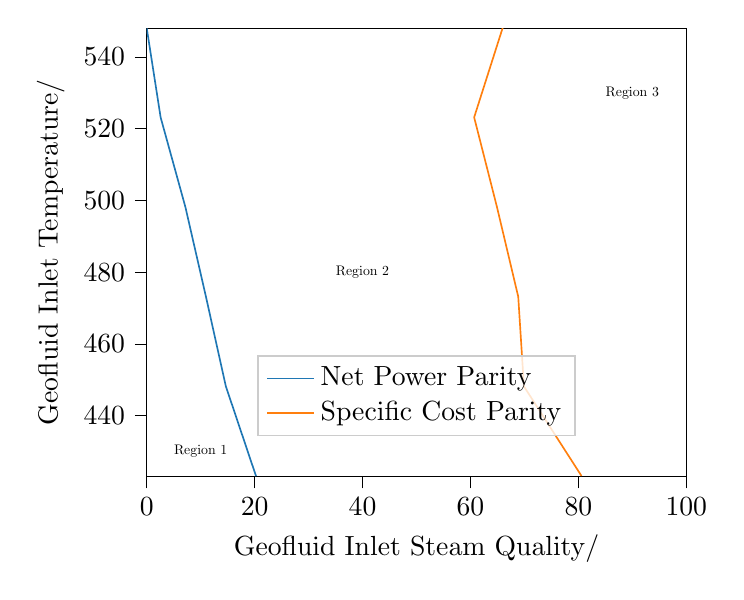
\begin{tikzpicture}

\definecolor{darkgray176}{RGB}{176,176,176}
\definecolor{darkorange25512714}{RGB}{255,127,14}
\definecolor{lightgray204}{RGB}{204,204,204}
\definecolor{steelblue31119180}{RGB}{31,119,180}

\begin{axis}[
legend cell align={left},
legend style={
  fill opacity=0.8,
  draw opacity=1,
  text opacity=1,
  at={(0.5,0.09)},
  anchor=south,
  draw=lightgray204
},
tick align=outside,
tick pos=left,
x grid style={darkgray176},
xlabel={Geofluid Inlet Steam Quality/\unit{\percent}},
xmin=0, xmax=100,
xtick style={color=black},
y grid style={darkgray176},
ylabel={Geofluid Inlet Temperature/\unit{\K}},
ymin=423, ymax=548,
ytick style={color=black}
]
\addplot [semithick, steelblue31119180]
table {%
20.2574810001872 423.15
14.6736248492937 448.15
10.9828903695487 473.15
7.17456971654515 498.15
2.5857550533881 523.15
0 548.15
};
\addlegendentry{Net Power Parity}
\addplot [semithick, darkorange25512714]
table {%
80.5840390695152 423.15
69.9083413304653 448.15
68.8529408109643 473.15
64.9111763437638 498.15
60.6841000655588 523.15
65.9803998207952 548.15
};
\addlegendentry{Specific Cost Parity}
\draw (axis cs:10,430) node[
  scale=0.5,
  text=black,
  rotate=0.0
]{Region 1};
\draw (axis cs:40,480) node[
  scale=0.5,
  text=black,
  rotate=0.0
]{Region 2};
\draw (axis cs:90,530) node[
  scale=0.5,
  text=black,
  rotate=0.0
]{Region 3};
\end{axis}

\end{tikzpicture}

        \caption[The geofluid inlet conditions for which the binary ORC and single flash \ac{DSC} geothermal power plants deliver equal net electrical power and have equal specific plant costs.]{The geofluid inlet conditions for which the binary ORC and single flash \ac{DSC} geothermal power plants deliver equal net electrical power and have equal specific plant costs. For the binary ORC, the specific plant cost is the minimum across all working fluids considered.}
        \label{fig:prosim_purewater_Breakeven_DSC_vs_ORC_SpecCost_techno}
    \end{figure}

    Alternatively, based on the net electrical power, it can be seen that the binary \ac{ORC} can compete up to geofluid inlet vapour qualities of \qtyrange{10}{30}{\percent}, Figure~\ref{fig:prosim_purewater_Wnet_DSC_vs_ORC_techno} and at similar specific plant costs to the single flash \ac{DSC}. 
    \begin{figure}[H]
        \centering
        % This file was created with tikzplotlib v0.10.1.
\begin{tikzpicture}

\definecolor{chocolate2369815}{RGB}{236,98,15}
\definecolor{darkgray165}{RGB}{165,165,165}
\definecolor{darkgray176}{RGB}{176,176,176}
\definecolor{darkslategray45}{RGB}{45,45,45}
\definecolor{dimgray108}{RGB}{108,108,108}
\definecolor{firebrick175572}{RGB}{175,57,2}
\definecolor{gainsboro216}{RGB}{216,216,216}
\definecolor{lightgray204}{RGB}{204,204,204}
\definecolor{lightsteelblue157201224}{RGB}{157,201,224}
\definecolor{midnightblue848107}{RGB}{8,48,107}
\definecolor{navajowhite253207161}{RGB}{253,207,161}
\definecolor{powderblue197218238}{RGB}{197,218,238}
\definecolor{saddlebrown127394}{RGB}{127,39,4}
\definecolor{sandybrown25315378}{RGB}{253,153,78}
\definecolor{sandybrown253173106}{RGB}{253,173,106}
\definecolor{silver188}{RGB}{188,188,188}
\definecolor{skyblue127184218}{RGB}{127,184,218}
\definecolor{steelblue59139194}{RGB}{59,139,194}
\definecolor{teal1287160}{RGB}{12,87,160}

\begin{groupplot}[group style={group size=1 by 2}]
\nextgroupplot[
legend cell align={left},
legend style={fill opacity=0.8, draw opacity=1, text opacity=1, draw=lightgray204},
tick align=outside,
tick pos=left,
x grid style={darkgray176},
xlabel={Inlet Steam Quality/\unit{\percent}},
xmin=-5, xmax=105,
xtick style={color=black},
y grid style={darkgray176},
ylabel={Net electric power/\unit{\mega\watt}},
ymin=0, ymax=30,
ytick style={color=black}
]
\addplot [semithick, skyblue127184218]
table {%
0 -1
1 -1
};
\addlegendentry{Binary ORC}
\addplot [semithick, chocolate2369815]
table {%
0 -1
1 -1
};
\addlegendentry{Single flash DSC}
\addplot [semithick, gainsboro216]
table {%
0 1
1 1
};
\addlegendentry{\(T_{geo}^{in}=\)\qty{423}{\K}}
\addplot [semithick, silver188]
table {%
0 1
1 1
};
\addlegendentry{\(T_{geo}^{in}=\)\qty{448}{\K}}
\addplot [semithick, darkgray165]
table {%
0 1
1 1
};
\addlegendentry{\(T_{geo}^{in}=\)\qty{473}{\K}}
\addplot [semithick, dimgray108]
table {%
0 1
1 1
};
\addlegendentry{\(T_{geo}^{in}=\)\qty{498}{\K}}
\addplot [semithick, darkslategray45]
table {%
0 1
1 1
};
\addlegendentry{\(T_{geo}^{in}=\)\qty{523}{\K}}
\addplot [semithick, black]
table {%
0 1
1 1
};
\addlegendentry{\(T_{geo}^{in}=\)\qty{548}{\K}}
\addplot [semithick, powderblue197218238, forget plot]
table {%
0 0.960849687129581
10 2.14458569253811
20 3.23035885785677
30 4.27566680248484
40 5.00700544345708
50 5.86983853781537
60 7.0594488651544
70 7.93193718867346
80 8.93664837449323
100 10.3793750090752
};
\addplot [semithick, lightsteelblue157201224, forget plot]
table {%
0 1.50952974466483
10 2.62305472157002
20 5.13252644589229
30 4.57207068080773
40 5.1310978081115
50 5.87176342204058
60 7.11533208609615
70 7.39108765599484
80 8.22080579508858
100 15.3542513774987
};
\addplot [semithick, skyblue127184218, forget plot]
table {%
0 2.09801582575957
10 3.59825615669869
20 3.89507826651621
30 4.66246522274257
40 5.48383732096798
50 6.32697641805644
60 7.05923199079413
70 8.07467669867112
80 8.93821959686381
100 10.7181908644327
};
\addplot [semithick, steelblue59139194, forget plot]
table {%
0 2.72625581513927
10 4.27047342573569
20 5.72840856540256
30 6.89239857439898
40 8.12016385080602
50 8.88948575778284
60 10.3053070490078
70 11.5409117007058
80 12.6644711957681
100 14.8640801493018
};
\addplot [semithick, teal1287160, forget plot]
table {%
0 3.40981980098837
10 4.70211364120694
20 6.01522355697679
30 7.03110269087159
40 8.1430117390292
50 9.0887040876772
60 10.2269550781848
70 11.1570874630651
80 12.1982183362838
100 14.4174746039932
};
\addplot [semithick, midnightblue848107, forget plot]
table {%
0 4.03006986002843
10 5.40480345953533
20 6.42088686926434
30 7.37991543828771
40 8.37226810980826
50 9.21659321716415
60 10.2901081894353
70 11.1013053206093
80 12.3122709020346
100 14.0852296591021
};
\addplot [semithick, navajowhite253207161, forget plot]
table {%
0 0.557114149477613
10 1.638809379093
20 3.21412473778287
30 4.88993046912543
40 6.40119018667188
50 8.01183196896339
60 9.44767830676006
70 10.8199603723257
80 12.2488536362307
100 15.2483801805043
};
\addplot [semithick, sandybrown253173106, forget plot]
table {%
0 1.08066458863151
10 2.2510134932247
20 3.92997004383771
30 5.74272006643475
40 7.49889052798885
50 9.71407527195079
60 11.2066841203576
70 13.5069457281367
80 14.7331560417993
100 18.7500172587311
};
\addplot [semithick, sandybrown25315378, forget plot]
table {%
0 1.64052050679576
10 2.87437434461262
20 4.43651027514178
30 6.54064816254777
40 8.79912360916101
50 10.7969730793877
60 12.751824036599
70 15.3704403856425
80 17.1222600178921
100 20.7412826958224
};
\addplot [semithick, chocolate2369815, forget plot]
table {%
0 2.30555058647817
10 3.65977973139912
20 4.83127169874635
30 7.24894705666434
40 9.50696724488665
50 11.9924728626009
60 13.6748087725596
70 16.757977411243
80 18.9233907014631
100 23.2626803222292
};
\addplot [semithick, firebrick175572, forget plot]
table {%
0 3.14394468871166
10 4.57715473188939
20 5.88207130807426
30 7.59483919695904
40 10.0956998814759
50 13.0154460785487
60 15.5655359107965
70 17.8582574715776
80 20.0412390531391
100 25.2823359007929
};
\addplot [semithick, saddlebrown127394, forget plot]
table {%
0 4.04694608432612
10 5.56385477936918
20 6.78431620199085
30 8.51801675553119
40 10.9574501504885
50 13.4872385647876
60 16.0443522656724
70 18.7578315602252
80 21.4234178239481
100 26.2259847001766
};
\addplot [semithick, red, mark=*, mark size=3, mark options={solid}, only marks]
table {%
20.2574810001872 3.25727355136542
25.0672234506447 4.84853098630374
15.7209666111048 3.76806709466906
27.155997056422 6.56135947321086
21.9106672040425 6.20932425141718
0 4.04694608432612
};
\addlegendentry{Break-even}

\nextgroupplot[
legend cell align={left},
legend style={fill opacity=0.8, draw opacity=1, text opacity=1, draw=lightgray204},
tick align=outside,
tick pos=left,
x grid style={darkgray176},
xlabel={Inlet Steam Quality/\unit{\percent}},
xmin=-5, xmax=105,
xtick style={color=black},
y grid style={darkgray176},
ylabel={Specific Cost/\unit{\USD\of{2023}\kilo\watt}},
ymin=0, ymax=6000,
ytick style={color=black}
]
\addplot [semithick, powderblue197218238, forget plot]
table {%
0 5019.56547982306
10 2522.57106687602
20 2240.69951062353
30 2053.98683462622
40 1941.96587910678
50 1842.47234948347
60 1780.06832167425
70 1726.41617758276
80 1686.31698562254
100 1602.83504349693
};
\addplot [semithick, lightsteelblue157201224, forget plot]
table {%
0 2744.8946588861
10 2272.38543986691
20 3348.05408810455
30 1882.88408329855
40 1771.02522520651
50 1688.72521989823
60 1631.21205136017
70 1574.09109359846
80 1533.21516140621
100 2205.44172551837
};
\addplot [semithick, skyblue127184218, forget plot]
table {%
0 2405.49149207129
10 3097.84203214475
20 1910.86221173232
30 1786.31917938869
40 1692.84297911923
50 1620.69761919165
60 1608.72937527545
70 1559.30680599622
80 1497.69192144539
100 1417.43111503078
};
\addplot [semithick, steelblue59139194, forget plot]
table {%
0 2198.3771443697
10 2622.27468624185
20 2308.61160681393
30 2113.50877997879
40 1983.50285339464
50 1884.01973590842
60 1785.66175509507
70 1723.64384618247
80 1668.84963609376
100 1569.36440336915
};
\addplot [semithick, teal1287160, forget plot]
table {%
0 2765.12486847892
10 2301.36862785584
20 2055.65553040038
30 1889.16536367077
40 1775.25384422885
50 1688.64847789024
60 1626.58498625757
70 1569.94847324597
80 1501.58429232089
100 1419.16357696616
};
\addplot [semithick, midnightblue848107, forget plot]
table {%
0 2364.49395107708
10 2082.70271598588
20 1902.65310939968
30 1778.30302161461
40 1681.76596511172
50 1605.11369334188
60 1540.95964264706
70 1487.43202350552
80 1443.68293367015
100 1365.31239325101
};
\addplot [semithick, navajowhite253207161, forget plot]
table {%
0 4888.7143335263
10 3404.0250225565
20 2765.54563623294
30 2409.1559187536
40 2183.27858115757
50 2009.69985620321
60 1878.59416928319
70 1781.0224664262
80 1687.7740515826
100 1554.39592832416
};
\addplot [semithick, sandybrown253173106, forget plot]
table {%
0 4151.52655916405
10 3093.66458210808
20 2505.74674359629
30 2179.5159627031
40 1957.18513763749
50 1799.12235928086
60 1671.81829312684
70 1573.71545917379
80 1494.37146800752
100 1352.99672129195
};
\addplot [semithick, sandybrown25315378, forget plot]
table {%
0 3655.98032140456
10 2848.07438984096
20 2334.75521170762
30 2013.49500986261
40 1811.64639061245
50 1658.35478306289
60 1536.22860528175
70 1435.11969747933
80 1358.52998816526
100 1238.4966377997
};
\addplot [semithick, chocolate2369815, forget plot]
table {%
0 3287.81162533514
10 2646.12175390539
20 2229.84454889565
30 1914.53283550025
40 1708.56313786346
50 1561.84904973759
60 1460.04569452233
70 1351.78587022443
80 1276.63372935777
100 1158.48133985561
};
\addplot [semithick, firebrick175572, forget plot]
table {%
0 2990.67224582709
10 2482.06128606799
20 2131.63812586402
30 1851.79844429968
40 1651.15991464286
50 1500.51750608008
60 1386.25897980577
70 1297.77276358557
80 1226.84937810228
100 1105.73508294575
};
\addplot [semithick, saddlebrown127394, forget plot]
table {%
0 2759.98967849107
10 2339.78553853144
20 2056.06477249343
30 1810.13960903689
40 1612.61074215184
50 1466.83729484511
60 1357.69912260723
70 1266.77667555141
80 1194.20844445113
100 1078.92746231424
};
\addplot [semithick, red, mark=*, mark size=3, mark options={solid}, only marks]
table {%
80.5840390695152 1683.87914983252
14.9367985901707 2803.42138647796
8.33516703959791 2982.5772322181
12.3239556472682 2549.38077776425
26.7033895623133 1944.05068581207
33.1523929813526 1747.8707476786
};
\addlegendentry{Break-even}
\end{groupplot}

\end{tikzpicture}

        \caption[The net electrical plant power and the corresponding specific plant cost of the single flash \ac{DSC} and the binary \ac{ORC}.]{The net electrical plant power (left) and the corresponding specific plant cost (right) of the single flash \ac{DSC} and the binary \ac{ORC}. For the binary \ac{ORC}, the net power is the maximum across all working fluids considered.}
        \label{fig:prosim_purewater_Wnet_DSC_vs_ORC_techno}
    \end{figure}

    From a geofluid inlet conditions perspective, four feasibility regions can be identified:
    \begin{description}
       \item[Region 1] Left of the blue line (representing parity in net power) and left of the yellow line (representing parity in specific plant cost), where the binary \ac{ORC} produces more net electrical power and at a lower specific plant cost compared to the single flash \ac{DSC}.
       \item[Region 2a] Right of the blue line and left of the yellow line, where the binary \ac{ORC} produces less net electrical power than the single flash \ac{DSC}, albeit at a lower specific cost.
      \item[Region 2b] Left of the blue line and right of the yellow line, where the binary \ac{ORC} produces more net electrical power than the single flash \ac{DSC}, but at a higher specific cost.
       \item[Region 3] Right of the yellow line, where the single flash \ac{DSC} produces more net electrical power and at a lower specific plant cost than the binary \ac{ORC}.
    \end{description}

    \begin{figure}[H]
        \centering
        % This file was created with tikzplotlib v0.10.1.
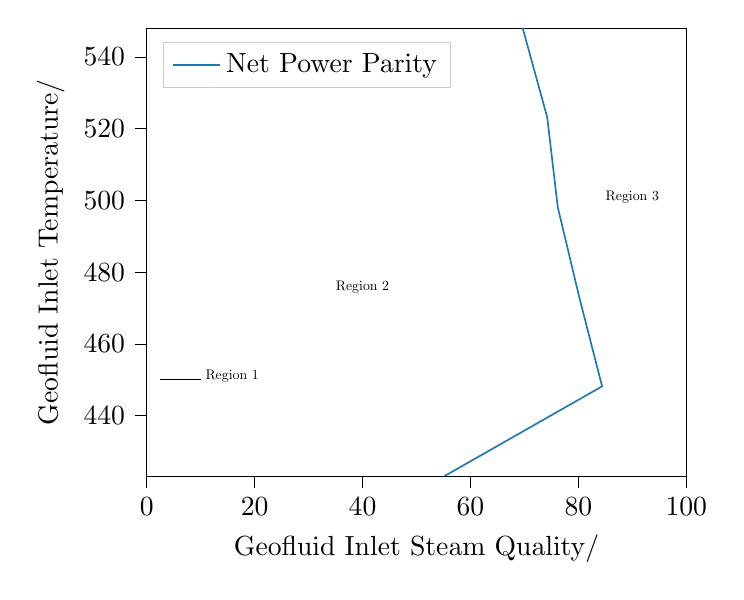
\begin{tikzpicture}

\definecolor{darkgray176}{RGB}{176,176,176}
\definecolor{lightgray204}{RGB}{204,204,204}
\definecolor{steelblue31119180}{RGB}{31,119,180}

\begin{axis}[
legend cell align={left},
legend style={
  fill opacity=0.8,
  draw opacity=1,
  text opacity=1,
  at={(0.03,0.97)},
  anchor=north west,
  draw=lightgray204
},
tick align=outside,
tick pos=left,
x grid style={darkgray176},
xlabel={Geofluid Inlet Steam Quality/\unit{\percent}},
xmin=0, xmax=100,
xtick style={color=black},
y grid style={darkgray176},
ylabel={Geofluid Inlet Temperature/\unit{\K}},
ymin=423, ymax=548,
ytick style={color=black}
]
\addplot [semithick, steelblue31119180]
table {%
55.2134270857992 423.15
84.3915070118743 448.15
80.1380984691528 473.15
76.1728044702929 498.15
74.2247944087056 523.15
69.6556133694898 548.15
};
\addlegendentry{Net Power Parity}
\draw (axis cs:90,500) node[
  scale=0.5,
  anchor=base,
  text=black,
  rotate=0.0
]{Region 3};
\draw (axis cs:40,475) node[
  scale=0.5,
  anchor=base,
  text=black,
  rotate=0.0
]{Region 2};
\draw[-,draw=black] (axis cs:10,450) -- (axis cs:2.5,450);
\draw (axis cs:10,450) node[
  scale=0.5,
  anchor=base west,
  text=black,
  rotate=0.0
]{Region 1};
\end{axis}

\end{tikzpicture}

        \caption[The geofluid inlet conditions for which the binary ORC and single flash DSC geothermal power plants deliver equal net electrical power and have equal specific plant costs.]{The geofluid inlet conditions for which the binary ORC and single flash DSC geothermal power plants deliver equal net electrical power and have equal specific plant costs. For the binary ORC, the net electrical power is the maximum across all working fluids considered.}
        \label{fig:prosim_purewater_Breakeven_DSC_vs_ORC_Wnet_techno}
    \end{figure}

    % \begin{figure}[H]
    %     \centering
    %     % This file was created with tikzplotlib v0.10.1.
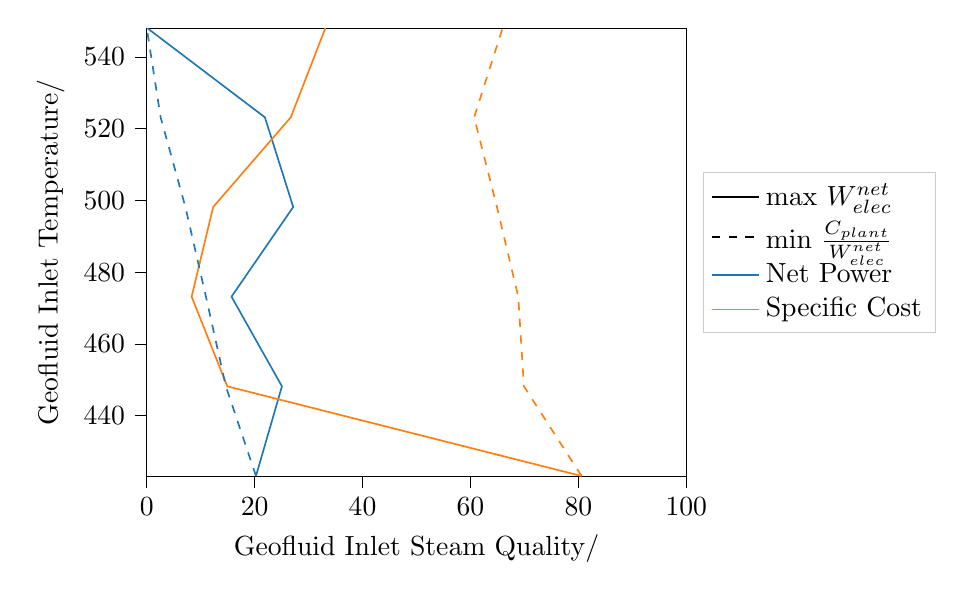
\begin{tikzpicture}

\definecolor{darkgray176}{RGB}{176,176,176}
\definecolor{darkorange25512714}{RGB}{255,127,14}
\definecolor{lightgray204}{RGB}{204,204,204}
\definecolor{steelblue31119180}{RGB}{31,119,180}

\begin{axis}[
legend cell align={left},
legend style={
  fill opacity=0.8,
  draw opacity=1,
  text opacity=1,
  at={(1.03,0.5)},
  anchor=west,
  draw=lightgray204
},
tick align=outside,
tick pos=left,
x grid style={darkgray176},
xlabel={Geofluid Inlet Steam Quality/\unit{\percent}},
xmin=0, xmax=100,
xtick style={color=black},
y grid style={darkgray176},
ylabel={Geofluid Inlet Temperature/\unit{\K}},
ymin=423, ymax=548,
ytick style={color=black}
]
\addplot [semithick, black]
table {%
0 -1
1 -1
};
\addlegendentry{max \(W_{elec}^{net}\)}
\addplot [semithick, black, dashed]
table {%
0 -1
1 -1
};
\addlegendentry{min \(\frac{C_{plant}}{W_{elec}^{net}}\)}
\addplot [semithick, steelblue31119180]
table {%
20.2574810001872 423.15
25.0672234506447 448.15
15.7209666111048 473.15
27.155997056422 498.15
21.9106672040425 523.15
0 548.15
};
\addlegendentry{Net Power}
\addplot [semithick, darkorange25512714]
table {%
80.5840390695152 423.15
14.9367985901707 448.15
8.33516703959791 473.15
12.3239556472682 498.15
26.7033895623133 523.15
33.1523929813526 548.15
};
\addlegendentry{Specific Cost}
\addplot [semithick, steelblue31119180, dashed, forget plot]
table {%
20.2574810001872 423.15
14.6736248492937 448.15
10.9828903695487 473.15
7.17456971654515 498.15
2.5857550533881 523.15
0 548.15
};
\addplot [semithick, darkorange25512714, dashed, forget plot]
table {%
80.5840390695152 423.15
69.9083413304653 448.15
68.8529408109643 473.15
64.9111763437638 498.15
60.6841000655588 523.15
65.9803998207952 548.15
};
\end{axis}

\end{tikzpicture}

    %     \caption{The geofluid inlet conditions for which the binary \ac{ORC} outperforms the single flash \ac{DSC}.}
    %     \label{fig:prosim_purewater_Breakeven_DSC_vs_ORC_techno}
    % \end{figure}            

\subsection{Conclusions}
    For the single flash \ac{DSC}, specific cost reductions of about \qtyrange{6}{10}{\percent}, at the expense of around \qtyrange{10}{20}{\percent} of net electrical power were observed. The cost reductions are almost entirely a result of a reduction in condenser size, by raising the minimum approach temperature difference and condensation temperature. For the binary \ac{ORC}, larger cost reductions of about \qtyrange{20}{30}{\percent} were observed, at the expense of up to \qty{65}{\percent} net electrical power. For all fluids the condenser costs are reduced by raising the minimum approach temperature difference and condensation temperature, for the heavier working fluids simultaneously reducing the number of turbine stages from a maximum of 5 to a minimum of 1. Nevertheless, n-Butane achieves the lowest specific net electrical power across a broad range of geofluid inlet conditions.
    
    From a specific cost perspective, techno-economically optimised binary ORCs can compete with single flash DSCs to geofluid inlet vapour qualities as high as \qty{80}{\percent}, but produce significantly less power. Here, the envelope for competitive specific power and net electrical power reduces from a geofluid inlet vapour quality of \qty{20}{\percent} at a geofluid inlet temperature \qty{423}{\K} to \qty{0}{\percent} at \qty{548}{\K}.

\clearpage
